\documentclass[a4paper,12pt]{article}

\usepackage[utf8]{inputenc}
\usepackage[top=3cm, bottom=3cm, left=3cm, right=3cm]{geometry}
\usepackage{indentfirst}
\usepackage{enumitem}
\usepackage{tikz}
\usepackage{pifont} % For checkmark and xmark with ding.

\newcommand{\ra}{$\rightarrow$ }
\newcommand{\lra}{$\leftrightarrow$ }
\newcommand{\s}{$\sim$}
\newcommand{\vd}{$\vdash$ }

\newcommand{\cmark}{\ding{51}}
\newcommand{\xmark}{\ding{55}}

\newcommand{\tb}{\textbar \ }

\begin{document}

    \begin{titlepage}
        \begin{center}
            \textsc{\large Exercise solutions for\\
            Logic\\
            by Paul Tomassi}\\[1.5cm]
            \textsc{D. G. O.}
        \end{center}
    \end{titlepage}

    \newpage

    \section*{Chapter One: How to Think Logically}

    \subsection*{EXERCISE 1.1}

    \begin{enumerate}[label=\arabic*,leftmargin=*]
        \item
            \nopagebreak
            \begin{enumerate}[label=\Alph*]
                \item Not an argument. There are no premises and there is no conclusion.
                \item Argument. First two sentences are premises, and the "so" in the third sentence indicates it is a conclusion.
                \item Argument. First two sentences are premises, and the "therefore" in the third sentence indicates it is a conclusion.
                \item Not an argument. There are no premises and there is no conclusion.
            \end{enumerate}

        \item
            \nopagebreak
            \begin{enumerate}[label=\Alph*]
                \item \textbf{Premises}\\
                    Professor Plum was in the drawing room and Miss Scarlet was in the conservatory. If Professor Plum was in the drawing room and the murder weapon was found in the drawing room then Professor Plum is in big trouble.\\
                    \textbf{Conclusion}\\
                    So, if the murder weapon was found in the drawing room then Professor Plum really is in big trouble\\
                    \textbf{Reasons}\\
                    The conclusion follows from the premises, and the "so" word in the last sentence indicates a conclusion.

                \item \textbf{Premises}\\
                    All human beings are mortal. After all, he is a human being.\\
                    \textbf{Conclusion}\\
                    So, it stands to reason that Socrates is mortal.\\
                    \textbf{Reasons}\\
                    The conclusion follows from the premises, and the "so" word in the second sentence indicates a conclusion.

                \item \textbf{Premises}\\
                    Very few elephants can fly. Very few elephants are pink. For fewer pink elephants than ordinary elephants can actually fly.\\
                    \textbf{Conclusion}\\
                    So, the pink flying elephant is truly a rare creature.\\
                    \textbf{Reasons}\\
                    The conclusion follows from the premises, and these sentences are in the form of an argument with the words "so" and "for".

                \item \textbf{Premises}\\
                     For the murderer used the knife and Professor Plum had the knife. And the murder was comitted in the hall and Professor Plum was certainly in the hall earlier.\\
                    \textbf{Conclusion}\\
                    Professor Plum was obviously the murderer in this instance.\\
                    \textbf{Reasons}\\
                    The conclusion follows from the premises not deductively, but inductively. These sentences are in the form of an argument with the word "for".

            \end{enumerate}

        \item
            \nopagebreak
            \begin{enumerate}[label=\Alph*]
                \item An argument is valid if it is impossible that it's premises be true and its conclusion false. It follows, that if it is not a valid argument, then it is possible, that it's premises be true, and its conclusion false. Also, it is a valid argument only if it is impossible that it's premises be true and its conclusion false. It follows, that if it is possible that it's premises be true and its conclusion false, then it is an invalid argument. All in all, an argument is invalid if and only if it is possible that it's premises be true and its conclusion false.

                \item Yes, a valid argument can have false conclusion if and only if it has a false premise. In that case, the premise is false, which means that it is impossible that it's premises are true, and it's conclusion false.

                \item No, a for a valid argument it is not possible (impossible) to have true premises and false conclusion.

                \item No. It is impossible that a true premise be true, and a true conclusion to be false, therefore, it is a valid argument.

                \item No. A sound argument is both valid and has true premises.

                \item Yes. A sound argument is valid and has true premises. It is valid, so it is not true, that it's premises are true and it's conclusion false. The premises are true, therefore this last sentence can only be true if the conclusion is true.

                \item An argument form is valid if and only if every substitution-instance of that form is valid.

                \item An argument form is invalid if and only if there is any substitution-instance of that form that is invalid.

            \end{enumerate}

        \item
            \nopagebreak
            \begin{enumerate}[label=\Alph*]
                \item Valid, not sound.
                \item Invalid. We do not know whether "better than" in this context is transitive.
                \item Invalid.
                \item Invalid.
            \end{enumerate}

        \item
            \nopagebreak
            \begin{enumerate}[label=(\roman*)]
                \item C If $p$ then $q$. $q$. Therefore, $p$.
                    D If $p$ then $q$. Not $p$. Therefore, not $q$.
                \item Yes, because both premises are true, but both conclusions are not true.
            \end{enumerate}

        \item If I clean my room, then it is not the case, that there is dirt on the floor. It is not the case, that I clean my room. Therefore, there is no dirt on the floor.

        \item By the definition given in this chapter, sentential variable is a variable, whose value is a well-formed sentence. Both 1 and 2 are one whole sentence which cannot be divided. The whole argument then is: $p$ therefore, $q$.
            \begin{enumerate}[label=(\roman*)]
                \item No, it is not a valid form. Counterexample is where $p$ is "snow is white", $q$ is "there are pink elephants". Here $p$ is true, and $q$ is not, then it is not not true, that $p$ is true and $q$ is false.
                \item Yes, intuitively (or modally) it is a valid argument, because it is not true, that the premise be true and the conclusion be false.
            \end{enumerate}

    \end{enumerate}

    \newpage

    \section*{Chapter Two:\\How to Prove that You Can Argue Logically \#1}

    \subsection*{EXERCISE 2.1}

    \begin{enumerate}[label=\arabic*,leftmargin=*]
        \item The main connective in each case are
            \nopagebreak
            \begin{enumerate}[label=(\roman*)]
                \begin{minipage}{0.5\linewidth}
                    \item conjunction,
                    \item negation,
                    \item conjunction,
                    \item conjunction,
                    \item disjunction,
                \end{minipage}
                \begin{minipage}{0.5\linewidth}
                    \item disjunction,
                    \item conditional,
                    \item conjunction,
                    \item biconditional,
                    \item biconditional.
                \end{minipage}
            \end{enumerate}

        \item For (ii) and (x) it's the whole formula. For (iii) it's \s P and \s Q.\\
            For (iv) it's \s (P \& Q) and \s Q.

        \item The key is
            P: Blind Lemon Jefferson is the only bluesman.\\
            Q: Dr Strangely Strange is a bluesman.\\
            R: Mr Oddly Normal is a bluesman.\\
            S: Blind Lemon Jefferson is a milkman.\\
            T: Blind Lemon Jefferson is a bluesman.\\
            U: Blind Lemon recorded it.\\
            V: It's a blues album.\\
            The sentences translated to PL are

            \begin{enumerate}[label=(\roman*)]
                \item \s P,
                \item \s Q \& \s R,
                \item S \ra \s T,
                \item \s (U \ra \s V),
                \item S v T,
                \item \s (S v T).
            \end{enumerate}

        \item The trees are the followings.
            \nopagebreak
            \begin{enumerate}[label=(\roman*)]
                \begin{minipage}{\textwidth}
                \item P \& Q \\
                    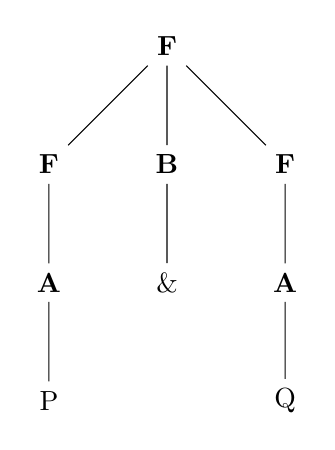
\begin{tikzpicture}
                        \tikzstyle{level 1}=[sibling distance=15mm]
                        \tikzstyle{level 2}=[sibling distance=15mm]
                        \node{\textbf{F}}
                            child {node {\textbf{F}}
                                child {node {\textbf{A}}
                                    child {node {P}
                                    }
                                }
                            }
                            child {node {\textbf{B}}
                                child {node {\&}
                                }
                            }
                            child {node {\textbf{F}}
                                child {node {\textbf{A}}
                                    child {node {Q}
                                    }
                                }
                            };
                    \end{tikzpicture}
                \end{minipage}
                \begin{minipage}{\textwidth}
                \item \s (P \& Q) \\
                    \begin{tikzpicture}
                        \tikzstyle{level 1}=[sibling distance=30mm]
                        \tikzstyle{level 2}=[sibling distance=15mm]
                        \node{\textbf{F}}
                            child {node {\textbf{U}}
                                child {node {\s }
                                }
                            }
                            child {node {\textbf{F}}
                                child {node {\textbf{F}}
                                    child {node {\textbf{A}}
                                        child {node {P}
                                        }
                                    }
                                }
                                child {node {\textbf{B}}
                                    child {node {\&}
                                    }
                                }
                                child {node {\textbf{F}}
                                    child {node {\textbf{A}}
                                        child {node {Q}
                                        }
                                    }
                                }
                            };
                    \end{tikzpicture}
                \end{minipage}
                \begin{minipage}{\textwidth}
                \item \s P \& \s Q \\
                    \begin{tikzpicture}
                        \tikzstyle{level 1}=[sibling distance=30mm]
                        \tikzstyle{level 2}=[sibling distance=15mm]
                        \node{\textbf{F}}
                            child {node {\textbf{F}}
                                child {node {\textbf{U}}
                                    child {node {\s }
                                    }
                                }
                                child {node {\textbf{F}}
                                    child {node {\textbf{A}}
                                        child {node {P}
                                        }
                                    }
                                }
                            }
                            child {node {\textbf{B}}
                                child {node {\&}
                                }
                            }
                            child {node {\textbf{F}}
                                child {node {\textbf{U}}
                                    child {node {\s }
                                    }
                                }
                                child {node {\textbf{F}}
                                    child {node {\textbf{A}}
                                        child {node {Q}
                                        }
                                    }
                                }
                            };
                    \end{tikzpicture}
                \end{minipage}
                \begin{minipage}{\textwidth}
                \item \s (P \& Q) \& (P \& \s Q) \\
                    \begin{tikzpicture}
                        \tikzstyle{level 1}=[sibling distance=30mm]
                        \tikzstyle{level 2}=[sibling distance=20mm]
                        \tikzstyle{level 3}=[sibling distance=10mm]
                        \node{\textbf{F}}
                            child {node {\textbf{F}}
                                child {node {\textbf{U}}
                                    child {node {\s }
                                    }
                                }
                                child {node {\textbf{F}}
                                    child {node {\textbf{F}}
                                        child {node {\textbf{A}}
                                            child {node {P}
                                            }
                                        }
                                    }
                                    child {node {\textbf{B}}
                                        child {node {\&}
                                        }
                                    }
                                    child {node {\textbf{F}}
                                        child {node {\textbf{A}}
                                            child {node {Q}
                                            }
                                        }
                                    }
                                }
                            }
                            child {node {\textbf{B}}
                                child {node {\&}
                                }
                            }
                            child {node {\textbf{F}}
                                child {node {\textbf{F}}
                                    child {node {\textbf{A}}
                                        child {node {P}
                                        }
                                    }
                                }
                                child {node {\textbf{B}}
                                    child {node {\&}
                                    }
                                }
                                child {node {\textbf{F}}
                                    child {node {\textbf{U}}
                                        child {node {\s }
                                        }
                                    }
                                    child {node {\textbf{F}}
                                        child {node {\textbf{A}}
                                            child {node {Q}
                                            }
                                        }
                                    }
                                }
                            };
                    \end{tikzpicture}
                \end{minipage}
                \begin{minipage}{\textwidth}
                \item P v Q\\
                    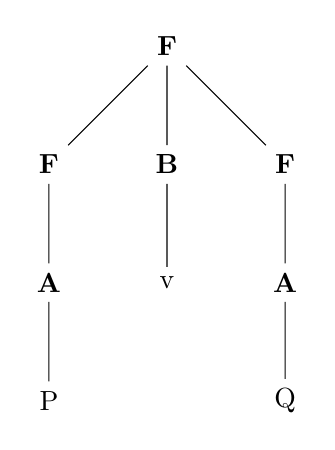
\begin{tikzpicture}
                        \tikzstyle{level 1}=[sibling distance=15mm]
                        \node{\textbf{F}}
                            child {node {\textbf{F}}
                                child {node {\textbf{A}}
                                    child {node {P}
                                    }
                                }
                            }
                            child {node {\textbf{B}}
                                child {node {v}
                                }
                            }
                            child {node {\textbf{F}}
                                child {node {\textbf{A}}
                                    child {node {Q}
                                    }
                                }
                            };
                    \end{tikzpicture}
                \end{minipage}
                \begin{minipage}{\textwidth}
                \item (P \& Q) v (Q \& R) \\
                    \begin{tikzpicture}
                        \tikzstyle{level 1}=[sibling distance=30mm]
                        \tikzstyle{level 2}=[sibling distance=20mm]
                        \tikzstyle{level 3}=[sibling distance=10mm]
                        \node{\textbf{F}}
                            child {node {\textbf{F}}
                                child {node {\textbf{F}}
                                    child {node {\textbf{A}}
                                        child {node {P}
                                        }
                                    }
                                }
                                child {node {\textbf{B}}
                                    child {node {\&}
                                    }
                                }
                                child {node {\textbf{F}}
                                    child {node {\textbf{A}}
                                        child {node {Q}
                                        }
                                    }
                                }
                            }
                            child {node {\textbf{B}}
                                child {node {v}
                                }
                            }
                            child {node {\textbf{F}}
                                child {node {\textbf{F}}
                                    child {node {\textbf{A}}
                                        child {node {Q}
                                        }
                                    }
                                }
                                child {node {\textbf{B}}
                                    child {node {\&}
                                    }
                                }
                                child {node {\textbf{F}}
                                    child {node {\textbf{A}}
                                        child {node {R}
                                        }
                                    }
                                }
                            };
                    \end{tikzpicture}
                \end{minipage}
                \begin{minipage}{\textwidth}
                \item P \ra Q\\
                    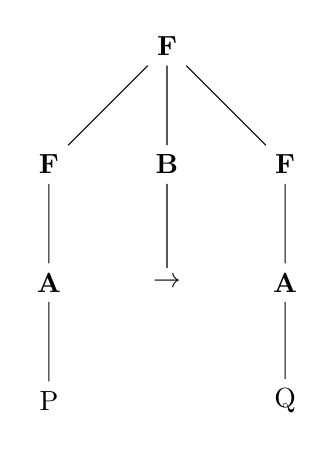
\begin{tikzpicture}
                        \tikzstyle{level 1}=[sibling distance=15mm]
                        \node{\textbf{F}}
                            child {node {\textbf{F}}
                                child {node {\textbf{A}}
                                    child {node {P}
                                    }
                                }
                            }
                            child {node {\textbf{B}}
                                child {node {\ra}
                                }
                            }
                            child {node {\textbf{F}}
                                child {node {\textbf{A}}
                                    child {node {Q}
                                    }
                                }
                            };
                    \end{tikzpicture}
                \end{minipage}
                \begin{minipage}{\textwidth}
                \item (P \ra Q) \& (Q \ra R) \\
                    \begin{tikzpicture}
                        \tikzstyle{level 1}=[sibling distance=30mm]
                        \tikzstyle{level 2}=[sibling distance=20mm]
                        \tikzstyle{level 3}=[sibling distance=10mm]
                        \node{\textbf{F}}
                            child {node {\textbf{F}}
                                child {node {\textbf{F}}
                                    child {node {\textbf{A}}
                                        child {node {P}
                                        }
                                    }
                                }
                                child {node {\textbf{B}}
                                    child {node {\ra}
                                    }
                                }
                                child {node {\textbf{F}}
                                    child {node {\textbf{A}}
                                        child {node {Q}
                                        }
                                    }
                                }
                            }
                            child {node {\textbf{B}}
                                child {node {\&}
                                }
                            }
                            child {node {\textbf{F}}
                                child {node {\textbf{F}}
                                    child {node {\textbf{A}}
                                        child {node {Q}
                                        }
                                    }
                                }
                                child {node {\textbf{B}}
                                    child {node {\ra}
                                    }
                                }
                                child {node {\textbf{F}}
                                    child {node {\textbf{A}}
                                        child {node {R}
                                        }
                                    }
                                }
                            };
                    \end{tikzpicture}
                \end{minipage}
                \begin{minipage}{\textwidth}
                \item (P \& Q) \lra (Q \& P) \\
                    \begin{tikzpicture}
                        \tikzstyle{level 1}=[sibling distance=30mm]
                        \tikzstyle{level 2}=[sibling distance=20mm]
                        \tikzstyle{level 3}=[sibling distance=10mm]
                        \node{\textbf{F}}
                            child {node {\textbf{F}}
                                child {node {\textbf{F}}
                                    child {node {\textbf{A}}
                                        child {node {P}
                                        }
                                    }
                                }
                                child {node {\textbf{B}}
                                    child {node {\&}
                                    }
                                }
                                child {node {\textbf{F}}
                                    child {node {\textbf{A}}
                                        child {node {Q}
                                        }
                                    }
                                }
                            }
                            child {node {\textbf{B}}
                                child {node {\lra}
                                }
                            }
                            child {node {\textbf{F}}
                                child {node {\textbf{F}}
                                    child {node {\textbf{A}}
                                        child {node {Q}
                                        }
                                    }
                                }
                                child {node {\textbf{B}}
                                    child {node {\&}
                                    }
                                }
                                child {node {\textbf{F}}
                                    child {node {\textbf{A}}
                                        child {node {P}
                                        }
                                    }
                                }
                            };
                    \end{tikzpicture}
                \end{minipage}
                \begin{minipage}{\textwidth}
                \item \s ((P \& Q) \lra (Q \& P)) \\
                    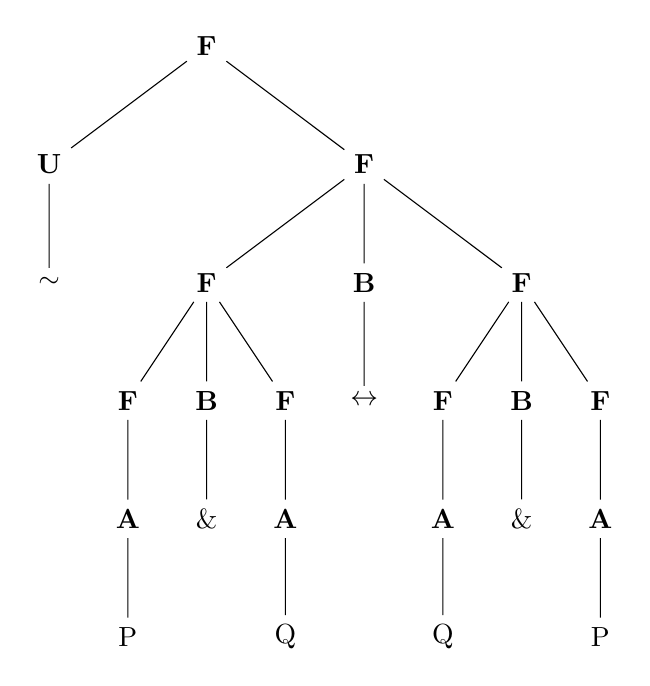
\begin{tikzpicture}
                        \tikzstyle{level 1}=[sibling distance=40mm]
                        \tikzstyle{level 2}=[sibling distance=20mm]
                        \tikzstyle{level 3}=[sibling distance=10mm]
                        \node{\textbf{F}}
                            child {node {\textbf{U}}
                                child {node {\s }
                                }
                            }
                            child {node {\textbf{F}}
                                child {node {\textbf{F}}
                                    child {node {\textbf{F}}
                                        child {node {\textbf{A}}
                                            child {node {P}
                                            }
                                        }
                                    }
                                    child {node {\textbf{B}}
                                        child {node {\&}
                                        }
                                    }
                                    child {node {\textbf{F}}
                                        child {node {\textbf{A}}
                                            child {node {Q}
                                            }
                                        }
                                    }
                                }
                                child {node {\textbf{B}}
                                    child {node {\lra}
                                    }
                                }
                                child {node {\textbf{F}}
                                    child {node {\textbf{F}}
                                        child {node {\textbf{A}}
                                            child {node {Q}
                                            }
                                        }
                                    }
                                    child {node {\textbf{B}}
                                        child {node {\&}
                                        }
                                    }
                                    child {node {\textbf{F}}
                                        child {node {\textbf{A}}
                                            child {node {P}
                                            }
                                        }
                                    }
                                }
                            };
                    \end{tikzpicture}
                \end{minipage}
            \end{enumerate}

    \end{enumerate}

    \subsection*{EXERCISE 2.2}

    \begin{enumerate}[label=\arabic*,leftmargin=*]

        \item P v Q, \s R \ra Q, \s R : \s P
            \nopagebreak
            \begin{enumerate}[label=(\roman*)]
                \item P: Big Bill Broonzy is a Delta bluesman.
                \item Q: Big Bill Broonzy is a Chicago bluesman.
                \item R: Big Bill Broonzy was born in Mississippi.
            \end{enumerate}
            This is an invalid sequent.

        \item \s (P \& Q), P : Q
            \nopagebreak
            \begin{enumerate}[label=(\roman*)]
                \item P: Etta James was an angel.
                \item Q: Robert Johnson sold his soul to the devil.
            \end{enumerate}
            This is a valid sequent.

        \item \s P \ra \s Q, \s (P \& \s R), R : Q
            \nopagebreak
            \begin{enumerate}[label=(\roman*)]
                \item P: There's light on in the Venue.
                \item Q: The band are on stage already.
                \item R: It's going to be a great night.
            \end{enumerate}
            This is an invalid sequent.

        \item P v Q, P \ra \s R, Q \ra \s R : \s R
            \nopagebreak
            \begin{enumerate}[label=(\roman*)]
                \item P: There's a punk rock band playing at the Venue tonight.
                \item Q: The music is strictly classical.
                \item R: There will be no blues at the Venue tonight.
            \end{enumerate}
            This is a valid sequent.

        \item (P \& Q) \ra \s R : R \ra (P \ra Q)
            \nopagebreak
            \begin{enumerate}[label=(\roman*)]
                \item P: There's a band on stage.
                \item Q: The music is groovy.
                \item R: It is the Nasal Flute Orchestra.
            \end{enumerate}
            This is an invalid sequent.

    \end{enumerate}

    \subsection*{EXERCISE 2.3}

    \begin{enumerate}[label=\arabic*,leftmargin=*]

        \item Dependencies, line number, formula, rule which was used in the line.

        \item The proofs are the followings.
            \nopagebreak
            \begin{enumerate}[label=\arabic*.]

                \begin{minipage}{\textwidth}
                \item P, Q : P \& Q
                    \vspace{1em}\\
                    \begin{tabular}{l l l l}
                        \{1\} & 1. & P & Premise \\
                        \{2\} & 2. & Q & Premise \\
                        \{1, 2\} & 3. & P \& Q & 1, 2 \&I \\
                    \end{tabular}
                    \vspace{1em}
                \end{minipage}
                \begin{minipage}{\textwidth}
                \item P, Q, R : (P \& Q) \& R
                    \vspace{1em}\\
                    \begin{tabular}{l l l l}
                        \{1\} & 1. & P & Premise \\
                        \{2\} & 2. & Q & Premise \\
                        \{3\} & 3. & R & Premise \\
                        \{1, 2\} & 4. & P \& Q & 1, 2 \&I \\
                        \{1, 2, 3\} & 5. & (P \& Q) \& R & 3, 4 \&I \\
                    \end{tabular}
                    \vspace{1em}
                \end{minipage}
                \begin{minipage}{\textwidth}
                \item P, Q, R, S : (P \& Q) \& (R \& S)
                    \vspace{1em}\\
                    \begin{tabular}{l l l l}
                        \{1\} & 1. & P & Premise \\
                        \{2\} & 2. & Q & Premise \\
                        \{3\} & 3. & R & Premise \\
                        \{4\} & 4. & S & Premise \\
                        \{1, 2\} & 5. & P \& Q & 1, 2 \&I \\
                        \{3, 4\} & 6. & R \& S & 3, 4 \&I \\
                        \{1, 2, 3, 4\} & 7. & (P \& Q) \& (R \& S) & 5, 6 \&I \\
                    \end{tabular}
                    \vspace{1em}
                \end{minipage}
                \begin{minipage}{\textwidth}
                \item P \& Q : P
                    \vspace{1em}\\
                    \begin{tabular}{l l l l}
                        \{1\} & 1. & (P \& Q) & Premise \\
                        \{1\} & 2. & P & 1 \&E \\
                    \end{tabular}
                    \vspace{1em}
                \end{minipage}
                \begin{minipage}{\textwidth}
                \item P \& Q : Q
                    \vspace{1em}\\
                    \begin{tabular}{l l l l}
                        \{1\} & 1. & (P \& Q) & Premise \\
                        \{1\} & 2. & Q & 1 \&E \\
                    \end{tabular}
                    \vspace{1em}
                \end{minipage}
                \begin{minipage}{\textwidth}
                \item (P \& Q) \& R : P
                    \vspace{1em}\\
                    \begin{tabular}{l l l l}
                        \{1\} & 1. & (P \& Q) \& R & Premise \\
                        \{1\} & 2. & P \& Q & 1 \&E \\
                        \{1\} & 3. & P & 2 \&E \\
                    \end{tabular}
                    \vspace{1em}
                \end{minipage}
                \begin{minipage}{\textwidth}
                \item (P \& Q) \& (R \& S) : P
                    \vspace{1em}\\
                    \begin{tabular}{l l l l}
                        \{1\} & 1. & (P \& Q) \& (R \& S) & Premise \\
                        \{1\} & 2. & P \& Q & 1 \&E \\
                        \{1\} & 3. & P & 2 \&E \\
                    \end{tabular}
                    \vspace{1em}
                \end{minipage}
                \begin{minipage}{\textwidth}
                \item (Q \& R), P : (P \& Q) \& R
                    \vspace{1em}\\
                    \begin{tabular}{l l l l}
                        \{1\} & 1. & Q \& R & Premise \\
                        \{2\} & 2. & P & Premise \\
                        \{1\} & 3. & Q & 1 \&E \\
                        \{1\} & 4. & R & 1 \&E \\
                        \{1, 2\} & 5. & P \& Q & 2, 3 \&I \\
                        \{1, 2\} & 6. & (P \& Q) \& R & 4, 5 \&I \\
                    \end{tabular}
                \end{minipage}

            \end{enumerate}

    \end{enumerate}

    \subsection*{EXERCISE 2.4}

    \begin{enumerate}[label=\arabic*,leftmargin=*]

        \item The proofs are the followings.
            \nopagebreak
            \begin{enumerate}[label=\arabic*.]

                \begin{minipage}{\textwidth}
                \item P \ra Q, P : Q
                    \vspace{1em}\\
                    \begin{tabular}{l l l l}
                        \{1\} & 1. & P \ra Q & Premise \\
                        \{2\} & 2. & P & Premise \\
                        \{1, 2\} & 3. & Q & 1, 2 MP \\
                    \end{tabular}
                    \vspace{1em}
                \end{minipage}
                \begin{minipage}{\textwidth}
                \item P \ra (P \ra Q), P : Q
                    \vspace{1em}\\
                    \begin{tabular}{l l l l}
                        \{1\} & 1. & P \ra (P \ra Q) & Premise \\
                        \{2\} & 2. & P & Premise \\
                        \{1, 2\} & 3. & P \ra Q & 1, 2 MP \\
                        \{1, 2\} & 4. & Q & 2, 3 MP \\
                    \end{tabular}
                    \vspace{1em}
                \end{minipage}
                \begin{minipage}{\textwidth}
                \item P \ra (P \& Q), P : Q
                    \vspace{1em}\\
                    \begin{tabular}{l l l l}
                        \{1\} & 1. & P \ra (P \& Q) & Premise \\
                        \{2\} & 2. & P & Premise \\
                        \{1, 2\} & 3. & P \& Q & 1, 2 MP \\
                        \{1, 2\} & 4. & Q & 3 \&E \\
                    \end{tabular}
                    \vspace{1em}
                \end{minipage}
                \begin{minipage}{\textwidth}
                \item P \ra (Q \ra R), P \ra Q, P : R
                    \vspace{1em}\\
                    \begin{tabular}{l l l l}
                        \{1\} & 1. & P \ra (Q \ra R) & Premise \\
                        \{2\} & 2. & P \ra Q & Premise \\
                        \{3\} & 3. & P & Premise \\
                        \{1, 3\} & 4. & Q \ra R & 1, 3 MP \\
                        \{2, 3\} & 5. & Q & 2, 3 MP \\
                        \{1, 2, 3\} & 6. & R & 4, 5 MP \\
                    \end{tabular}
                \end{minipage}

            \end{enumerate}

        \item The proofs are the followings.
            \nopagebreak
            \begin{enumerate}[label=(\roman*)]
                \begin{minipage}{\textwidth}
                \item P \ra (Q \& R), P \& Q : P \& R
                    \vspace{1em}\\
                    \begin{tabular}{l l l l}
                        \{1\} & 1. & P \ra (Q \& R) & Premise \\
                        \{2\} & 2. & P \& Q & Premise \\
                        \{2\} & 3. & P & 2 \&E \\
                        \{1, 2\} & 4. & Q \& R & 1, 3 MP \\
                        \{1, 2\} & 5. & R & 4 \&E \\
                        \{1, 2\} & 6. & P \& R & 3, 5 \&I \\
                    \end{tabular}
                    \vspace{1em}
                \end{minipage}
                \begin{minipage}{\textwidth}
                \item (P \ra Q) \ra (R \ra S), P \ra Q, P \& R : S
                    \vspace{1em}\\
                    \begin{tabular}{l l l l}
                        \{1\} & 1. & (P \ra Q) \ra (R \ra S) & Premise\\
                        \{2\} & 2. & P \ra Q & Premise\\
                        \{3\} & 3. & P \& R & Premise\\
                        \{1, 2\} & 4. & R \ra S & 1, 2 MP\\
                        \{3\} & 5. & R & 3 \&E\\
                        \{1, 2, 3\} & 6. & S & 4, 5 MP\\
                    \end{tabular}
                    \vspace{1em}
                \end{minipage}
                \begin{minipage}{\textwidth}
                \item P, P \ra Q : P \& Q
                    \vspace{1em}\\
                    \begin{tabular}{l l l l}
                        \{1\} & 1. & P & Premise\\
                        \{2\} & 2. & P \ra Q & Premise\\
                        \{1, 2\} & 3. & Q & 1, 2 MP\\
                        \{1, 2\} & 4. & P \& Q & 1, 3 \&I\\
                    \end{tabular}
                    \vspace{1em}
                \end{minipage}
                \begin{minipage}{\textwidth}
                \item P, P \ra Q, P \ra (Q \ra R) : P \& R
                    \vspace{1em}\\
                    \begin{tabular}{l l l l}
                        \{1\} & 1. & P & Premise\\
                        \{2\} & 2. & P \ra Q & Premise\\
                        \{3\} & 3. & P \ra (Q \ra R) & Premise\\
                        \{1, 2\} & 4. & Q & 1, 2 MP\\
                        \{1, 3\} & 5. & Q \ra R & 1, 3 MP\\
                        \{1, 2, 3\} & 6. & R & 4, 5 MP\\
                        \{1, 2, 3\} & 7. & P \& R & 1, 6 \&I\\
                    \end{tabular}
                    \vspace{1em}
                \end{minipage}
                \begin{minipage}{\textwidth}
                \item P, P \ra Q, P \ra (Q \ra R), R \ra S : (P \& Q) \& (R \& S)
                    \vspace{1em}\\
                    \begin{tabular}{l l l l}
                        \{1\} & 1. & P & Premise\\
                        \{2\} & 2. & P \ra Q & Premise\\
                        \{3\} & 3. & P \ra (Q \ra R) & Premise\\
                        \{4\} & 4. & R \ra S & Premise\\
                        \{1, 2\} & 5. & Q & 1, 2 MP\\
                        \{1, 3\} & 6. & Q \ra R & 1, 3 MP\\
                        \{1, 2, 3\} & 7. & R & 5, 6 MP\\
                        \{1, 2, 3\} & 8. & S & 4, 7 MP\\
                        \{1, 2\} & 9. & P \& Q & 1, 5 \&I\\
                        \{1, 2, 3\} & 10. & R \& S & 7, 8 \&I\\
                        \{1, 2, 3\} & 11. & (P \& Q) \& (R \& S) & 9, 10 \&I\\
                    \end{tabular}
                \end{minipage}

            \end{enumerate}

    \end{enumerate}

    \subsection*{EXERCISE 2.5}

    \begin{enumerate}[label=\arabic*,leftmargin=*]

        \item The proofs are the followings.
            \nopagebreak
            \begin{enumerate}[label=\arabic*.]

                \begin{minipage}{\textwidth}
                \item P \ra (Q \& R) : P \ra Q
                    \vspace{1em}\\
                    \begin{tabular}{l l l l}
                        \{1\} & 1. & P \ra (Q \& R) & Premise\\
                        \{2\} & 2. & P & Assumption for CP\\
                        \{1, 2\} & 3. & Q \& R & 1, 2 MP\\
                        \{1, 2\} & 4. & Q & 3 \&E\\
                        \{1\} & 5. & P \ra Q & 2, 4 CP\\
                    \end{tabular}
                    \vspace{1em}
                \end{minipage}
                \begin{minipage}{\textwidth}
                \item (P \& Q) \ra R, P : Q \ra R
                    \vspace{1em}\\
                    \begin{tabular}{l l l l}
                        \{1\} & 1. & (P \& Q) \ra R & Premise\\
                        \{2\} & 2. & P & Premise\\
                        \{3\} & 3. & Q & Assumption for CP\\
                        \{2, 3\} & 4. & P \& Q & 2, 3 \&I\\
                        \{1, 2, 3\} & 5. & R & 1, 4 MP\\
                        \{1, 2\} & 6. & Q \ra R & 3, 5 CP\\
                    \end{tabular}
                    \vspace{1em}
                \end{minipage}
                \begin{minipage}{\textwidth}
                \item (P \& Q), (P \& R) \ra S : R \ra S
                    \vspace{1em}\\
                    \begin{tabular}{l l l l}
                        \{1\} & 1. & P \& Q & Premise\\
                        \{2\} & 2. & (P \& R) \ra S & Premise\\
                        \{3\} & 3. & R & Assumtion for CP\\
                        \{1\} & 4. & P & 1 \&E\\
                        \{1, 3\} & 5. & P \& R & 3, 4 \&I\\
                        \{1, 2, 3\} & 6. & S & 2, 5 MP\\
                        \{1, 2\} & 7. & R \ra S & 3, 6 CP\\
                    \end{tabular}
                    \vspace{1em}\\
                \end{minipage}
                \begin{minipage}{\textwidth}
                \item (P \& Q) \ra R : P \ra (Q \ra R)
                    \vspace{1em}\\
                    \begin{tabular}{l l l l}
                        \{1\} & 1. & (P \& Q) \ra R & Premise\\
                        \{2\} & 2. & P & Assumption for CP\\
                        \{3\} & 3. & Q & Assumption for CP\\
                        \{2, 3\} & 4. & P \& Q & 2, 3 \&I\\
                        \{1, 2, 3\} & 5. & R & 1, 4 MP\\
                        \{1, 2\} & 6. & Q \ra R & 3, 5 CP\\
                        \{1\} & 7. & P \ra (Q \ra R) & 2, 6 CP\\
                    \end{tabular}
                    \vspace{1em}\\
                \end{minipage}
                \begin{minipage}{\textwidth}
                \item P \ra Q : (P \& R) \ra (R \& Q)
                    \vspace{1em}\\
                    \begin{tabular}{l l l l}
                        \{1\} & 1. & P \ra Q & Premise\\
                        \{2\} & 2. & P \& R & Assumption for CP\\
                        \{2\} & 3. & P & 2 \&E\\
                        \{1, 2\} & 4. & Q & 1, 3 MP\\
                        \{2\} & 5. & R & 2 \&E\\
                        \{1, 2\} & 6. & R \& Q & 4, 5 \&I\\
                        \{1\} & 7. & (P \& R) \ra (R \& Q) & 2, 6 CP\\
                    \end{tabular}
                    \vspace{1em}\\
                \end{minipage}
                \begin{minipage}{\textwidth}
                \item P \ra Q : (Q \ra R) \ra (P \ra R)
                    \vspace{1em}\\
                    \begin{tabular}{l l l l}
                        \{1\} & 1. & P \ra Q & Premise\\
                        \{2\} & 2. & Q \ra R & Assumption for CP\\
                        \{3\} & 3. & P & Assumption for CP\\
                        \{1, 3\} & 4. & Q & 1, 3 MP\\
                        \{1, 2, 3\} & 5. & R & 2, 4 MP\\
                        \{1, 2\} & 6. & P \ra R & 3, 5 CP\\
                        \{1\} & 7. & (Q \ra R) \ra (P \ra R) & 2, 6 CP\\
                    \end{tabular}
                    \vspace{1em}\\
                \end{minipage}
                \begin{minipage}{\textwidth}
                \item R \ra P, Q \ra S : (P \ra Q) \ra (R \ra S)
                    \vspace{1em}\\
                    \begin{tabular}{l l l l}
                        \{1\} & 1. & R \ra P & Premise\\
                        \{2\} & 2. & Q \ra S & Premise\\
                        \{3\} & 3. & P \ra Q & Assumption for CP\\
                        \{4\} & 4. & R & Assumption for CP\\
                        \{1, 4\} & 5. & P & 1, 4 MP\\
                        \{1, 3, 4\} & 6. & Q & 3, 5 MP\\
                        \{1, 2, 3, 4\} & 7. & S & 2, 6 MP\\
                        \{1, 2, 3\} & 8. & R \ra S & 4, 7 CP\\
                        \{1, 2\} & 9. & (P \ra Q) \ra (R \ra S) & 3, 8 CP\\
                    \end{tabular}
                    \vspace{1em}\\
                \end{minipage}
                \begin{minipage}{\textwidth}
                \item P \ra Q : (P \ra R) \ra (P \ra (Q \& R))
                    \vspace{1em}\\
                    \begin{tabular}{l l l l}
                        \{1\} & 1. & P \ra Q & Premise\\
                        \{2\} & 2. & P \ra R & Assumption for CP\\
                        \{3\} & 3. & P & Assumption for CP\\
                        \{1, 3\} & 4. & Q & 1, 3 MP\\
                        \{1, 2\} & 5. & R & 2, 3 MP\\
                        \{1, 2, 3\} & 6. & Q \& R & 4, 5 \&I\\
                        \{1, 2\} & 7. & P \ra (Q \& R) & 3, 6 CP\\
                        \{1\} & 8. & (P \ra R) \ra (P \ra (Q \& R)) & 2, 7 CP\\
                    \end{tabular}
                    \vspace{1em}\\
                \end{minipage}
                \begin{minipage}{\textwidth}
                \item P \ra (Q \ra R) : (S \ra Q) \ra (P \ra (S \ra R))
                    \vspace{1em}\\
                    \begin{tabular}{l l l l}
                        \{1\} & 1. & P \ra (Q \ra R) & Premise\\
                        \{2\} & 2. & S \ra Q & Assumption for CP\\
                        \{3\} & 3. & P & Assumption for CP\\
                        \{4\} & 4. & S & Assumption for CP\\
                        \{2, 4\} & 5. & Q & 2, 4 MP\\
                        \{1, 3\} & 6. & Q \ra R & 1, 3 MP\\
                        \{1, 2, 3, 4\} & 7. & R & 5, 6 MP\\
                        \{1, 2, 3\} & 8. & S \ra R & 4, 7 CP\\
                        \{1, 2\} & 9. & P \ra (S \ra R) & 3, 8 CP\\
                        \{1\} & 10. & (S \ra Q) \ra (P \ra (S \ra R)) & 2, 9 CP\\
                    \end{tabular}
                    \vspace{1em}\\
                \end{minipage}
                \begin{minipage}{\textwidth}
                \item P \ra Q : ((R \& Q) \ra S) \ra ((R \& P) \ra S)
                    \vspace{1em}\\
                    \begin{tabular}{l l l l}
                        \{1\} & 1. & P \ra Q & Premise\\
                        \{2\} & 2. & (R \& Q) \ra S & Assumption for CP\\
                        \{3\} & 3. & R \& P & Assumption for CP\\
                        \{3\} & 4. & P & 3 \&E\\
                        \{3\} & 5. & R & 3 \&E\\
                        \{1, 3\} & 6. & Q & 1, 4 MP\\
                        \{1, 3\} & 7. & R \& Q & 5, 6 \&I\\
                        \{1, 2, 3\} & 8. & S & 2, 7 MP\\
                        \{1, 2\} & 9. & (R \& P) \ra S & 3, 8 CP\\
                        \{1\} & 10. & ((R \& Q) \ra S) \ra ((R \& P) \ra S) & 2, 9 CP\\
                    \end{tabular}
                \end{minipage}

            \end{enumerate}

    \end{enumerate}

    \subsection*{EXERCISE 2.6}

    \begin{enumerate}[label=\arabic*,leftmargin=*]

        \item The proofs are the followings.
            \nopagebreak
            \begin{enumerate}[label=\arabic*.]

                \begin{minipage}{\textwidth}
                \item : ((P \ra P) \ra Q) \ra Q
                    \vspace{1em}\\
                    \begin{tabular}{l l l l}
                        \{1\} & 1. & P & Assumption for CP\\
                        -- & 2. & P \ra P & 1, 1 CP\\
                        \{3\} & 3. & (P \ra P) \ra Q & Assumption for CP\\
                        \{3\} & 4. & Q & 2, 3 MP\\
                        -- & 5. & ((P \ra P) \ra Q) \ra Q & 3, 4 CP\\
                    \end{tabular}
                    \vspace{1em}
                \end{minipage}
                \begin{minipage}{\textwidth}
                \item : (P \ra Q) \ra ((Q \ra R) \ra (P \ra R))
                    \vspace{1em}\\
                    \begin{tabular}{l l l l}
                        \{1\} & 1. & P \ra Q & Assumption for CP\\
                        \{2\} & 2. & Q \ra R & Assumption for CP\\
                        \{3\} & 3. & P & Assumption for CP\\
                        \{1, 3\} & 4. & Q & 1, 3 MP\\
                        \{1, 2, 3\} & 5. & R & 2, 4 MP\\
                        \{1, 2\} & 6. & P \ra R & 3, 5 CP\\
                        \{1\} & 7. & (Q \ra R) \ra (P \ra R) & 2, 6 CP\\
                        -- & 8. & (P \ra Q) \ra ((Q \ra R) \ra (P \ra R)) & 1, 7 CP\\
                    \end{tabular}
                    \vspace{1em}
                \end{minipage}
                \begin{minipage}{\textwidth}
                \item : (Q \ra R) \ra ((P \ra Q) \ra (P \ra R))
                    \vspace{1em}\\
                    \begin{tabular}{l l l l}
                        \{1\} & 1. & Q \ra R & Assumption for CP\\
                        \{2\} & 2. & P \ra Q & Assumption for CP\\
                        \{3\} & 3. & P & Assumption for CP\\
                        \{2, 3\} & 4. & Q & 2, 3 MP\\
                        \{1, 2, 3\} & 5. & R & 1, 4 MP\\
                        \{1, 2\} & 6. & P \ra R & 3, 5 CP\\
                        \{1\} & 7. & (P \ra Q) \ra (P \ra R) & 2, 6 CP\\
                        -- & 8. & (Q \ra R) \ra ((P \ra Q) \ra (P \ra R)) & 1, 7 CP\\
                    \end{tabular}
                    \vspace{1em}
                \end{minipage}
                \begin{minipage}{\textwidth}
                \item : P \ra (Q \ra (P \& Q))
                    \vspace{1em}\\
                    \begin{tabular}{l l l l}
                        \{1\} & 1. & P & Assumption for CP\\
                        \{2\} & 2. & Q & Assumption for CP\\
                        \{1, 2\} & 3. & P \& Q & 1, 2 \&I\\
                        \{1\} & 4. & Q \ra (P \& Q) & 2, 3 CP\\
                        -- & 5. & P \ra (Q \ra (P \& Q)) & 1, 4 CP\\
                    \end{tabular}
                \end{minipage}

            \end{enumerate}

    \end{enumerate}

    \subsection*{EXERCISE 2.7}

    \begin{enumerate}[label=\arabic*,leftmargin=*]

        \item The proofs are the followings.
            \nopagebreak
            \begin{enumerate}[label=\arabic*.]

                \begin{minipage}{\textwidth}
                \item P, P \lra Q : Q
                    \vspace{1em}\\
                    \begin{tabular}{l l l l}
                        \{1\} & 1. & P & Premise\\
                        \{2\} & 2. & P \lra Q & Premise\\
                        \{2\} & 3. & (P \ra Q) \& (Q \ra P) & \lra E\\
                        \{2\} & 4. & P \ra Q & 3 \&E\\
                        \{1, 2\} & 5. & Q & 1, 4 MP\\
                    \end{tabular}
                    \vspace{1em}
                \end{minipage}
                \begin{minipage}{\textwidth}
                \item P \& (P \lra Q) : P \& Q
                    \vspace{1em}\\
                    \begin{tabular}{l l l l}
                        \{1\} & 1. & P \& (P \lra Q) & Premise\\
                        \{1\} & 2. & P & 1 \&E\\
                        \{1\} & 3. & P \lra Q & 1 \&E\\
                        \{1\} & 4. & (P \ra Q) \& (Q \ra P) & 3 \lra E\\
                        \{1\} & 5. & P \ra Q & 4 \&E\\
                        \{1\} & 6. & Q & 2, 5 MP\\
                        \{1\} & 7. & P \& Q & 2, 6 \&I\\
                    \end{tabular}
                    \vspace{1em}
                \end{minipage}
                \begin{minipage}{\textwidth}
                \item (P \& Q) \lra P : P \ra Q
                    \vspace{1em}\\
                    \begin{tabular}{l l l l}
                        \{1\} & 1. & (P \& Q) \lra P & Premise\\
                        \{1\} & 2. & ((P \& Q) \ra P) \& (P \ra (P \& Q)) & 1 \lra E\\
                        \{1\} & 3. & P \ra (P \& Q) & 2 \&E\\
                        \{4\} & 4. & P & Assumption for CP\\
                        \{1, 4\} & 5. & P \& Q & 3, 4 MP\\
                        \{1, 4\} & 6. & Q & 5 \&E\\
                        \{1\} & 7. & P \ra Q & 4, 6 CP\\
                    \end{tabular}
                    \vspace{1em}
                \end{minipage}
                \begin{minipage}{\textwidth}
                \item P \ra Q : (Q \ra P) \ra (P \lra Q)
                    \vspace{1em}\\
                    \begin{tabular}{l l l l}
                        \{1\} & 1. & P \ra Q & Premise\\
                        \{2\} & 2. & Q \ra P & Assumption for CP\\
                        \{1, 2\} & 3. & Q \lra P & 1, 2 \lra I\\
                        \{1\} & 4. & (Q \ra P) \ra (Q \lra P) & 2, 3 CP\\
                    \end{tabular}
                    \vspace{1em}
                \end{minipage}
                \begin{minipage}{\textwidth}
                \item P \ra (Q \lra R) : (P \& Q) \ra R
                    \vspace{1em}\\
                    \begin{tabular}{l l l l}
                        \{1\} & 1. & P \ra (Q \lra R) & Premise\\
                        \{2\} & 2. & P \& Q & Assumption for CP\\
                        \{2\} & 3. & P & 2 \&E\\
                        \{2\} & 4. & Q & 2 \&E\\
                        \{1, 2\} & 5. & Q \lra R & 1, 3 MP\\
                        \{1, 2\} & 6. & (Q \ra R) \& (R \ra Q) & 5 \lra E\\
                        \{1, 2\} & 7. & Q \ra R & 6 \&E\\
                        \{1, 2\} & 8. & R & 4, 7 MP\\
                        \{1\} & 9. & (P \& Q) \ra R & 2, 8 CP\\
                    \end{tabular}
                    \vspace{1em}
                \end{minipage}
                \begin{minipage}{\textwidth}
                \item P \lra Q, Q \lra R : P \lra R
                    \vspace{1em}\\
                    \begin{tabular}{l l l l}
                        \{1\} & 1. & P \lra Q & Premise\\
                        \{2\} & 2. & Q \lra R & Premise\\
                        \{1\} & 3. & (P \ra Q) \& (Q \ra P) & 1 \lra E\\
                        \{1\} & 4. & P \ra Q & 3 \&E\\
                        \{1\} & 5. & Q \ra P & 3 \&E\\
                        \{2\} & 6. & (Q \ra R) \& (R \ra Q) & 2 \lra E\\
                        \{2\} & 7. & Q \ra R & 6 \&E\\
                        \{2\} & 8. & R \ra Q & 6 \&E\\
                        \{9\} & 9. & P & Assumption for CP\\
                        \{1, 9\} & 10. & Q & 4, 9 MP\\
                        \{1, 2, 9\} & 11. & R & 7, 10 MP\\
                        \{1, 2\} & 12. & P \ra R & 9, 11 CP\\
                        \{13\} & 13. & R & Assumption for CP\\
                        \{2, 13\} & 14. & Q & 8, 13 MP\\
                        \{1, 2, 13\} & 15. & P & 5, 14 MP\\
                        \{1, 2\} & 16. & R \ra P & 13, 15 CP\\
                        \{1, 2\} & 17. & P \lra R & 12, 16 \lra I\\
                    \end{tabular}
                \end{minipage}

            \end{enumerate}

    \end{enumerate}

    \subsection*{EXERCISE 3.1}

    \begin{enumerate}[label=\arabic*,leftmargin=*]

        \begin{minipage}{\textwidth}
        \item P, P \ra (Q \ra R), \s R : \s Q
            \nopagebreak
            \vspace{1em}\\
            \begin{tabular}{l l l l}
                \{1\} & 1. & P & Premise\\
                \{2\} & 2. & P \ra (Q \ra R) & Premise\\
                \{3\} & 3. & \s R & Premise\\
                \{1, 2\} & 4. & Q \ra R & 1, 2 MP\\
                \{1, 2, 3\} & 5. & \s Q & 3, 4 MT\\
            \end{tabular}
        \end{minipage}

    \end{enumerate}

    \subsection*{EXERCISE 3.2}

    \begin{enumerate}[label=\arabic*,leftmargin=*]

        \item The proofs are the followings.
            \nopagebreak
            \begin{enumerate}[label=\arabic*.]

                \begin{minipage}{\textwidth}
                \item \s \s (P \& Q) : \s \s (Q \& P)
                    \vspace{1em}\\
                    \begin{tabular}{l l l l}
                        \{1\} & 1. & \s \s (P \& Q) & Premise\\
                        \{1\} & 2. & P \& Q & 1 DNE\\
                        \{1\} & 3. & P & 2 \&E\\
                        \{1\} & 4. & Q & 2 \&E\\
                        \{1\} & 5. & Q \& P & 3, 4 \&I\\
                        \{1\} & 6. & \s \s (Q \& P) & 5 DNI\\
                    \end{tabular}
                    \vspace{1em}
                \end{minipage}
                \begin{minipage}{\textwidth}
                \item \s P \ra \s Q : Q \ra P
                    \vspace{1em}\\
                    \begin{tabular}{l l l l}
                        \{1\} & 1. & \s P \ra \s Q & Premise\\
                        \{2\} & 2. & Q & Assumption for CP\\
                        \{2\} & 3. & \s \s Q & 2 DNI\\
                        \{1, 2\} & 4. & \s \s P & 1, 3 MT\\
                        \{1, 2\} & 5. & P & 4 DNE\\
                        \{1\} & 6. & Q \ra P & 2, 5 CP\\
                    \end{tabular}
                    \vspace{1em}
                \end{minipage}
                \begin{minipage}{\textwidth}
                \item : (P \ra Q) \ra (\s Q \ra \s P)
                    \vspace{1em}\\
                    \begin{tabular}{l l l l}
                        \{1\} & 1. & P \ra Q & Assumption for CP\\
                        \{2\} & 2. & \s Q & Assumption for CP\\
                        \{1, 2\} & 3. & \s P & 1, 2 MT\\
                        \{1\} & 4. & \s Q \ra \s P & 2, 3 CP\\
                        -- & 5. & (P \ra Q) \ra (\s Q \ra \s P) & 1, 4 CP\\
                    \end{tabular}
                    \vspace{1em}
                \end{minipage}
                \begin{minipage}{\textwidth}
                \item Q \ra R : (\s Q \ra \s P) \ra (P \ra R)
                    \vspace{1em}\\
                    \begin{tabular}{l l l l}
                        \{1\} & 1. & Q \ra R & Premise\\
                        \{2\} & 2. & \s Q \ra \s P & Assumption for CP\\
                        \{3\} & 3. & P & Assumption for CP\\
                        \{3\} & 4. & \s \s P & 3 DNI\\
                        \{2, 3\} & 5. & \s \s Q & 2, 4 MT\\
                        \{2, 3\} & 6. & Q & 5 DNE\\
                        \{1, 2, 3\} & 7. & R & 1, 6 MP\\
                        \{1, 2\} & 8. & P \ra R & 3, 7 CP\\
                        \{1\} & 9. & (\s Q \ra \s P) \ra (P \ra R) & 2, 8 CP\\
                    \end{tabular}
                    \vspace{1em}
                \end{minipage}
                \begin{minipage}{\textwidth}
                \item (P \& Q) \ra \s R : R \ra (P \ra \s Q)
                    \vspace{1em}\\
                    \begin{tabular}{l l l l}
                        \{1\} & 1. & (P \& Q) \ra \s R & Premise\\
                        \{2\} & 2. & R & Assumption for CP\\
                        \{3\} & 3. & P & Assumption for CP\\
                        \{4\} & 4. & Q & Assumption for CP\\
                        \{2\} & 5. & \s \s R & 2 DNI\\
                        \{1, 2\} & 6. & \s (P \& Q) & 1, 5 MT\\
                        \{3, 4\} & 7. & P \& Q & 3, 4 \&I\\
                        \{3\} & 8. & Q \ra (P \& Q) & 4, 7 CP\\
                        \{1, 2, 3\} & 9. & \s Q & 6, 8 MT\\
                        \{1, 2\} & 10. & P \ra \s Q & 3, 9 CP\\
                        \{1\} & 11. & R \ra (P \ra \s Q) & 2, 10 CP\\
                    \end{tabular}
                    \vspace{1em}
                \end{minipage}
                \begin{minipage}{\textwidth}
                \item P : [(\s (Q \ra R) \ra \s P)] \ra [(\s R \ra \s Q)]
                    \vspace{1em}\\
                    \begin{tabular}{l l l l}
                        \{1\} & 1. & P & Premise\\
                        \{2\} & 2. & \s (Q \ra R) \ra \s P & Assumption for CP\\
                        \{1\} & 3. & \s \s P & 1 DNI\\
                        \{1, 2\} & 4. & \s \s (Q \ra R) & 2, 3 MT\\
                        \{1, 2\} & 5. & Q \ra R & 4 DNE\\
                        \{6\} & 6. & \s R & Assumption for CP\\
                        \{1, 2, 6\} & 7. & \s Q & 5, 6 MT\\
                        \{1, 2\} & 8. & \s R \ra \s Q & 6, 7\\
                        \{1\} & 9. & (\s (Q \ra R) \ra \s P) \ra (\s R \ra \s Q) & 2, 8 CP\\
                    \end{tabular}
                    \vspace{1em}
                \end{minipage}
                \begin{minipage}{\textwidth}
                \item P, \s Q : \s (P \ra Q)
                    \vspace{1em}\\
                    \begin{tabular}{l l l l}
                        \{1\} & 1. & P & Premise\\
                        \{2\} & 2. & \s Q & Premise\\
                        \{3\} & 3. & P \ra Q & Assumption for CP\\
                        \{1, 3\} & 4. & Q & 1, 3 MP\\
                        \{1\} & 5. & (P \ra Q) \ra Q & 3, 4 CP\\
                        \{1, 2\} & 6. & \s (P \ra Q) & 2, 5 MT\\
                    \end{tabular}
                    \vspace{1em}
                \end{minipage}
                \begin{minipage}{\textwidth}
                \item P, \s P : Q
                    \vspace{1em}\\
                    \begin{tabular}{l l l l}
                        \{1\} & 1. & P & Premise\\
                        \{2\} & 2. & \s P & Premise\\
                        \{3\} & 3. & \s Q & Assumption for CP\\
                        \{1, 3\} & 4. & P \& \s Q & 1, 3 \&I\\
                        \{1, 3\} & 5. & P & 4 \&E\\
                        \{1\} & 6. & \s Q \ra P & 3, 5 CP\\
                        \{1, 2\} & 7. & \s \s Q & 2, 6 MT\\
                        \{1, 2\} & 8. & Q & 7 DNE\\
                    \end{tabular}
                    \vspace{1em}
                \end{minipage}
                \begin{minipage}{\textwidth}
                \item : \s P \ra (P \ra Q)
                    \vspace{1em}\\
                    \begin{tabular}{l l l l}
                        \{1\} & 1. & P & Assumption for CP\\
                        \{2\} & 2. & \s P & Assumption for CP\\
                        \{3\} & 3. & \s Q & Assumption for CP\\
                        \{1, 3\} & 4. & P \& \s Q & 1, 3 \&I\\
                        \{1, 3\} & 5. & P & 4 \&E\\
                        \{1\} & 6. & \s Q \ra P & 3, 5 CP\\
                        \{1, 2\} & 7. & \s \s Q & 2, 6 MT\\
                        \{1, 2\} & 8. & Q & 7 DNE\\
                        \{2\} & 9. & P \ra Q & 1, 8 CP\\
                        -- & 10. & \s P \ra (P \ra Q) & 2, 9 CP\\
                    \end{tabular}
                    \vspace{1em}
                \end{minipage}
                \begin{minipage}{\textwidth}
                \item P \ra \s P : \s P
                    \vspace{1em}\\
                    \begin{tabular}{l l l l}
                        \{1\} & 1. & P \ra \s P & Premise\\
                        \{2\} & 2. & P & Assumption for CP\\
                        \{1, 2\} & 3. & \s P & 1, 2 MP\\
                        \{4\} & 4. & P \ra \s P & Assumption for CP\\
                        \{2, 4\} & 5. & P \& (P \ra \s P) & 2, 4 \&I\\
                        \{2, 4\} & 6. & P & 5 \&E\\
                        \{2\} & 7. & (P \ra \s P) \ra P & 4, 6 CP\\
                        \{1, 2\} & 8. & \s (P \ra \s P) & 3, 7 MT\\
                        \{1\} & 9. & P \ra \s (P \ra \s P) & 2, 8 CP\\
                        \{1\} & 10. & \s (\s (P \ra \s P)) & 1 DNI\\
                        \{1\} & 11. & \s P & 9, 10 MT\\
                    \end{tabular}
                \end{minipage}

            \end{enumerate}
    \end{enumerate}

    \subsection*{EXERCISE 3.3}

    \begin{enumerate}[label=\arabic*,leftmargin=*]

        \begin{minipage}{\textwidth}
        \item (P v Q) \ra R \vd (P \ra R) \& (Q \ra R)
            \nopagebreak
            \vspace{1em}\\
            \begin{tabular}{l l l l}
                \{1\} & 1. & (P v Q) \ra R & Premise\\
                \{2\} & 2. & P & Assumption for CP\\
                \{2\} & 3. & P v Q & 2 vI (right-hand)\\
                \{1, 2\} & 4. & \textbf{R} & \textbf{1, 3 MP} \\
                \textbf{\{1\}} & 5. & \textbf{P \ra R} & 2, 4 CP \\
                \textbf{\{6\}} & 6. & \textbf{Q} & Assumption for CP \\
                \{6\} & 7. & P v Q & \textbf{6 vI (left-hand)} \\
                \textbf{\{1, 6\}} & 8. & \textbf{R} & 1, 7 MP \\
                \{1\} & 9. & \textbf{Q \ra R} & 6, 8 CP \\
                \textbf{\{1\}} & 10. & (P \ra R) \& (Q \ra R) & \textbf{5, 9 \&I} \\
            \end{tabular}
        \end{minipage}

    \end{enumerate}

    \subsection*{EXERCISE 3.4}

    \begin{enumerate}[label=\arabic*,leftmargin=*]

        \item They refer to (1) the disjunction, (2) first disjunct as an assumption, (3) the conclusion assuming the fist disjunct, (4) the second disjunct as an assumption, (5) the same conclusion assuming the second disjunct.

        \item The proofs are the followings.
            \nopagebreak
            \begin{enumerate}[label=\arabic*.]

                \begin{minipage}{\textwidth}
                \item P v Q : (P v R) v (Q v R)
                    \vspace{1em}\\
                    \begin{tabular}{l l l l}
                        \{1\} & 1. & P v Q & Premise\\
                        \{2\} & 2. & P & Assumption for vE\\
                        \{2\} & 3. & P v R & 2 vI\\
                        \{2\} & 4. & (P v R) v (Q v R) & 3 vI\\
                        \{5\} & 5. & Q & Assumption for vE\\
                        \{5\} & 6. & Q v R & 5 vI\\
                        \{5\} & 7. & (P v R) v (Q v R) & 6 vI\\
                        \{1\} & 8. & (P v R) v (Q v R) & 1, 2, 4, 5, 7 vE\\
                    \end{tabular}
                    \vspace{1em}
                \end{minipage}
                \begin{minipage}{\textwidth}
                \item (P \& Q) v (P \& R) : P \& (Q v R)
                    \vspace{1em}\\
                    \begin{tabular}{l l l l}
                        \{1\} & 1. & (P \& Q) v (P \& R) & Premise\\
                        \{2\} & 2. & P \& Q & Assumption for vE\\
                        \{2\} & 3. & P & 2 \&E\\
                        \{2\} & 4. & Q & 2 \&E\\
                        \{2\} & 5. & Q v R & 4 vI\\
                        \{2\} & 6. & P \& (Q v R) & 3, 5 \&I\\
                        \{7\} & 7. & P \& R & Assumption for vE\\
                        \{7\} & 8. & P & 7 \&E\\
                        \{7\} & 9. & R & 7 \&E\\
                        \{7\} & 10. & Q v R & 9 vI\\
                        \{7\} & 11. & P \& (Q v R) & 8, 10 \&I\\
                        \{1\} & 12. & P \& (Q v R) & 1, 2, 6, 7, 11 vE\\
                    \end{tabular}
                    \vspace{1em}
                \end{minipage}
                \begin{minipage}{\textwidth}
                \item P v (P \& Q) : P
                    \vspace{1em}\\
                    \begin{tabular}{l l l l}
                        \{1\} & 1. & P v (P \& Q) & Premise\\
                        \{2\} & 2. & P & Assumption for vE\\
                        \{3\} & 3. & P \& Q & Assumption for vE\\
                        \{3\} & 4. & P & 4 \&E\\
                        \{1\} & 5. & P & 1, 2, 2, 3, 4 vE\\
                    \end{tabular}
                    \vspace{1em}
                \end{minipage}
                \begin{minipage}{\textwidth}
                \item P v P : P
                    \vspace{1em}\\
                    \begin{tabular}{l l l l}
                        \{1\} & 1. & P v P & Premise\\
                        \{2\} & 2. & P & Assumption for vE\\
                        \{1\} & 3. & P v P & 1, 2, 2, 2, 2 vE\\
                    \end{tabular}
                \end{minipage}

            \end{enumerate}
    \end{enumerate}

    \subsection*{EXERCISE 3.5}

    \begin{enumerate}[label=\arabic*,leftmargin=*]

        \begin{minipage}{\textwidth}
        \item R v S, \s Q \ra \s R, S \ra Q : Q v P
            \nopagebreak
            \vspace{1em}\\
            \begin{tabular}{l l l l}
                \{1\} & 1. & R v S & Premise\\
                \{2\} & 2. & \s Q \ra \s R & Premise\\
                \{3\} & 3. & S \ra Q & Premise\\
                \{4\} & 4. & R & Assumption for vE\\
                \{4\} & 5. & \s \s R & 4 DNI\\
                \{2, 4\} & 6. & \s \s Q & 2, 5 MT\\
                \{2, 4\} & 7. & Q & 6 DNE\\
                \{9\} & 9. & S & Assumption for vE\\
                \{9, 3\} & 10. & Q & 3, 9 MP\\
                \{1, 2, 3\} & 11. & Q & 1, 2, 7, 9, 10 vE\\
                \{1, 2, 3\} & 12. & Q v P & 11 vI\\
            \end{tabular}
        \end{minipage}

    \end{enumerate}

    \subsection*{EXERCISE 3.6}

    \begin{enumerate}[label=\arabic*,leftmargin=*]

        \item The proofs are the followings.
            \nopagebreak
            \begin{enumerate}[label=\arabic*.]

                \begin{minipage}{\textwidth}
                \item (P v Q) \& (P v R) : P v (Q \& R)
                    \vspace{1em}\\
                    \begin{tabular}{l l l l}
                        \{1\} & 1. & (P v Q) \& (P v R) & Premise\\
                        \{1\} & 2. & P v Q & 1 \&E\\
                        \{1\} & 3. & P v R & 1 \&E\\
                        \{4\} & 4. & P & Assumption for vE\\
                        \{4\} & 5. & P v (Q \& R) & 4 vI\\
                        \{6\} & 6. & Q & Assumption for vE\\
                        \{7\} & 7. & R & Assumption for vE\\
                        \{6, 7\} & 8. & Q \& R & 6, 7 \&I\\
                        \{6, 7\} & 9. & P v (Q \& R) & 8 vI\\
                        \{1, 7\} & 10. & P v (Q \& R) & 2, 4, 5, 6, 9 vE\\
                        \{1\} & 11. & P v (Q \& R) & 3, 4, 5, 7, 10 vE\\
                    \end{tabular}
                    \vspace{1em}
                \end{minipage}
                \begin{minipage}{\textwidth}
                \item P v (Q v R) : Q v (P v R)
                    \vspace{1em}\\
                    \begin{tabular}{l l l l}
                        \{1\} & 1. & P v (Q v R) & Premise\\
                        \{2\} & 2. & P & Assumption for vE\\
                        \{2\} & 3. & P v R & 2 vI\\
                        \{2\} & 4. & Q v (P v R) & 3 vI\\
                        \{5\} & 5. & Q v R & Assumption for vE\\
                        \{6\} & 6. & Q & Assumption for vE\\
                        \{6\} & 7. & Q v (P v R) & 6 vI\\
                        \{8\} & 8. & R & Assumption for vE\\
                        \{8\} & 9. & P v R & 8 vI\\
                        \{8\} & 10. & Q v (P v R) & 9 vI\\
                        \{5\} & 11. & Q v (P v R) & 5, 6, 7, 8, 10 vE\\
                        \{1\} & 12. & Q v (P v R) & 1, 2, 4, 5, 11 vE\\
                    \end{tabular}
                \end{minipage}

        \end{enumerate}
    \end{enumerate}

    \subsection*{EXERCISE 3.7}

    \begin{enumerate}[label=\arabic*,leftmargin=*]

        \item The proofs are the followings.
            \nopagebreak
            \begin{enumerate}[label=\arabic*.]

                \begin{minipage}{\textwidth}
                \item P \ra (Q v R), R \ra S : P \ra (Q v S)
                    \vspace{1em}\\
                    \begin{tabular}{l l l l}
                        \{1\} & 1. & P \ra (Q v R) & Premise\\
                        \{2\} & 2. & R \ra S & Premise\\
                        \{3\} & 3. & P & Assumption for CP\\
                        \{1, 3\} & 4. & Q v R & 1, 3 MP\\
                        \{5\} & 5. & Q & Assumption for vE\\
                        \{5\} & 6. & Q v S & 5 vI\\
                        \{7\} & 7. & R & Assumption for vE\\
                        \{2, 7\} & 8. & S & 2, 7 MP\\
                        \{2, 7\} & 9. & Q v S & 8 vI\\
                        \{1, 2, 3\} & 10. & Q v S & 4, 5, 6, 7, 9 vE\\
                        \{1, 2\} & 11. & P \ra (Q v S) & 3, 10 CP\\
                    \end{tabular}
                    \vspace{1em}
                \end{minipage}
                \begin{minipage}{\textwidth}
                \item Q \ra R : (P v Q) \ra (P v R)
                    \vspace{1em}\\
                    \begin{tabular}{l l l l}
                        \{1\} & 1. & Q \ra R & Premise\\
                        \{2\} & 2. & P v Q & Assumption for CP\\
                        \{3\} & 3. & P & Assumption for vE\\
                        \{3\} & 4. & P v R & 3 vI\\
                        \{5\} & 5. & Q & Assumption for vE\\
                        \{1, 5\} & 6. & R & 1, 5 MP\\
                        \{1, 5\} & 7. & P v R & 6 vI\\
                        \{1, 2\} & 8. & P v R & 2, 3, 4, 5, 7 vE\\
                        \{1\} & 9. & (P v Q) \ra (P v R) & 2, 8 CP\\
                    \end{tabular}
                \end{minipage}

        \end{enumerate}
    \end{enumerate}

    \subsection*{EXERCISE 3.8}

    \begin{enumerate}[label=\arabic*,leftmargin=*]

        \item The proofs are the followings.
            \nopagebreak
            \begin{enumerate}[label=\arabic*.]

                \begin{minipage}{\textwidth}
                \item P \& (Q v R) : (P \& Q) v (P \& R)
                    \vspace{1em}\\
                    \begin{tabular}{l l l l}
                        \{1\} & 1. & P \& (Q v R) & Premise\\
                        \{1\} & 2. & P & 1 \&E\\
                        \{1\} & 3. & Q v R & 1 \&E\\
                        \{4\} & 4. & Q & Assumption for vE\\
                        \{1, 4\} & 5. & P \& Q & 2, 4 \&I\\
                        \{1, 4\} & 6. & (P \& Q) v (P \& R) & 5 vI\\
                        \{7\} & 7. & R & Assumption for vE\\
                        \{1, 7\} & 8. & P \& R & 2, 7 \&I\\
                        \{1, 7\} & 9. & (P \& Q) v (P \& R) & 8 vI\\
                        \{1\} & 10. & (P \& Q) v (P \& R) & 3, 4, 6, 7, 9 vE\\
                    \end{tabular}
                    \vspace{1em}
                \end{minipage}
                \begin{minipage}{\textwidth}
                \item (P v Q) \ra R : (P \ra R) \& (Q \ra R)
                    \vspace{1em}\\
                    \begin{tabular}{l l l l}
                        \{1\} & 1. & (P v Q) \ra R & Premise\\
                        \{2\} & 2. & P & Assumption for CP\\
                        \{2\} & 3. & P v Q & 2 vI\\
                        \{1, 2\} & 4. & R & 1, 3 MP\\
                        \{1\} & 5. & P \ra R & 2, 4 CP\\
                        \{6\} & 6. & Q & Assumption for CP\\
                        \{6\} & 7. & P v Q & 6 vI\\
                        \{1, 6\} & 8. & R & 1, 7 MP\\
                        \{1\} & 9. & Q \ra R & 6, 8 CP\\
                        \{1\} & 10. & (P \ra R) \& (Q \ra R) & 5, 9 \&I\\
                    \end{tabular}
                \end{minipage}

        \end{enumerate}
    \end{enumerate}

    \subsection*{EXERCISE 3.9}

    \begin{enumerate}[label=\arabic*,leftmargin=*]

        \item The proofs are the followings.
            \nopagebreak
            \begin{enumerate}[label=\arabic*.]

                \begin{minipage}{\textwidth}
                \item : \s (P \& \s P)
                    \vspace{1em}\\
                    \begin{tabular}{l l l l}
                        \{1\} & 1. & P \& \s P & Assumption for RAA\\
                        -- & 2. & \s (P \& \s P) & 1, 1 RAA\\
                    \end{tabular}
                    \vspace{1em}
                \end{minipage}
                \begin{minipage}{\textwidth}
                \item P \ra \s P : \s P
                    \vspace{1em}\\
                    \begin{tabular}{l l l l}
                        \{1\} & 1. & P \ra \s P & Premise\\
                        \{2\} & 2. & P & Assumption for RAA\\
                        \{1, 2\} & 3. & \s P & 1, 2 MP\\
                        \{1, 2\} & 4. & P \& \s P & 2, 3 \&I\\
                        \{1\} & 5. & \s P & 2, 4 RAA\\
                    \end{tabular}
                    \vspace{1em}
                \end{minipage}
                \begin{minipage}{\textwidth}
                \item P \ra Q, Q \ra \s P : \s P
                    \vspace{1em}\\
                    \begin{tabular}{l l l l}
                        \{1\} & 1. & P \ra Q & Premise\\
                        \{2\} & 2. & Q \ra \s P & Premise\\
                        \{3\} & 3. & P & Assumption for RAA\\
                        \{1, 3\} & 4. & Q & 1, 3 MP\\
                        \{1, 2, 3\} & 5. & \s P & 2, 4 MP\\
                        \{1, 2, 3\} & 6. & P \& \s P & 3, 5 \&I\\
                        \{1, 2\} & 7. & \s P & 3, 6 RAA\\
                    \end{tabular}
                    \vspace{1em}
                \end{minipage}
                \begin{minipage}{\textwidth}
                \item P \ra Q, \s P \ra Q : Q
                    \vspace{1em}\\
                    \begin{tabular}{l l l l}
                        \{1\} & 1. & P \ra Q & Premise\\
                        \{2\} & 2. & \s P \ra Q & Premise\\
                        \{3\} & 3. & \s Q & Assumption for RAA\\
                        \{1, 3\} & 4. & \s P & 1, 3 MT\\
                        \{2, 3\} & 5. & \s \s P & 2, 3 MT\\
                        \{1, 2, 3\} & 6. & (\s P) \& \s (\s P) & 4, 5 \&I\\
                        \{1, 2\} & 7. & \s \s Q & 3, 6 RAA\\
                        \{1, 2\} & 8. & Q & 7 DNE\\
                    \end{tabular}
                    \vspace{1em}
                \end{minipage}
                \begin{minipage}{\textwidth}
                \item \s (P v Q) : \s P
                    \vspace{1em}\\
                    \begin{tabular}{l l l l}
                        \{1\} & 1. & \s (P v Q) & Premise\\
                        \{2\} & 2. & P & Assumption for RAA\\
                        \{2\} & 3. & P v Q & 2 vI\\
                        \{1, 2\} & 4. & (P v Q) \& \s (P v Q) & 1, 3 \&I\\
                        \{1\} & 5. & \s P & 2, 4 RAA\\
                    \end{tabular}
                    \vspace{1em}
                \end{minipage}
                \begin{minipage}{\textwidth}
                \item \s (P v Q), R \ra P : \s R
                    \vspace{1em}\\
                    \begin{tabular}{l l l l}
                        \{1\} & 1. & \s (P v Q) & Premise\\
                        \{2\} & 2. & R \ra P & Premise\\
                        \{3\} & 3. & R & Assumption for RAA\\
                        \{2, 3\} & 4. & P & 2, 3 MP\\
                        \{2, 3\} & 5. & P v Q & 4 vI\\
                        \{1, 2, 3\} & 6. & (P v Q) \& \s (P v Q) & 1, 5 \&I\\
                        \{1, 2\} & 7. & \s R & 3, 6 RAA\\
                    \end{tabular}
                    \vspace{1em}
                \end{minipage}
                \begin{minipage}{\textwidth}
                \item (P \& Q) \ra \s R : R \ra (P \ra \s Q)
                    \vspace{1em}\\
                    \begin{tabular}{l l l l}
                        \{1\} & 1. & (P \& Q) \ra \s R & Premise\\
                        \{2\} & 2. & R & Assumption for CP\\
                        \{3\} & 3. & P & Assumption for CP\\
                        \{4\} & 4. & Q & Assumption for RAA\\
                        \{3, 4\} & 5. & P \& Q & 3, 4 \&I\\
                        \{1, 3, 4\} & 6. & \s R & 1, 5 MP\\
                        \{1, 2, 3, 4\} & 7. & R \& \s R & 2, 6 \&I\\
                        \{1, 2, 3\} & 8. & \s Q & 4, 7 RAA\\
                        \{1, 2\} & 9. & P \ra \s Q & 3, 8 CP\\
                        \{1\} & 10. & R \ra (P \ra \s Q) & 2, 9 CP
                    \end{tabular}
                    \vspace{1em}
                \end{minipage}
                \begin{minipage}{\textwidth}
                \item P \ra (Q \ra (R \& \s R)) : P \ra \s Q
                    \vspace{1em}\\
                    \begin{tabular}{l l l l}
                        \{1\} & 1. & P \ra (Q \ra (R \& \s R)) & Premise\\
                        \{2\} & 2. & P & Assumption for CP\\
                        \{3\} & 3. & Q & Assumption for RAA\\
                        \{1, 2\} & 4. & Q \ra (R \& \s R) & 1, 2 MP\\
                        \{1, 2, 3\} & 5. & R \& \s R & 3, 4 MP\\
                        \{1, 2\} & 6. & \s Q & 3, 5 RAA\\
                        \{1\} & 7. & P \ra \s Q & 2, 6 CP\\
                    \end{tabular}
                    \vspace{1em}
                \end{minipage}
                \begin{minipage}{\textwidth}
                \item \s (P \& \s Q) : P \ra Q
                    \vspace{1em}\\
                    \begin{tabular}{l l l l}
                        \{1\} & 1. & \s (P \& \s Q) & Premise\\
                        \{2\} & 2. & P & Assumption for CP\\
                        \{3\} & 3. & \s Q & Assumption for RAA\\
                        \{2, 3\} & 4. & P \& \s Q & 2, 3 \&I\\
                        \{1, 2, 3\} & 5. & (P \& \s Q) \& \s (P \& \s Q) & 1, 4 \&I\\
                        \{1, 2\} & 6. & \s \s Q & 3, 5 RAA\\
                        \{1, 2\} & 7. & Q & 6 DNE\\
                        \{1\} & 8. & P \ra Q & 2, 7 CP\\
                    \end{tabular}
                    \vspace{1em}
                \end{minipage}
                \begin{minipage}{\textwidth}
                \item P \ra Q : \s (P \& \s Q)
                    \vspace{1em}\\
                    \begin{tabular}{l l l l}
                        \{1\} & 1. & P \ra Q & Premise\\
                        \{2\} & 2. & P \& \s Q & Assumption for RAA\\
                        \{2\} & 3. & P & 2 \&E\\
                        \{2\} & 4. & \s Q & 2 \&E\\
                        \{1, 2\} & 5. & Q & 1, 3 MP\\
                        \{1, 2\} & 6. & Q \& \s Q & 4, 5 \&I\\
                        \{1\} & 7. & \s (P \& \s Q) & 2, 6 RAA\\
                    \end{tabular}
                    \vspace{1em}
                \end{minipage}
                \begin{minipage}{\textwidth}
                \item \s (P \ra Q) : P \& \s Q
                    \vspace{1em}\\
                    \begin{tabular}{l l l l}
                        \{1\} & 1. & \s (P \& \s Q) & Assumption for CP\\
                        \{2\} & 2. & P & Assumption for CP\\
                        \{3\} & 3. & \s Q & Assumption for RAA\\
                        \{2, 3\} & 4. & P \& \s Q & 2, 3 \&I\\
                        \{1, 2, 3\} & 5. & (P \& \s Q) \& \s (P \& \s Q) & 1, 4 \&I\\
                        \{1, 2\} & 6. & \s \s Q & 3, 5 RAA\\
                        \{1, 2\} & 7. & Q & 6 DNE\\
                        \{1\} & 8. & P \ra Q & 2, 7 CP\\
                        -- & 9. & (\s (P \& \s Q)) \ra (P \ra Q) & 1, 8 CP\\
                        \{10\} & 10. & \s (P \ra Q) & Premise\\
                        \{10\} & 11. & \s \s (P \& \s Q) & 9, 10 MT\\
                        \{10\} & 12. & P \& \s Q & 11 DNE\\
                    \end{tabular}
                    \vspace{1em}
                \end{minipage}
                \begin{minipage}{\textwidth}
                \item P \ra Q : (Q \ra \s P) \ra \s P
                    \vspace{1em}\\
                    \begin{tabular}{l l l l}
                        \{1\} & 1. & P \ra Q & Premise\\
                        \{2\} & 2. & Q \ra \s P & Assumption for CP\\
                        \{3\} & 3. & P & Assumption for RAA\\
                        \{1, 3\} & 4. & Q & 1, 3 MP\\
                        \{1, 2, 3\} & 5. & \s P & 2, 4 MP\\
                        \{1, 2, 3\} & 6. & P \& \s P & 3, 5 \&I\\
                        \{1, 2\} & 7. & \s P & 3, 6 RAA\\
                        \{1\} & 8. & (Q \ra \s P) \ra \s P & 2, 7 CP\\
                    \end{tabular}
                    \vspace{1em}
                \end{minipage}
                \begin{minipage}{\textwidth}
                \item P \ra R, Q \ra \s R : \s (P \& Q)
                    \vspace{1em}\\
                    \begin{tabular}{l l l l}
                        \{1\} & 1. & P \ra R & Premise\\
                        \{2\} & 2. & Q \ra \s R & Premise\\
                        \{3\} & 3. & P \& Q & Assumption for RAA\\
                        \{3\} & 4. & P & 3 \&E\\
                        \{1, 3\} & 5. & R & 1, 4 MP\\
                        \{3\} & 6. & Q & 3 \&E\\
                        \{2, 3\} & 7. & \s R & 2, 6 MP\\
                        \{1, 2, 3\} & 8. & R \& \s R & 5, 7 \&I\\
                        \{1, 2\} & 9. & \s (P \& Q) & 3, 8 RAA\\
                    \end{tabular}
                    \vspace{1em}
                \end{minipage}
                \begin{minipage}{\textwidth}
                \item \s P : P \ra Q
                    \vspace{1em}\\
                    \begin{tabular}{l l l l}
                        \{1\} & 1. & \s P & Premise\\
                        \{2\} & 2. & P & Assumption for CP\\
                        \{3\} & 3. & \s Q & Assumption for RAA\\
                        \{2, 3\} & 4. & P \& \s Q & 2, 3 \&I\\
                        \{2, 3\} & 5. & P & 4 \&E\\
                        \{1, 2, 3\} & 6. & P \& \s P & 1, 5 \&I\\
                        \{1, 2\} & 7. & \s \s Q & 3, 6 RAA\\
                        \{1, 2\} & 8. & Q & 7 DNE\\
                        \{1\} & 9. & P \ra Q & 2, 8 CP\\
                    \end{tabular}
                    \vspace{1em}
                \end{minipage}
                \begin{minipage}{\textwidth}
                \item P, \s P : Q
                    \vspace{1em}\\
                    \begin{tabular}{l l l l}
                        \{1\} & 1. & \s P & Premise\\
                        \{2\} & 2. & P & Premise\\
                        \{3\} & 3. & \s Q & Assumption for RAA\\
                        \{2, 3\} & 4. & P \& \s Q & 2, 3 \&I\\
                        \{2, 3\} & 5. & P & 4 \&E\\
                        \{1, 2, 3\} & 6. & P \& \s P & 1, 5 \&I\\
                        \{1, 2\} & 7. & \s \s Q & 3, 6 RAA\\
                        \{1, 2\} & 8. & Q & 7 DNE\\
                    \end{tabular}
                    \vspace{1em}
                \end{minipage}
                \begin{minipage}{\textwidth}
                \item : P v \s P
                    \vspace{1em}\\
                    \begin{tabular}{l l l l}
                        \{1\} & 1. & \s (P v \s P) & Assumption for RAA\\
                        \{2\} & 2. & P & Assumption for CP\\
                        \{2\} & 3. & P v \s P & 2 vI\\
                        -- & 4. & P \ra (P v \s P) & 2, 3 CP\\
                        \{1\} & 5. & \s P & 1, 4 MT\\
                        \{1\} & 6. & P v \s P & 5 vI\\
                        \{1\} & 7. & (P v \s P) \& (\s (P v \s P)) & 1, 6 \&I\\
                        -- & 8. & \s \s (P v \s P) & 1, 7 RAA\\
                        -- & 9. & P v \s P & 8 DNE\\
                    \end{tabular}
                    \vspace{1em}
                \end{minipage}
                \begin{minipage}{\textwidth}
                \item P v Q : \s (\s P \& \s Q)
                    \vspace{1em}\\
                    \begin{tabular}{l l l l}
                        \{1\} & 1. & P v Q & Premise\\
                        \{2\} & 2. & \s P \& \s Q & Assumption for RAA\\
                        \{2\} & 3. & \s P & 2 \&E\\
                        \{2\} & 4. & \s Q & 2 \&E\\
                        \{5\} & 5. & P & Assumption for vE\\
                        \{2, 5\} & 6. & P \& \s P & 3, 5 \&I\\
                        \{5\} & 7. & \s (\s P \& \s Q) & 2, 6 RAA\\
                        \{8\} & 8. & Q & Assumption for vE\\
                        \{2, 8\} & 9. & Q \& \s Q & 4, 8 \&I\\
                        \{8\} & 10. & \s (\s P \& \s Q) & 2, 9 RAA\\
                        \{1\} & 11. & \s (\s P \& \s Q) & 1, 5, 7, 8, 10 vE\\
                    \end{tabular}
                    \vspace{1em}
                \end{minipage}
                \begin{minipage}{\textwidth}
                \item \s (P v Q) : \s P \& \s Q
                    \vspace{1em}\\
                    \begin{tabular}{l l l l}
                        \{1\} & 1. & \s (P v Q) & Premise\\
                        \{2\} & 2. & P & Assumption for RAA\\
                        \{2\} & 3. & P v Q & 2 vI\\
                        \{1, 2\} & 4. & (P v Q) \& (\s (P v Q)) & 1, 3 \&I\\
                        \{1\} & 5. & \s P & 2, 4 RAA\\
                        \{6\} & 6. & Q & Assumption for RAA\\
                        \{6\} & 7. & P v Q & 6 vI\\
                        \{1, 6\} & 8. & (P v Q) \& (\s (P v Q)) & 1, 7 \&I\\
                        \{1\} & 9. & \s Q & 6, 8 RAA\\
                        \{1\} & 10. & \s P \& \s Q & 5, 9 \&I\\
                    \end{tabular}
                    \vspace{1em}
                \end{minipage}
                \begin{minipage}{\textwidth}
                \item \s (\s P \& \s Q) : P v Q
                    \vspace{1em}\\
                    \begin{tabular}{l l l l}
                        \{1\} & 1. & \s (P v Q) & Assumption for RAA\\
                        \{2\} & 2. & P & Assumption for RAA\\
                        \{2\} & 3. & P v Q & 2 vI\\
                        \{1, 2\} & 4. & (P v Q) \& (\s (P v Q)) & 1, 3 \&I\\
                        \{1\} & 5. & \s P & 2, 4 RAA\\
                        \{6\} & 6. & Q & Assumption for RAA\\
                        \{6\} & 7. & P v Q & 6 vI\\
                        \{1, 6\} & 8. & (P v Q) \& (\s (P v Q)) & 1, 7 \&I\\
                        \{1\} & 9. & \s Q & 6, 8 RAA\\
                        \{1\} & 10. & \s P \& \s Q & 5, 9 \&I\\
                        \{11\} & 11. & \s (\s P \& \s Q) & Premise\\
                        \{1, 11\} & 12. & (\s P \& \s Q) \& (\s (\s P \& \s Q)) & 10, 11 \&I\\
                        \{11\} & 13. & \s \s (P v Q) & 1, 12 RAA\\
                        \{11\} & 14. & P v Q & 13 DNE\\
                    \end{tabular}
                    \vspace{1em}
                \end{minipage}
                \begin{minipage}{\textwidth}
                \item : ((P \ra Q) v (Q \ra R))
                    \vspace{1em}\\
                    \begin{tabular}{l l l l}
                        \{1\} & 1. & \s ((P \ra Q) v (Q \ra R)) & Assumption for RAA\\
                        \{2\} & 2. & Q & Assumption for RAA\\
                        \{3\} & 3. & P & Assumption for CP\\
                        \{2, 3\} & 4. & P \& Q & 2, 3 \&I\\
                        \{2, 3\} & 5. & Q & 4 \&E\\
                        \{2\} & 6. & P \ra Q & 3, 5 CP\\
                        \{2\} & 7. & (P \ra Q) v (Q \ra R) & 6 vI\\
                        \{1, 2\} & 8. & ((P \ra Q) v (Q \ra R)) \& & 1, 7 \&I\\
                         & & \s ((P \ra Q) v (Q \ra R)) & \\
                        \{1\} & 9. & \s Q & 1, 8 RAA\\
                        \{10\} & 10. & Q & Assumption for CP\\
                        \{11\} & 11. & \s R & Assumption for RAA\\
                        \{10, 11\} & 12. & Q \& \s R & 10, 11 \&I\\
                        \{10, 11\} & 13. & Q & 12 \&E\\
                        \{1, 10, 11\} & 14. & Q \& \s Q & 1, 13 \&I\\
                        \{1, 10\} & 15. & \s \s R & 11, 14 RAA\\
                        \{1, 10\} & 16. & R & 15 DNE\\
                        \{1\} & 17. & Q \ra R & 10, 16 CP\\
                        \{1\} & 18. & (P \ra Q) v (Q \ra R) & 17 vI\\
                        \{1\} & 19. & ((P \ra Q) v (Q \ra R)) \& & 1, 18 \&I\\
                         & & \s ((P \ra Q) v (Q \ra R)) & \\
                        -- & 20. & \s \s ((P \ra Q) v (Q \ra R)) & 1, 19 RAA\\
                        -- & 21. & (P \ra Q) v (Q \ra R) & 20 DNE\\
                    \end{tabular}\\
                    (Maybe the book says it can be done in 20 steps, because it uses only one Q assumption, and uses the assumption on line 2. for the assumption which is written in line 10. in my proof.)
                \end{minipage}

        \end{enumerate}
    \end{enumerate}

    \subsection*{REVISION EXERCISE I}

    \begin{enumerate}[label=\arabic*,leftmargin=*]

        \item The proofs are the followings.
            \nopagebreak
            \begin{enumerate}[label=\arabic*.]

                \begin{minipage}{\textwidth}
                \item P \ra Q : ((R \& Q) \ra S) \ra ((R \& P) \ra S)
                    \vspace{1em}\\
                    \begin{tabular}{l l l l}
                        \{1\} & 1. & P \ra Q & Premise\\
                        \{2\} & 2. & (R \& Q) \ra S & Assumption for CP\\
                        \{3\} & 3. & R \& P & Assumption for CP\\
                        \{3\} & 4. & R & 3 \&E\\
                        \{3\} & 5. & P & 3 \&E\\
                        \{1, 3\} & 6. & Q & 1, 5 MP\\
                        \{1, 3\} & 7. & R \& Q & 4, 6 \&I\\
                        \{1, 2, 3\} & 8. & S & 2, 7 MP\\
                        \{1, 2\} & 9. & (R \& P) \ra S & 3, 8 CP\\
                        \{1\} & 10. & ((R \& Q) \ra S) \ra ((R \& P) \ra S) & 2, 9 CP\\
                    \end{tabular}
                    \vspace{1em}
                \end{minipage}
                \begin{minipage}{\textwidth}
                \item (P \& Q) \ra \s R : R \ra (P \ra \s Q)
                    \vspace{1em}\\
                    \begin{tabular}{l l l l}
                        \{1\} & 1. & (P \& Q) \ra \s R & Premise\\
                        \{2\} & 2. & R & Assumption for CP\\
                        \{3\} & 3. & P & Assumption for CP\\
                        \{2\} & 4. & \s \s R & 2 DNI\\
                        \{1, 2\} & 5. & \s (P \& Q) & 1, 4 MT\\
                        \{6\} & 6. & Q & Assumption for RAA\\
                        \{3, 6\} & 7. & P \& Q & 3, 6 \&I\\
                        \{1, 2, 3, 6\} & 8. & (P \& Q) \& \s (P \& Q) & 5, 7 \&I\\
                        \{1, 2, 3\} & 9. & \s Q & 6, 8 RAA\\
                        \{1, 2\} & 10. & P \ra \s Q & 3, 9 CP\\
                        \{1\} & 11. & R \ra (P \ra \s Q) & 2, 10 CP\\
                    \end{tabular}
                    \vspace{1em}
                \end{minipage}
                \begin{minipage}{\textwidth}
                \item : (P \ra Q) \ra (\s Q \ra \s P)
                    \vspace{1em}\\
                    \begin{tabular}{l l l l}
                        \{1\} & 1. & P \ra Q & Assumption for CP\\
                        \{2\} & 2. & \s Q & Assumption for CP\\
                        \{1, 2\} & 3. & \s P & 1, 2 MT\\
                        \{1\} & 4. & \s Q \ra \s P & 2, 3 CP\\
                        -- & 5. & (P \ra Q) \ra (\s Q \ra \s P) & 1, 4 CP\\
                    \end{tabular}
                    \vspace{1em}
                \end{minipage}
                \begin{minipage}{\textwidth}
                \item P v Q : (P v R) v (Q v R)
                    \vspace{1em}\\
                    \begin{tabular}{l l l l}
                        \{1\} & 1. & P v Q & Premise\\
                        \{2\} & 2. & P & Assumption for vE\\
                        \{2\} & 3. & P v R & 2 vI\\
                        \{2\} & 4. & (P v R) v (Q v R) & 3 vI\\
                        \{5\} & 5. & Q & Assumption for vE\\
                        \{5\} & 6. & Q v R & 5 vI\\
                        \{5\} & 7. & (P v R) v (Q v R) & 6 vI\\
                        \{1\} & 8. & (P v R) v (Q v R) & 1, 2, 4, 5, 7 vE\\
                    \end{tabular}
                    \vspace{1em}
                \end{minipage}
                \begin{minipage}{\textwidth}
                \item P \ra R, Q \ra S : (P v Q) \ra (R v S)
                    \vspace{1em}\\
                    \begin{tabular}{l l l l}
                        \{1\} & 1. & P \ra R & Premise\\
                        \{2\} & 2. & Q \ra S & Premise\\
                        \{3\} & 3. & P v Q & Assumption for CP\\
                        \{4\} & 4. & P & Assumption for vE\\
                        \{1, 4\} & 5. & R & 1, 4 MP\\
                        \{1, 4\} & 6. & R v S & 5 vI\\
                        \{7\} & 7. & Q & Assumption for vE\\
                        \{2, 7\} & 8. & S & 2, 7 MP\\
                        \{2, 7\} & 9. & R v S & 8 vI\\
                        \{1, 2, 3\} & 10. & R v S & 3, 4, 6, 7, 9 vE\\
                        \{1, 2\} & 11. & (P v Q) \ra (R v S) & 3, 10 CP\\
                    \end{tabular}
                    \vspace{1em}
                \end{minipage}
                \begin{minipage}{\textwidth}
                \item P \ra (Q v R), Q \ra R : P \ra R
                    \vspace{1em}\\
                    \begin{tabular}{l l l l}
                        \{1\} & 1. & P \ra (Q v R) & Premise\\
                        \{2\} & 2. & Q \ra R & Premise\\
                        \{3\} & 3. & P & Assumption for CP\\
                        \{1, 3\} & 4. & Q v R & 1, 3 MP\\
                        \{5\} & 5. & Q & Assumption for vE\\
                        \{5, 2\} & 6. & R & 2, 5 MP\\
                        \{7\} & 7. & R & Assumption for vE\\
                        \{1, 2, 3\} & 8. & R & 4, 5, 6, 7, 7 vE\\
                        \{1, 2\} & 9. & P \ra R & 3, 8 CP\\
                    \end{tabular}
                    \vspace{1em}
                \end{minipage}
                \begin{minipage}{\textwidth}
                \item (P v Q) \ra R : (P \ra R) \& (Q \ra R)
                    \vspace{1em}\\
                    \begin{tabular}{l l l l}
                        \{1\} & 1. & (P v Q) \ra R & Premise\\
                        \{2\} & 2. & P & Assumption for CP\\
                        \{2\} & 3. & P v Q & 2 vI\\
                        \{1, 2\} & 4. & R & 1, 3 MP\\
                        \{1\} & 5. & P \ra R & 2, 4 CP\\
                        \{6\} & 6. & Q & Assumption for CP\\
                        \{6\} & 7. & P v Q & 6 vI\\
                        \{1, 6\} & 8. & R & 1, 7 CP\\
                        \{1\} & 9. & Q \ra R & 6, 8 CP\\
                        \{1\} & 10. & (P \ra R) \& (Q \ra R) & 5, 9 \&I\\
                    \end{tabular}
                    \vspace{1em}
                \end{minipage}
                \begin{minipage}{\textwidth}
                \item \s (P \& \s Q) : P \ra Q
                    \vspace{1em}\\
                    \begin{tabular}{l l l l}
                        \{1\} & 1. & \s (P \& \s Q) & Premise\\
                        \{2\} & 2. & P & Assumption for CP\\
                        \{3\} & 3. & \s Q & Assumption for RAA\\
                        \{2, 3\} & 4. & P \& \s Q & 2, 3 \&I\\
                        \{1, 2, 3\} & 5. & (P \& \s Q) \& \s (P \& \s Q) & 1, 4 \&I\\
                        \{1, 2\} & 6. & \s \s Q & 3, 5 RAA\\
                        \{1, 2\} & 7. & Q & 6 DNE\\
                        \{1\} & 8. & P \ra Q & 4, 7 CP\\
                    \end{tabular}
                    \vspace{1em}
                \end{minipage}
                \begin{minipage}{\textwidth}
                \item P \ra (Q \lra R) : (P \& Q) \ra R
                    \vspace{1em}\\
                    \begin{tabular}{l l l l}
                        \{1\} & 1. & P \ra (Q \lra R) & Premise\\
                        \{2\} & 2. & P \& Q & Assumption for CP\\
                        \{2\} & 3. & P & 2 \&E\\
                        \{2\} & 4. & Q & 2 \&E\\
                        \{1, 2\} & 5. & Q \lra R & 1, 3 MP\\
                        \{1, 2\} & 6. & (Q \ra R) \& (R \ra Q) & 5 \lra E\\
                        \{1, 2\} & 7. & Q \ra R & 7 \&E\\
                        \{1, 2\} & 8. & R & 4, 7 MP\\
                        \{1\} & 9. & (P \& Q) \ra R & 2, 8 CP\\
                    \end{tabular}
                    \vspace{1em}
                \end{minipage}
                \begin{minipage}{\textwidth}
                \item : \s P \ra (P \ra Q)
                    \vspace{1em}\\
                    \begin{tabular}{l l l l}
                        \{1\} & 1. & \s P & Assumption for CP\\
                        \{2\} & 2. & P & Assumption for CP\\
                        \{3\} & 3. & \s Q & Assumption for RAA\\
                        \{2, 3\} & 4. & P \& \s Q & 2, 3 \&I\\
                        \{2, 3\} & 5. & P & 4 \&E\\
                        \{1, 2, 3\} & 6. & P \& \s P & 1, 5 \&I\\
                        \{1, 2\} & 7. & \s \s Q & 3, 6 RAA\\
                        \{1, 2\} & 8. & Q & 7 DNE\\
                        \{1\} & 9. & P \ra Q & 2, 8 CP\\
                        -- & 10. & \s P \ra (P \ra Q) & 1, 9 CP\\
                    \end{tabular}
                \end{minipage}

        \end{enumerate}
    \end{enumerate}

    \subsection*{REVISION EXERCISE II}

    \begin{enumerate}[label=\arabic*,leftmargin=*]

        \item The proofs are the followings.
            \nopagebreak
            \begin{enumerate}[label=\arabic*.]

                \begin{minipage}{\textwidth}
                \item P v P : P
                    \vspace{1em}\\
                    \begin{tabular}{l l l l}
                        \{1\} & 1. & P v P & Premise\\
                        \{2\} & 2. & P & Assumption for vE\\
                        \{1\} & 3. & P & 1, 2, 2, 2, 2 vE\\
                    \end{tabular}
                    \vspace{1em}
                \end{minipage}
                \begin{minipage}{\textwidth}
                \item P : (P \ra Q) \ra Q
                    \vspace{1em}\\
                    \begin{tabular}{l l l l}
                        \{1\} & 1. & P & Premise\\
                        \{2\} & 2. & P \ra Q & Assumption for CP\\
                        \{1, 2\} & 3. & Q & 1, 2 MP\\
                        \{1\} & 4. & (P \ra Q) \ra Q & 2, 3 CP\\
                    \end{tabular}
                    \vspace{1em}
                \end{minipage}
                \begin{minipage}{\textwidth}
                \item P : (\s (Q \ra R) \ra \s P) \ra ((\s R \ra \s Q))
                    \vspace{1em}\\
                    \begin{tabular}{l l l l}
                        \{1\} & 1. & P & Premise\\
                        \{2\} & 2. & \s (Q \ra R) \ra \s P & Assumption for CP\\
                        \{1\} & 3. & \s \s P & 1 DNI\\
                        \{1, 2\} & 4. & \s \s (Q \ra R) & 2, 3 MT\\
                        \{1, 2\} & 5. & Q \ra R & 4 DNE\\
                        \{6\} & 6. & \s R & Assumption for CP\\
                        \{1, 2, 6\} & 7. & \s Q & 5, 6 MT\\
                        \{1, 2\} & 8. & \s R \ra \s Q & 6, 7 CP\\
                        \{1\} & 9. & (\s (Q \ra R) \ra \s P) \ra (\s R \ra \s Q) & 2, 8 CP\\
                    \end{tabular}
                    \vspace{1em}
                \end{minipage}
                \begin{minipage}{\textwidth}
                \item P \ra (Q v R), R \ra S : P \ra (Q v S)
                    \vspace{1em}\\
                    \begin{tabular}{l l l l}
                        \{1\} & 1. & P \ra (Q v R) & Premise\\
                        \{2\} & 2. & R \ra S & Premise\\
                        \{3\} & 3. & P & Assumption for CP\\
                        \{1, 3\} & 4. & Q v R & 1, 3 MP\\
                        \{5\} & 5. & Q & Assumption for vE\\
                        \{5\} & 6. & Q v S & 5 vI\\
                        \{7\} & 7. & R & Assumption for vE\\
                        \{2, 7\} & 8. & S & 2, 7 MP\\
                        \{2, 7\} & 9. & Q v S & 8 vI\\
                        \{1, 2, 3\} & 10. & Q v S & 4, 5, 6, 7, 9 vE\\
                        \{1, 2\} & 11. & P \ra (Q v S) & 3, 10 CP\\
                    \end{tabular}
                    \vspace{1em}
                \end{minipage}
                \begin{minipage}{\textwidth}
                \item \s Q \ra \s R, R v S, S \ra Q : Q v P
                    \vspace{1em}\\
                    \begin{tabular}{l l l l}
                        \{1\} & 1. & \s Q \ra \s R & Premise\\
                        \{2\} & 2. & R v S & Premise\\
                        \{3\} & 3. & S \ra Q & Premise\\
                        \{4\} & 4. & R & Assumption for vE\\
                        \{4\} & 5. & \s \s R & 4 DNI\\
                        \{1, 4\} & 6. & \s \s Q & 1, 5 MT\\
                        \{1, 4\} & 7. & Q & 6 DNE\\
                        \{1, 4\} & 8. & Q v P & 7 vI\\
                        \{9\} & 9. & S & Assumption for vE\\
                        \{3, 9\} & 10. & Q & 3, 9 MP\\
                        \{3, 9\} & 11. & Q v P & 10 vI\\
                        \{1, 2, 3\} & 12. & Q v P & 2, 4, 8, 9, 11 vE\\
                    \end{tabular}
                    \vspace{1em}
                \end{minipage}
                \begin{minipage}{\textwidth}
                \item \s (P v Q) : \s P \& \s Q
                    \vspace{1em}\\
                    \begin{tabular}{l l l l}
                        \{1\} & 1. & \s (P v Q) & Premise\\
                        \{2\} & 2. & P & Assumption for RAA\\
                        \{2\} & 3. & P v Q & 2 vI\\
                        \{1, 2\} & 4. & (P v Q) \& \s (P v Q) & 1, 3 \&I\\
                        \{1\} & 5. & \s P & 2, 4 RAA\\
                        \{6\} & 6. & Q & Assumption for RAA\\
                        \{6\} & 7. & P v Q & 6 vI\\
                        \{1, 6\} & 8. & (P v Q) \& \s (P v Q) & 1, 7 \&I\\
                        \{1\} & 9. & \s Q & 6, 8 RAA\\
                        \{1\} & 10. & \s P \& \s Q & 5, 9 \&I\\
                    \end{tabular}
                    \vspace{1em}
                \end{minipage}
                \begin{minipage}{\textwidth}
                \item \s \s (P v \s Q) : (P \ra \s Q) v (\s Q \ra P)
                    \vspace{1em}\\
                    \begin{tabular}{l l l l}
                        \{1\} & 1. & \s \s (P v \s Q) & Premise\\
                        \{1\} & 2. & P v \s Q & 1 DNE\\
                        \{3\} & 3. & P & Assumption for vE\\
                        \{4\} & 4. & \s Q & Assumption for CP\\
                        \{3, 4\} & 5. & P \& \s Q & 3, 4 \&I\\
                        \{3, 4\} & 6. & P & 5 \&E\\
                        \{3\} & 7. & \s Q \ra P & 4, 6 CP\\
                        \{3\} & 8. & (P \ra \s Q) v (\s Q \ra P) & 7 vI\\
                        \{9\} & 9. & \s Q & Assumption for vE\\
                        \{10\} & 10. & P & Assumption for CP\\
                        \{9, 10\} & 11. & P \& \s Q & 9, 10 \&I\\
                        \{9, 10\} & 12. & \s Q & 11 \&E\\
                        \{9\} & 13. & P \ra \s Q & 10, 12 CP\\
                        \{9\} & 14. & (P \ra \s Q) v (\s Q \ra P) & 13 vI\\
                        \{1\} & 15. & (P \ra \s Q) v (\s Q \ra P) & 2, 3, 8, 9, 14 vE\\
                    \end{tabular}\\
                    (Maybe the book says it can be done in 11 steps because it uses the same steps 3, 4, 5 instead of introducing steps 9, 10 11, which would shorten this proof to 12.)
                    \vspace{1em}
                \end{minipage}
                \begin{minipage}{\textwidth}
                \item (P v Q) \lra P : Q \ra P
                    \vspace{1em}\\
                    \begin{tabular}{l l l l}
                        \{1\} & 1. & (P v Q) \lra P & Premise\\
                        \{1\} & 2. & ((P v Q) \ra P) \& (P \ra (P v Q)) & 1 \lra E\\
                        \{1\} & 3. & (P v Q) \ra P & 2 \&E\\
                        \{4\} & 4. & Q & Assumption for CP\\
                        \{4\} & 5. & P v Q & 4 vI\\
                        \{1, 4\} & 6. & P & 3, 5 MP\\
                        \{1\} & 7. & Q \ra P & 4, 6 CP\\
                    \end{tabular}
                    \vspace{1em}
                \end{minipage}
                \begin{minipage}{\textwidth}
                \item (P \& Q) v (P \& R) : P \& (Q v R)
                    \vspace{1em}\\
                    \begin{tabular}{l l l l}
                        \{1\} & 1. & (P \& Q) v (P \& R) & Premise\\
                        \{2\} & 2. & P \& Q & Assumption for vE\\
                        \{2\} & 3. & P & 2 \&E\\
                        \{2\} & 4. & Q & 2 \&E\\
                        \{2\} & 5. & Q v R & 4 vI\\
                        \{2\} & 6. & P \& (Q v R) & 3, 5 \&I\\
                        \{7\} & 7. & P \& R & Assumption for vE\\
                        \{7\} & 8. & P & 7 \&E\\
                        \{7\} & 9. & R & 7 \&E\\
                        \{7\} & 10. & Q v R & 9 vI\\
                        \{7\} & 11. & P \& (Q v R) & 8, 10 \&I\\
                        \{1\} & 12. & P \& (Q v R) & 1, 2, 6, 7, 11 vE\\
                    \end{tabular}
                    \vspace{1em}
                \end{minipage}
                \begin{minipage}{\textwidth}
                \item : P v \s P
                    \vspace{1em}\\
                    \begin{tabular}{l l l l}
                        \{1\} & 1. & \s (P v \s P) & Assumption for RAA\\
                        \{2\} & 2. & P & Assumption for RAA\\
                        \{2\} & 3. & P v \s P & 2 vI\\
                        \{1, 2\} & 4. & (P v \s P) \& \s (P v \s P) & 1, 3 \&I\\
                        \{1\} & 5. & \s P & 2, 4 RAA\\
                        \{1\} & 6. & P v \s P & 5 vI\\
                        \{1\} & 7. & (P v \s P) \& \s (P v \s P) & 1, 6 \&I\\
                        -- & 8. & \s \s (P v \s P) & 1, 7 RAA\\
                        -- & 9. & P v \s P & 8 DNE\\
                    \end{tabular}
                \end{minipage}

        \end{enumerate}
    \end{enumerate}

    \subsection*{REVISION EXERCISE III}

    \begin{enumerate}[label=\arabic*,leftmargin=*]

        \item The proofs are the followings.
            \nopagebreak
            \begin{enumerate}[label=\arabic*.]

                \begin{minipage}{\textwidth}
                \item : ((P \ra P) \ra Q) \ra Q
                    \vspace{1em}\\
                    \begin{tabular}{l l l l}
                        \{1\} & 1. & (P \ra P) \ra Q & Assumption for CP\\
                        \{2\} & 2. & P & Assumption for CP\\
                        -- & 3. & P \ra P & 2, 2 CP\\
                        \{1\} & 4. & Q & 1, 3 CP\\
                        -- & 5. & ((P \ra P) \ra Q) \ra Q & 1, 4 CP\\
                    \end{tabular}
                    \vspace{1em}
                \end{minipage}
                \begin{minipage}{\textwidth}
                \item \s (P \ra Q) : P \& \s Q
                    \vspace{1em}\\
                    \begin{tabular}{l l l l}
                        \{1\} & 1. & \s (P \ra Q) & Premise\\
                        \{2\} & 2. & \s (P \& \s Q) & Assumption for RAA\\
                        \{3\} & 3. & P & Assumption for CP\\
                        \{4\} & 4. & \s Q & Assumption for RAA\\
                        \{3, 4\} & 5. & P \& \s Q & 3, 4 \&I\\
                        \{2, 3, 4\} & 6. & (P \& \s Q) \& \s (P \& \s Q) & 2, 5 \&I\\
                        \{2, 3\} & 7. & \s \s Q & 4, 6 RAA\\
                        \{2, 3\} & 8. & Q & 7 DNE\\
                        \{2\} & 9. & P \ra Q & 3, 8 CP\\
                        \{1, 2\} & 10. & (P \ra Q) \& \s (P \ra Q) & 1, 9 \&I\\
                        \{1\} & 11. & \s \s (P \& \s Q) & 2, 10 RAA\\
                        \{1\} & 12. & P \& \s Q & 11 DNE\\
                    \end{tabular}
                    \vspace{1em}
                \end{minipage}
                \begin{minipage}{\textwidth}
                \item (P v Q) \& (R v S) : ((P \& R) v (P \& S)) v ((Q \& R) v (Q \& S))
                    \vspace{1em}\\
                    \begin{tabular}{l l l l}
                        \{1\} & 1. & (P v Q) \& (R v S) & Premise\\
                        \{1\} & 2. & P v Q & 1 \&E\\
                        \{1\} & 3. & R v S & 1 \&E\\
                        \{4\} & 4. & P & Assumption for vE\\
                        \{5\} & 5. & Q & Assumption for vE\\
                        \{6\} & 6. & R & Assumption for vE\\
                        \{7\} & 7. & S & Assumption for vE\\
                        \{4, 6\} & 8. & P \& R & 4, 6 \&I\\
                        \{4, 6\} & 9. & (P \& R) v (P \& S) & 8 vI\\
                        \{4, 7\} & 10. & P \& S & 4, 7 \&I\\
                        \{4, 7\} & 11. & (P \& R) v (P \& S) & 10 vI\\
                        \{1, 4\} & 12. & (P \& R) v (P \& S) & 3, 6, 9, 7, 11 vE\\
                        \{1, 4\} & 13. & ((P \& R) v (P \& S)) & 12 vI\\
                         & & v ((Q \& R) v (Q \& S)) & \\
                        \{5, 6\} & 14. & Q \& R & 5, 6 \&I\\
                        \{5, 6\} & 15. & (Q \& R) v (Q \& S) & 14 vI\\
                        \{5, 7\} & 16. & Q \& S & 5, 7 \&I\\
                        \{5, 7\} & 17. & (Q \& R) v (Q \& S) & 16 vI\\
                        \{1, 5\} & 18. & (Q \& R) v (Q \& S) & 3, 6, 15, 7, 17 vE\\
                        \{1, 5\} & 20. & ((P \& R) v (P \& S)) & 18 vI\\
                         & & v ((Q \& R) v (Q \& S)) & \\
                        \{1\} & 21. & ((P \& R) v (P \& S)) & 2, 4, 13, 14, 20 vE\\
                         & & v ((Q \& R) v (Q \& S)) & \\
                    \end{tabular}
                    \vspace{1em}
                \end{minipage}
                \begin{minipage}{\textwidth}
                \item P v Q, \s Q : P
                    \vspace{1em}\\
                    \begin{tabular}{l l l l}
                        \{1\} & 1. & P v Q & Premise\\
                        \{2\} & 2. & \s Q & Premise\\
                        \{3\} & 3. & P & Assumption for vE\\
                        \{4\} & 4. & Q & Assumption for vE\\
                        \{5\} & 5. & \s P & Assumption for RAA\\
                        \{2, 4\} & 6. & Q \& \s Q & 2, 4 \&I\\
                        \{2, 4, 5\} & 7. & (Q \& \s Q) \& \s P & 5, 6 \&I\\
                        \{2, 4, 5\} & 8. & Q \& \s Q & 7 \&E\\
                        \{2, 4\} & 9. & \s \s P & 5, 8 RAA\\
                        \{2, 4\} & 10. & P & 9 DNE\\
                        \{1, 2\} & 11. & P & 1, 3, 3, 4, 10 vE\\
                    \end{tabular}
                    \vspace{1em}
                \end{minipage}
                \begin{minipage}{\textwidth}
                \item P v Q, \s P : Q
                    \vspace{1em}\\
                    \begin{tabular}{l l l l}
                        \{1\} & 1. & P v Q & Premise\\
                        \{2\} & 2. & \s P & Premise\\
                        \{3\} & 3. & Q & Assumption for vE\\
                        \{4\} & 4. & P & Assumption for vE\\
                        \{5\} & 5. & \s Q & Assumption for RAA\\
                        \{2, 4\} & 6. & P \& \s P & 2, 4 \&I\\
                        \{2, 4, 5\} & 7. & (P \& \s P) \& \s Q & 5, 6 \&I\\
                        \{2, 4, 5\} & 8. & P \& \s P & 7 \&E\\
                        \{2, 4\} & 9. & \s \s Q & 5, 8 RAA\\
                        \{2, 4\} & 10. & Q & 9 DNE\\
                        \{1, 2\} & 11. & Q & 1, 3, 3, 4, 10 vE\\
                    \end{tabular}
                    \vspace{1em}
                \end{minipage}
                \begin{minipage}{\textwidth}
                \item : ((\s P \ra R) \& (\s Q \ra R)) \ra (\s (P \& Q) \ra R)
                    \vspace{1em}\\
                    \begin{tabular}{l l l l}
                        \{1\} & 1. & (\s P \ra R) \& (\s Q \ra R) & Assumption for CP\\
                        \{1\} & 2. & \s P \ra R & 1 \&E\\
                        \{1\} & 3. & \s Q \ra R & 1 \&E\\
                        \{4\} & 4. & \s (P \& Q) & Assumption for CP\\
                        \{5\} & 5. & \s R & Assumption for CP\\
                        \{1, 5\} & 6. & \s \s P & 2, 5 MT\\
                        \{1, 5\} & 7. & P & 6 DNE\\
                        \{1, 5\} & 8. & \s \s Q & 3, 5 MT\\
                        \{1, 5\} & 9. & Q & 8 DNE\\
                        \{1, 5\} & 10. & P \& Q & 7, 9 \&I\\
                        \{1\} & 11. & \s R \ra (P \& Q) & 5, 10 CP\\
                        \{1, 4\} & 12. & \s \s R & 4, 11 MT\\
                        \{1, 4\} & 13. & R & 12 DNE\\
                        \{1\} & 14. & \s (P \& Q) \ra R & 4, 13 CP\\
                        -- & 15. & ((\s P \ra R) \& (\s Q \ra R)) \ra & 1, 14 CP\\
                         & & (\s (P \& Q) \ra R) & \\
                    \end{tabular}
                    \vspace{1em}
                \end{minipage}
                \begin{minipage}{\textwidth}
                \item P v Q, P v R : P v (Q \& R)
                    \vspace{1em}\\
                    \begin{tabular}{l l l l}
                        \{1\} & 1. & P v Q & Premise\\
                        \{2\} & 2. & P v R & Premise\\
                        \{3\} & 3. & P & Assumption for vE\\
                        \{4\} & 4. & Q & Assumption for vE\\
                        \{5\} & 5. & R & Assumption for vE\\
                        \{3\} & 6. & P v (Q \& R) & 3 vI\\
                        \{4, 5\} & 7. & Q \& R & 4, 5 \&I\\
                        \{4, 5\} & 8. & P v (Q \& R) & 7 vI\\
                        \{1, 5\} & 9. & P v (Q \& R) & 1, 3, 6, 4, 8 vE\\
                        \{1\} & 10. & P v (Q \& R) & 2, 3, 6, 5, 9 vE\\
                    \end{tabular}
                    \vspace{1em}
                \end{minipage}
                \begin{minipage}{\textwidth}
                \item P \lra Q, Q \lra R : P \lra R
                    \vspace{1em}\\
                    \begin{tabular}{l l l l}
                        \{1\} & 1. & P \lra Q & Premise\\
                        \{2\} & 2. & Q \lra R & Premise\\
                        \{1\} & 3. & (P \ra Q) \& (Q \ra P) & 1 \lra E\\
                        \{1\} & 4. & P \ra Q & 3 \&E\\
                        \{1\} & 5. & Q \ra P & 3 \&E\\
                        \{2\} & 6. & (Q \ra R) \& (R \ra Q) & 2 \lra E\\
                        \{2\} & 7. & Q \ra R & 6 \&E\\
                        \{2\} & 8. & R \ra Q & 6 \&E\\
                        \{9\} & 9. & P & Assumption for CP\\
                        \{1, 9\} & 10. & Q & 4, 9 MP\\
                        \{1, 2, 9\} & 11. & R & 7, 10 MP\\
                        \{1, 2\} & 12. & P \ra R & 9, 11 CP\\
                        \{13\} & 13. & R & Assumption for CP\\
                        \{2, 13\} & 14. & Q & 8, 13 MP\\
                        \{1, 2, 13\} & 15. & P & 5, 14 MP\\
                        \{1, 2\} & 16. & R \ra P & 11, 15 CP\\
                        \{1, 2\} & 17. & P \lra R & 12, 16 \lra I\\
                    \end{tabular}
                    \vspace{1em}
                \end{minipage}
                \begin{minipage}{\textwidth}
                \item : P v (P \ra Q)
                    \vspace{1em}\\
                    \begin{tabular}{l l l l}
                        \{1\} & 1. & \s (P v (P \ra Q)) & Assumption for RAA\\
                        \{2\} & 2. & P & Assumption for RAA\\
                        \{2\} & 3. & P v (P \ra Q) & 2 vI\\
                        \{1, 2\} & 4. & (P v (P \ra Q)) \& \s (P v (P \ra Q)) & 1, 3 \&I\\
                        \{1\} & 5. & \s P & 2, 4 RAA\\
                        \{2\} & 6. & P & Assumption for CP\\
                        \{7\} & 7. & \s Q & Assumption for RAA\\
                        \{1, 2\} & 8. & P \& \s P & 6, 7 \&I\\
                        \{1, 2, 7\} & 9. & (P \& \s P) \& \s Q & 7, 8 \&I\\
                        \{1, 2, 7\} & 10. & P \& \s P & 8 \&E\\
                        \{1, 2\} & 11. & \s \s Q & 7, 10 RAA\\
                        \{1, 2\} & 12. & Q & 11 DNE\\
                        \{1\} & 13. & P \ra Q & 6, 12 CP\\
                        \{1\} & 14. & P v (P \ra Q) & 13 vI\\
                        \{1\} & 15. & (P v (P \ra Q)) \& \s (P v (P \ra Q)) & 1, 14 \&I\\
                        -- & 16. & \s \s (P v (P \ra Q)) & 1, 15 RAA\\
                        -- & 17. & P v (P \ra Q) & 16 DNE\\
                    \end{tabular}\\
                    (Maybe the book says it can be done in 16 steps because it uses the same step for 2 and 6.)
                    \vspace{1em}
                \end{minipage}
                \begin{minipage}{\textwidth}
                \item : ((P \ra Q) v (Q \ra R))
                    \vspace{1em}\\
                    \begin{tabular}{l l l l}
                        \{1\} & 1. & \s ((P \ra Q) v (Q \ra R)) & Assumption for RAA\\
                        \{2\} & 2. & Q & Assumption for RAA\\
                        \{3\} & 3. & P & Assumption for CP\\
                        \{2, 3\} & 4. & P \& Q & 2, 3 \&I\\
                        \{2, 3\} & 5. & Q & 4 \&E\\
                        \{2\} & 6. & P \ra Q & 3, 5 CP\\
                        \{2\} & 7. & (P \ra Q) v (Q \ra R) & 6 vI\\
                        \{1, 2\} & 8. & ((P \ra Q) v (Q \ra R)) \& & 1, 7 \&I\\
                         & &  \s ((P \ra Q) v (Q \ra R)) & \\
                        \{1\} & 9. & \s Q & 2, 8 RAA\\
                        \{10\} & 10. & Q & Assumption for CP\\
                        \{11\} & 11. & \s R & Assumption for RAA\\
                        \{1, 10\} & 12. & Q \& \s Q & 9, 10 \&I\\
                        \{1, 10, 11\} & 13. & (Q \& \s Q) \& \s R & 12, 13 \&I\\
                        \{1, 10, 11\} & 14. & Q \& \s Q & 13 \&E\\
                        \{1, 10\} & 15. & \s \s R & 11, 14 RAA\\
                        \{1, 10\} & 16. & R & 15 DNE\\
                        \{1\} & 17. & Q \ra R & 10, 16 CP\\
                        \{1\} & 18. & (P \ra Q) v (Q \ra R) & 17 vI\\
                        \{1\} & 19. & ((P \ra Q) v (Q \ra R)) \& & 1, 18 \&I\\
                         & &  \s ((P \ra Q) v (Q \ra R)) & \\
                        -- & 20. & \s \s ((P \ra Q) v (Q \ra R)) & 1, 19 RAA\\
                        -- & 21. & (P \ra Q) v (Q \ra R) & 20 DNE\\
                    \end{tabular}\\
                    (Maybe the book says it can be done in 20 steps, because it uses only one Q assumption, and uses the assumption on line 2. for the assumption which is written in line 10. in my proof.)
                \end{minipage}

        \end{enumerate}
    \end{enumerate}

    \subsection*{REVISION EXERCISE IV}

    \begin{enumerate}[label=\arabic*,leftmargin=*]

        \item The proofs are the followings.
            \nopagebreak
            \begin{enumerate}[label=\arabic*.]

                \begin{minipage}{\textwidth}
                \item : (P v Q) \ra (Q v P)
                    \vspace{1em}\\
                    \begin{tabular}{l l l l}
                        \{1\} & 1. & P v Q & Assumption for CP\\
                        \{2\} & 2. & P & Assumption for vE\\
                        \{2\} & 3. & Q v P & 2 vI\\
                        \{4\} & 4. & Q & Assumption for vE\\
                        \{4\} & 5. & Q v P & 4 vI\\
                        -- & 6. & Q v P & 1, 2, 3, 4, 5 vE\\
                    \end{tabular}
                    \vspace{1em}
                \end{minipage}
                \begin{minipage}{\textwidth}
                \item : \s (P v Q) \ra \s P
                    \vspace{1em}\\
                    \begin{tabular}{l l l l}
                        \{1\} & 1. & \s (P v Q) & Assumption for CP\\
                        \{2\} & 2. & P & Assumption for RAA\\
                        \{2\} & 3. & P v Q & 2 vI\\
                        \{1, 2\} & 4. & (P v Q) \& \s (P v Q) & 1, 3 \&I\\
                        \{1\} & 5. & \s P & 2, 4 RAA\\
                        -- & 6. & \s (P v Q) \ra \s P & 1, 5 CP\\
                    \end{tabular}
                    \vspace{1em}
                \end{minipage}
                \begin{minipage}{\textwidth}
                \item \s (P \& Q), P : \s Q
                    \vspace{1em}\\
                    \begin{tabular}{l l l l}
                        \{1\} & 1. & \s (P \& Q) & Premise\\
                        \{2\} & 2. & P & Premise\\
                        \{3\} & 3. & Q & Assumption for RAA\\
                        \{2, 3\} & 4. & P \& Q & 2, 3 \&I\\
                        \{1, 2, 3\} & 5. & (P \& Q) \& \s (P \& Q) & 1, 4 \&I\\
                        \{1, 2\} & 6. & \s Q & 3, 5 RAA\\
                    \end{tabular}
                    \vspace{1em}
                \end{minipage}
                \begin{minipage}{\textwidth}
                \item \s (P \& Q) : \s P v \s Q
                    \vspace{1em}\\
                    \begin{tabular}{l l l l}
                        \{1\} & 1. & \s (P \& Q) & Premise\\
                        \{2\} & 2. & \s (\s P v \s Q) & Assumption for RAA\\
                        \{3\} & 3. & \s P & Assumption for RAA\\
                        \{3\} & 4. & \s P v \s Q & 3 vI\\
                        \{2, 3\} & 5. & (\s P v \s Q) \& \s (\s P v \s Q) & 2, 4 \&I\\
                        \{2\} & 6. & \s \s P & 3, 5 RAA\\
                        \{2\} & 7. & P & 6 DNE\\
                        \{8\} & 8. & Q & Assumption for RAA\\
                        \{2, 8\} & 9. & P \& Q & 7, 8 \&I\\
                        \{1, 2, 8\} & 10. & (P \& Q) \& \s (P \& Q) & 1, 9 \&I\\
                        \{1, 2\} & 11. & \s Q & 8, 10 RAA\\
                        \{1, 2\} & 12. & \s P v \s Q & 11 vI\\
                        \{1, 2\} & 13. & (\s P v \s Q) \& \s (\s P v \s Q) & 2, 12 \&I\\
                        \{1\} & 14. & \s \s (\s P v \s Q) & 2, 13 RAA\\
                        \{1\} & 15. & \s P v \s Q & 14 DNE\\
                    \end{tabular}
                    \vspace{1em}
                \end{minipage}
                \begin{minipage}{\textwidth}
                \item P v (Q v R) : (P v R) v Q
                    \vspace{1em}\\
                    \begin{tabular}{l l l l}
                        \{1\} & 1. & P v (Q v R) & Premise\\
                        \{2\} & 2. & P & Assumption for vE\\
                        \{2\} & 3. & P v R & 2 vI\\
                        \{2\} & 4. & (P v R) v Q & 3 vI\\
                        \{5\} & 5. & Q v R & Assumption for vE\\
                        \{6\} & 6. & Q & Assumption for vE\\
                        \{6\} & 7. & (P v R) v Q & 6 vI\\
                        \{8\} & 8. & R & Assumption for vE\\
                        \{8\} & 9. & P v R & 8 vI\\
                        \{8\} & 10. & (P v R) v Q & 9 vI\\
                        \{5\} & 11. & (P v R) v Q & 6, 7, 8, 10 vE\\
                        \{1\} & 12. & (P v R) v Q & 1, 2, 4, 5, 11 vE\\
                    \end{tabular}
                    \vspace{1em}
                \end{minipage}
                \begin{minipage}{\textwidth}
                \item \s P, \s Q : \s (P v Q)
                    \vspace{1em}\\
                    \begin{tabular}{l l l l}
                        \{1\} & 1. & \s P & Premise\\
                        \{2\} & 2. & \s Q & Premise\\
                        \{3\} & 3. & P v Q & Assumption for RAA\\
                        \{4\} & 4. & P & Assumption for vE\\
                        \{1, 4\} & 5. & P \& \s P & 1, 4 \&I\\
                        \{6\} & 6. & Q & Assumption for vE\\
                        \{2, 6\} & 7. & Q \& \s Q & 2, 6 \&I\\
                        \{8\} & 8. & \s (P \& \s P) & Assumption for RAA\\
                        \{2, 6, 8\} & 9. & (Q \& \s Q) \& \s (P \& \s P) & 7, 8 \&I\\
                        \{2, 6, 8\} & 10. & Q \& \s Q & 9 \&E\\
                        \{2, 6\} & 11. & \s \s (P \& \s P) & 8, 10 RAA\\
                        \{2, 6\} & 12. & P \& \s P & 11 DNE\\
                        \{1, 2, 3\} & 13. & P \& \s P & 3, 4, 5, 6, 12 vE\\
                        \{1, 2\} & 14. & \s (P v Q) & 3, 13 RAA\\
                    \end{tabular}
                    \vspace{1em}
                \end{minipage}
                \begin{minipage}{\textwidth}
                \item P \ra (Q v R) : (P \ra Q) v (P \ra R)
                    \vspace{1em}\\
                    \begin{tabular}{l l l l}
                        \{1\} & 1. & P \ra (Q v R) & Premise\\
                        \{2\} & 2. & \s ((P \ra Q) v (P \ra R)) & Assumption for RAA\\
                        \{3\} & 3. & Q & Assumption for RAA\\
                        \{4\} & 4. & P &  Assumption for CP\\
                        \{3, 4\} & 5. & P \& Q & 3, 4 \&I\\
                        \{3, 4\} & 6. & Q & 5 \&E\\
                        \{3\} & 7. & P \ra Q & 4, 6 CP\\
                        \{3\} & 8. & (P \ra Q) v (P \ra R) & 7 vI\\
                        \{2, 3\} & 9. & ((P \ra Q) v (P \ra R)) \& & 2, 8 \&I\\
                         & & \s ((P \ra Q) v (P \ra R)) & \\
                        \{2\} & 10. & \s Q & 3, 9 RAA\\
                        \{1, 4\} & 11. & Q v R & 1, 4 MP\\
                        \{12\} & 12. & Q & Assumption for vE\\
                        \{13\} & 13. & \s R & Assumption for RAA\\
                        \{2, 12\} & 14. & Q \& \s Q & 10, 12 \&I\\
                        \{2, 12, 13\} & 15. & (Q \& \s Q) \& \s R & 13, 14 \&I\\
                        \{2, 12, 13\} & 16. & Q \& \s Q & 15 \&E\\
                        \{2, 12\} & 17. & \s \s R & 13, 16 RAA\\
                        \{2, 12\} & 18. & R & 17 DNE\\
                        \{19\} & 19. & R & Assumption for vE\\
                        \{1, 2, 4\} & 20. & R & 11, 12, 18, 18 vE\\
                        \{1, 2\} & 22. & P \ra R & 4, 20 CP\\
                        \{1, 2\} & 23. & (P \ra Q) v (P \ra R) & 22 vI\\
                        \{1, 2\} & 24. & ((P \ra Q) v (P \ra R)) \& & 2, 23 \&I\\
                         & & \s ((P \ra Q) v (P \ra R)) & \\
                        \{1\} & 25. & \s \s ((P \ra Q) v (P \ra R)) & 2, 24 RAA\\
                        \{1\} & 26. & (P \ra Q) v (P \ra R) & 25 DNE\\
                    \end{tabular}
                    \vspace{1em}
                \end{minipage}
                \begin{minipage}{\textwidth}
                \item P \ra \s Q, P \ra \s R, Q v R : P \ra (\s Q v R)
                    \vspace{1em}\\
                    \begin{tabular}{l l l l}
                        \{1\} & 1. & P \ra \s Q & Premise\\
                        \{2\} & 2. & P \ra \s R & Premise\\
                        \{3\} & 3. & Q v R & Premise\\
                        \{4\} & 4. & P & Assumption for CP\\
                        \{1, 4\} & 5. & \s Q & 1, 4 MP\\
                        \{1, 4\} & 6. & \s Q v R & 5 vI\\
                        \{1\} & 7. & P \ra (\s Q v R) & 4, 6 CP\\
                    \end{tabular}
                    \vspace{1em}
                \end{minipage}
                \begin{minipage}{\textwidth}
                \item P v \s Q, P v \s R, Q v R : P
                    \vspace{1em}\\
                    \begin{tabular}{l l l l}
                        \{1\} & 1. & P v \s Q & Premise\\
                        \{2\} & 2. & P v \s R & Premise\\
                        \{3\} & 3. & Q v R & Premise\\
                        \{4\} & 4. & P & Assumption for vE\\
                        \{5\} & 5. & \s Q & Assumption for vE\\
                        \{6\} & 6. & \s R & Assumption for vE\\
                        \{7\} & 7. & Q & Assumption for vE\\
                        \{8\} & 8. & R & Assumption for vE\\
                        \{9\} & 9. & \s P & Assumption for RAA\\
                        \{5, 7\} & 10. & Q \& \s Q & 5, 7 \&I\\
                        \{5, 7, 9\} & 11. & (Q \& \s Q) \& \s P & 9, 10 \&I\\
                        \{5, 7, 9\} & 12. & Q \& \s Q & 11 \&E\\
                        \{5, 7\} & 13. & \s \s P & 9, 12 RAA\\
                        \{5, 7\} & 14. & P & 13 DNE\\
                        \{8, 6\} & 15. & R \& \s R & 8, 6 \&I\\
                        \{8, 6, 9\} & 16. & (R \& \s R) \& \s P & 9, 15 \&I\\
                        \{8, 6, 9\} & 17. & R \& \s R & 16 \&E\\
                        \{8, 6\} & 18. & \s \s P & 9, 17 RAA\\
                        \{8, 6\} & 19. & P & 18 DNE\\
                        \{3, 5, 6\} & 20. & P & 3, 7, 14, 8, 19 vE\\
                        \{2, 3, 5\} & 21. & P & 2, 4, 4, 6, 20 vE\\
                        \{1, 2, 3\} & 22. & P & 1, 4, 4, 5, 21 vE\\
                    \end{tabular}
                    \vspace{1em}
                \end{minipage}
                \begin{minipage}{\textwidth}
                \item (P \& Q) \ra R : (P \ra R) v (Q \ra R)
                    \vspace{1em}\\
                    \begin{tabular}{l l l l}
                        \{1\} & 1. & (P \& Q) \ra R & Premise\\
                        \{2\} & 2. & \s (Q v \s Q) & Assumption for RAA\\
                        \{3\} & 3. & Q & Assumption for RAA\\
                        \{3\} & 4. & Q v \s Q & 3 vI\\
                        \{2, 3\} & 5. & (Q v \s Q) \& \s (Q v \s Q) & 2, 4 \&I\\
                        \{2\} & 6. & \s Q & 3, 5 RAA\\
                        \{2\} & 7. & Q v \s Q & 6 vI\\
                        \{2\} & 8. & (Q v \s Q) \& \s (Q v \s Q) & 2, 7 \&I\\
                        -- & 9. & \s \s (Q v \s Q) & 2, 8 RAA\\
                        -- & 10. & Q v \s Q & 9 DNE\\
                        \{11\} & 11. & Q & Assumption for vE\\
                        \{12\} & 12. & P & Assumption for CP\\
                        \{11, 12\} & 13. & P \& Q & 11, 12 \&I\\
                        \{1, 11, 12\} & 14. & R & 1, 13 MP\\
                        \{1, 11\} & 15. & P \ra R & 12, 14 CP\\
                        \{1, 11\} & 16. & (P \ra R) v (Q \ra R) & 15 vI\\
                        \{17\} & 17. & \s Q & Assumption for vE\\
                        \{18\} & 18. & Q & Assumption for CP\\
                        \{19\} & 19. & \s R & Assumption for RAA\\
                        \{17, 18\} & 20. & Q \& \s Q & 17, 18 \&I\\
                        \{17, 18, 19\} & 21. & (Q \& \s Q) \& \s R & 19, 20 \&I\\
                        \{17, 18, 19\} & 22. & Q \& \s Q & 21 \&E\\
                        \{17, 18\} & 23. & \s \s R & 19, 22 RAA\\
                        \{17, 18\} & 24. & R & 23 DNE\\
                        \{17\} & 25. & Q \ra R & 18, 24 CP\\
                        \{17\} & 26. & (P \ra R) v (Q \ra R) & 25 vI\\
                        \{1\} & 27. & (P \ra R) v (Q \ra R) & 10, 11, 16, 17, 26 vE\\
                    \end{tabular}
                \end{minipage}

        \end{enumerate}
    \end{enumerate}

    \subsection*{EXERCISE 3.10}

    \begin{enumerate}[label=\arabic*,leftmargin=*]

        \item The proofs are the followings.
            \nopagebreak
            \begin{enumerate}[label=\arabic*.]

                \begin{minipage}{\textwidth}
                \item P v Q, \s P : Q
                    \vspace{1em}\\
                    \begin{tabular}{l l l l}
                        \{1\} & 1. & P v Q & Premise\\
                        \{2\} & 2. & \s P & Premise\\
                        \{3\} & 3. & P & Assumption for vE\\
                        \{4\} & 4. & \s Q & Assumption for RAA\\
                        \{2, 3\} & 5. & P \& \s P & 2, 3 \&I\\
                        \{2, 3, 4\} & 6. & (P \& \s P) \& \s Q & 4, 5 \&I\\
                        \{2, 3, 4\} & 7. & P \& \s P & 6 \&E\\
                        \{2, 3\} & 8. & \s \s Q & 4, 7 RAA\\
                        \{2, 3\} & 9. & Q & 8 DNE\\
                        \{10\} & 10. & Q & Assumption for vE\\
                        \{1, 2\} & 11. & Q & 1, 3, 9, 10 10 vE\\
                    \end{tabular}
                    \vspace{1em}
                \end{minipage}
                \begin{minipage}{\textwidth}
                \item P \ra Q, Q \ra R : P \ra R
                    \vspace{1em}\\
                    \begin{tabular}{l l l l}
                        \{1\} & 1. & P \ra Q & Premise\\
                        \{2\} & 2. & Q \ra R & Premise\\
                        \{3\} & 3. & P & Assumption for CP\\
                        \{1, 3\} & 4. & Q & 1, 3 MP\\
                        \{1, 2, 3\} & 5. & R & 2, 4 MP\\
                        \{1, 2\} & 6. & P \ra R & 3, 5 CP\\
                    \end{tabular}
                    \vspace{1em}
                \end{minipage}
                \begin{minipage}{\textwidth}
                \item P \ra Q, \s P \ra Q : Q
                    \vspace{1em}\\
                    \begin{tabular}{l l l l}
                        \{1\} & 1. & P \ra Q & Premise\\
                        \{2\} & 2. & \s P \ra Q & Premise\\
                        \{3\} & 3. & \s Q & Assumption for RAA\\
                        \{1, 3\} & 4. & \s P & 1, 3 MT\\
                        \{1, 2, 3\} & 5. & Q & 2, 4 MP\\
                        \{1, 2, 3\} & 6. & Q \& \s Q & 3, 5 \&I\\
                        \{1, 2\} & 7. & \s \s Q & 3, 6 RAA\\
                        \{1, 2\} & 8. & Q & 7 DNE\\
                    \end{tabular}
                    \vspace{1em}
                \end{minipage}
                \begin{minipage}{\textwidth}
                \item P \ra Q, P \ra \s Q : \s P
                    \vspace{1em}\\
                    \begin{tabular}{l l l l}
                        \{1\} & 1. & P \ra Q & Premise\\
                        \{2\} & 2. & P \ra \s Q & Premise\\
                        \{3\} & 3. & P & Assumption for RAA\\
                        \{1, 3\} & 4. & Q & 1, 3 MP\\
                        \{2, 3\} & 5. & \s Q & 2, 3 MP\\
                        \{1, 2, 3\} & 6. & Q \& \s Q & 4, 5 \&I\\
                        \{1, 2\} & 7. & \s P & 3, 6 RAA\\
                    \end{tabular}
                    \vspace{1em}
                \end{minipage}
                \begin{minipage}{\textwidth}
                \item \s P \ra P : P
                    \vspace{1em}\\
                    \begin{tabular}{l l l l}
                        \{1\} & 1. & \s P \ra P & Premise\\
                        \{2\} & 2. & \s P & Assumption for RAA\\
                        \{1, 2\} & 3. & P & 1, 2 MP\\
                        \{1, 2\} & 4. & P \& \s P & 2, 3 \&I\\
                        \{1\} & 5. & \s \s P & 2, 4 RAA\\
                        \{1\} & 6. & P & 5 DNE\\
                    \end{tabular}
                    \vspace{1em}
                \end{minipage}
                \begin{minipage}{\textwidth}
                \item P \ra \s P : \s P
                    \vspace{1em}\\
                    \begin{tabular}{l l l l}
                        \{1\} & 1. & P \ra \s P & Premise\\
                        \{2\} & 2. & P & Assumption for RAA\\
                        \{1, 2\} & 3. & \s P & 1, 2 MP\\
                        \{1, 2\} & 4. & P \& \s P & 2, 3 \&I\\
                        \{1\} & 5. & \s P & 2, 4 RAA\\
                    \end{tabular}
                \end{minipage}

        \end{enumerate}
    \end{enumerate}

    \subsection*{Examination 1 in Formal Logic}

    \begin{enumerate}[label=\arabic*,leftmargin=*]

        \item The proofs are the followings.
            \nopagebreak
            \begin{enumerate}[label=\arabic*.]

                \begin{minipage}{\textwidth}
                \item P \ra Q : ((R \& Q) \ra S) \ra ((R \& P) \ra S)
                    \vspace{1em}\\
                    \begin{tabular}{l l l l}
                        \{1\} & 1. & P \ra Q & Premise\\
                        \{2\} & 2. & (R \& Q) \ra S & Assumption for CP\\
                        \{3\} & 3. & R \& P & Assumption for CP\\
                        \{3\} & 4. & R & 3 \&E\\
                        \{3\} & 5. & P & 3 \&E\\
                        \{1, 3\} & 6. & Q & 1, 5 MP\\
                        \{1, 3\} & 7. & R \& Q & 4, 6 \&I\\
                        \{1, 2, 3\} & 8. & S & 2, 7 MP\\
                        \{1, 2\} & 9. & (R \& P) \ra S & 3, 8 CP\\
                        \{1\} & 10. & ((R \& Q) \ra S) \ra ((R \& P) \ra S & 2, 9 CP\\
                    \end{tabular}
                    \vspace{1em}
                \end{minipage}
                \begin{minipage}{\textwidth}
                \item P v Q : \s (\s P \& \s Q)
                    \vspace{1em}\\
                    \begin{tabular}{l l l l}
                        \{1\} & 1. & P v Q & Premise\\
                        \{2\} & 2. & \s P \& \s Q & Assumption for RAA\\
                        \{2\} & 3. & \s P & 2 \&E\\
                        \{2\} & 4. & \s Q & 2 \&E\\
                        \{5\} & 5. & P & Assumption for vE\\
                        \{2, 5\} & 6. & P \& \s P & 3, 5 \&I\\
                        \{5\} & 7. & \s (\s P \& \s Q) & 2, 6 RAA\\
                        \{8\} & 8. & Q & Assumption for vE\\
                        \{2, 8\} & 9. & Q \& \s Q & 4, 8 \&I\\
                        \{8\} & 10. & \s (\s P \& \s Q) & 2, 9 RAA\\
                        \{1\} & 11. & \s (\s P \& \s Q) & 1, 5, 7, 8, 10 vE\\
                    \end{tabular}
                    \vspace{1em}
                \end{minipage}
                \begin{minipage}{\textwidth}
                \item P v \s P
                    \vspace{1em}\\
                    \begin{tabular}{l l l l}
                        \{1\} & 1. & \s (P v \s P) & Assumption for RAA\\
                        \{2\} & 2. & P & Assumption for RAA\\
                        \{2\} & 3. & P v \s P & 2 vI\\
                        \{1, 2\} & 4. & (P v \s P) \& \s (P v \s P) & 1, 3 \&I\\
                        \{1\} & 5. & \s P & 2, 4 RAA\\
                        \{1\} & 6. & P v \s P & 5 vI\\
                        \{1\} & 7. & (P v \s P) \& \s (P v \s P) & 1, 6 \&I\\
                        -- & 8. & \s \s (P v \s P) & 1, 7 RAA\\
                        -- & 9. & P v \s P & 8 DNE\\
                    \end{tabular}
                \end{minipage}

        \end{enumerate}

        \item The proofs are the followings.
            \nopagebreak
            \begin{enumerate}[label=\arabic*.]

                \begin{minipage}{\textwidth}
                \item P \ra Q : \s P v Q
                    \vspace{1em}\\
                    \begin{tabular}{l l l l}
                        \{1\} & 1. & P \ra Q & Premise\\
                        \{2\} & 2. & \s (\s P v Q) & Assumption for RAA\\
                        \{3\} & 3. & P & Assumption for RAA\\
                        \{1, 3\} & 4. & Q & 1, 3 MP\\
                        \{1, 3\} & 5. & \s P v Q & 4 vI\\
                        \{1, 2, 3\} & 6. & (\s P v Q) \& \s (\s P v Q) & 2, 5 \&I\\
                        \{1, 2\} & 7. & \s P & 3, 6 RAA\\
                        \{1, 2\} & 8. & \s P v Q & 7 vI\\
                        \{1, 2\} & 9. & (\s P v Q) \& \s (\s P v Q) & 2, 8 \&I\\
                        \{1\} & 10. & \s \s (\s P v Q) & 2, 9 RAA\\
                        \{1\} & 11. & \s P v Q & 10 DNE\\
                    \end{tabular}
                    \vspace{1em}
                \end{minipage}
                \begin{minipage}{\textwidth}
                \item \s P v Q : P \ra Q
                    \vspace{1em}\\
                    \begin{tabular}{l l l l}
                        \{1\} & 1. & \s P v Q & Premise\\
                        \{2\} & 2. & P & Assumption for CP\\
                        \{3\} & 3. & \s P & Assumption for vE\\
                        \{4\} & 4. & \s Q & Assumption for RAA\\
                        \{2, 3\} & 5. & P \& \s P & 2, 3 \&I\\
                        \{2, 3, 4\} & 6. & (P \& \s P) \& \s Q & 4, 5 \&I\\
                        \{2, 3, 4\} & 7. & P \& \s P & 6 \&E\\
                        \{2, 3\} & 8. & \s \s Q & 4, 7 RAA\\
                        \{2, 3\} & 9. & Q & 8 DNE\\
                        \{3\} & 10. & P \ra Q & 2, 9 CP\\
                        \{11\} & 11. & Q & Assumption for vE\\
                        \{2, 11\} & 12. & P \& Q & 2, 11 \&I\\
                        \{2, 11\} & 13. & Q & 12 \&E\\
                        \{11\} & 14. & P \ra Q & 2, 13 CP\\
                        \{1\} & 15. & P \ra Q & 1, 3, 10, 11, 14 vE\\
                    \end{tabular}
                    \vspace{1em}
                \end{minipage}
                \begin{minipage}{\textwidth}
                \item P v Q : \s P \ra Q
                    \vspace{1em}\\
                    \begin{tabular}{l l l l}
                        \{1\} & 1. & P v Q & Premise\\
                        \{2\} & 2. & \s P & Assumption for CP\\
                        \{3\} & 3. & P & Assumption for vE\\
                        \{4\} & 4. & \s Q & Assumption for RAA\\
                        \{2, 3\} & 5. & P \& \s P & 2, 3 \&I\\
                        \{2, 3, 4\} & 6. & (P \& \s P) \& \s Q & 4, 5 \&I\\
                        \{2, 3, 4\} & 7. & P \& \s P & 6 \&E\\
                        \{2, 3\} & 8. & \s \s Q & 4, 7 RAA\\
                        \{2, 3\} & 9. & Q & 8 DNE\\
                        \{3\} & 10. & \s P \ra Q & 2, 9 CP\\
                        \{11\} & 11. & Q & Assumption for vE\\
                        \{2, 11\} & 12. & \s P \& Q & 2, 11 \&I\\
                        \{2, 11\} & 13. & Q & 12 \&E\\
                        \{11\} & 14. & \s P \ra Q & 2, 13 CP\\
                        \{1\} & 15. & \s P \ra Q & 1, 3, 10, 11, 14 vE\\
                    \end{tabular}
                    \vspace{1em}
                \end{minipage}
                \begin{minipage}{\textwidth}
                \item \s P \ra Q : P v Q
                    \vspace{1em}\\
                    \begin{tabular}{l l l l}
                        \{1\} & 1. & \s P \ra Q & Premise\\
                        \{2\} & 2. & \s (P v Q) & Assumption for RAA\\
                        \{3\} & 3. & P & Assumption for RAA\\
                        \{3\} & 4. & P v Q & 3 vI\\
                        \{2, 3\} & 5. & (P v Q) \& \s (P v Q) & 2, 4 \&I\\
                        \{2\} & 6. & \s P & 3, 5 RAA\\
                        \{1, 2\} & 7. & Q & 1, 6 MP\\
                        \{1, 2\} & 8. & P v Q & 7 vI\\
                        \{1, 2\} & 9. & (P v Q) \& \s (P v Q) & 2, 8 \&I\\
                        \{1\} & 10. & \s \s (P v Q) & 2, 9 RAA\\
                        \{1\} & 11. & P v Q & 10 DNE\\
                    \end{tabular}
                \end{minipage}

        \end{enumerate}

        \begin{minipage}{\textwidth}
        \item The proof is the following.
            \vspace{1em}\\
            \begin{tabular}{l l l l}
                \textbf{\{1\}} & 1. & \s P \lra Q & Premise\\
                \textbf{\{2\}} & 2. & \textbf{P \lra Q} & Assumption for RAA\\
                \{3\} & 3. & Q & \textbf{Assumption for RAA}\\
                \textbf{\{1\}} & 4. & \textbf{(\s P \ra Q) \& (Q \ra \s P)} & 1 \lra E\\
                \textbf{\{2\}} & 5. & \textbf{(P \ra Q) \& (Q \ra P)} & 2 \lra E\\
                \textbf{\{2\}} & 6. & Q \ra P & 5 \&E\\
                \textbf{\{1\}} & 7. & \textbf{Q \ra \s P} & 4 \&E\\
                \{2, 3\} & 8. & P & \textbf{3, 6 MP} \\
                \textbf{\{1, 3\}} & 9. & \s P & \textbf{3, 7 MP} \\
                \{1, 2, 3\} & 10. & \textbf{P \& \s P} & \textbf{8, 9 \&I} \\
                \textbf{\{1, 2\}} & 11. & \s Q & \textbf{3, 10 RAA}\\
                \{12\} & 12. & P & \textbf{Assumption for RAA} \\
                \textbf{\{2\}} & 13. & \textbf{P \ra Q} & 5 \&E\\
                \textbf{\{2, 12\}} & 14. & Q & 12, 13 MP\\
                \textbf{\{1, 2, 12\}} & 15. & \textbf{Q \& \s Q} & 11, 14 \&I\\
                \textbf{\{1, 2\}} & 16. & \s P & \textbf{12, 15 RAA}\\
                \{1\} & 17. & \s P \ra Q & \textbf{4 \&E}\\
                \textbf{\{1, 2\}} & 18. & \textbf{Q} & \textbf{16, 17 MP} \\
                \textbf{\{1, 2\}} & 19. & \textbf{Q \& \s Q} & 11, 18 \&I\\
                \textbf{\{1\}} & 20. & \textbf{\s (P \lra Q)} & 2, 19 RAA\\
            \end{tabular}
        \end{minipage}

        \item The proofs are the followings.
            \nopagebreak
            \begin{enumerate}[label=(\roman*)]

                \begin{minipage}{\textwidth}
                \item P \ra Q, \s Q \vd \s P
                    \vspace{1em}\\
                    \begin{tabular}{l l l l}
                        \{1\} & 1. & P \ra Q & Premise\\
                        \{2\} & 2. & \s Q & Premise\\
                        \{3\} & 3. & P & Assumption for RAA\\
                        \{1, 3\} & 4. & Q & 1, 3 MP\\
                        \{1, 2, 3\} & 5. & Q \& \s Q & 2, 4 \&I\\
                        \{1, 2\} & 6. & \s P & 3, 5 RAA\\
                    \end{tabular}
                    \vspace{1em}\\
                \end{minipage}
                \begin{minipage}{\textwidth}
                \item For this to work, instead of assuming P for RAA, P should be assumed for CP, and then conclude, that P \ra (Q \& \s Q). Then the following needs to be proven.\\
                    P \ra (Q \& \s Q) \vd \s P
                    \vspace{1em}\\
                    \begin{tabular}{l l l l}
                        \{1\} & 1. & P \ra (Q \& \s Q) & Premise\\
                        \{2\} & 2. & P & Assumption for CP\\
                        \{1, 2\} & 3. & Q \& \s Q & 1, 2 MP\\
                        \{1, 2\} & 4. & Q & 3 \&E\\
                        \{1, 2\} & 5. & \s Q & 3 \&E\\
                        \{6\} & 6. & P \ra (Q \& \s Q) & Assumption for CP\\
                        \{1, 2, 6\} & 7. & (P \ra (Q \& \s Q)) \& Q & 4, 6 \&I\\
                        \{1, 2, 6\} & 8. & Q & 7 \&E\\
                        \{1, 2\} & 9. & (P \ra (Q \& \s Q)) \ra Q & 6, 8 CP\\
                        \{1, 2\} & 10. & \s (P \ra (Q \& \s Q)) & 5, 9 MT\\
                        \{1\} & 11. & P \ra \s (P \ra (Q \& \s Q)) & 2, 10 CP\\
                        \{1\} & 12. & \s \s (P \ra (Q \& \s Q)) & 1 DNI\\
                        \{1\} & 13. & \s P & 11, 12 MT\\
                    \end{tabular}
                \end{minipage}

        \end{enumerate}

        \begin{minipage}{\textwidth}
        \item P, \s P \vd Q
            \vspace{1em}\\
            \begin{tabular}{l l l l}
                \{1\} & 1. & P & Premise\\
                \{2\} & 2. & \s P & Premise\\
                \{3\} & 3. & \s Q & Assumption for RAA\\
                \{1, 2\} & 4. & P \& \s P & 1, 2 \&I\\
                \{1, 2, 3\} & 5. & (P \& \s P) \& \s Q & 3, 4 \&I\\
                \{1, 2, 3\} & 6. & P \& \s P & 5 \&E\\
                \{1, 2\} & 7. & \s \s Q & 3, 6 RAA\\
                \{1, 2\} & 8. & Q & 7 DNE\\
            \end{tabular}
        \end{minipage}

    \end{enumerate}

    \newpage

    \section*{Chapter Four:\\Formal Logic and Formal Semantics \#1}

    \subsection*{EXERCISE 4.1}

    \begin{enumerate}[label=\arabic*,leftmargin=*]

        \item The complete truth-tables are the followings.
            \nopagebreak
            \begin{enumerate}[label=\arabic*.]

                \begin{minipage}{\textwidth}
                \item P \ra (P \& P)
                    \vspace{1em}\\
                    \begin{tabular}{c | c c c c c c c}
                        P & P & \ra        & ( & P & \& & P & )\\
                        \hline
                        F & F & \textbf{T} &   & F & F  & F &  \\
                        T & T & \textbf{T} &   & T & T  & T &  \\
                    \end{tabular}
                    \vspace{1em}
                \end{minipage}
                \begin{minipage}{\textwidth}
                \item P \& \s P
                    \vspace{1em}\\
                    \begin{tabular}{c | c c c c}
                        P & P & \&         & \s & P\\
                        \hline
                        F & F & \textbf{F} & T  & F\\
                        T & T & \textbf{F} & F  & T\\
                    \end{tabular}
                    \vspace{1em}
                \end{minipage}
                \begin{minipage}{\textwidth}
                \item P v \s P
                    \vspace{1em}\\
                    \begin{tabular}{c | c c c c}
                        P & P & v          & \s & P\\
                        \hline
                        F & F & \textbf{T} & T  & F\\
                        T & T & \textbf{T} & F  & T\\
                    \end{tabular}
                    \vspace{1em}
                \end{minipage}
                \begin{minipage}{\textwidth}
                \item P \ra (Q \ra P)
                    \vspace{1em}\\
                    \begin{tabular}{c c | c c c c c c c c c}
                        P & Q & P & \ra        & ( & Q & \ra & P & )\\
                        \hline
                        F & F & F & \textbf{T} &   & F & T   & F &  \\
                        F & T & F & \textbf{T} &   & T & F   & F &  \\
                        T & F & T & \textbf{T} &   & F & T   & T &  \\
                        T & T & T & \textbf{T} &   & T & T   & T &  \\
                    \end{tabular}
                    \vspace{1em}
                \end{minipage}
                \begin{minipage}{\textwidth}
                \item (P \& Q) \lra (Q \& P)
                    \vspace{1em}\\
                    \begin{tabular}{c c | c c c c c c c c c c c}
                        P & Q & ( & P & \& & Q & ) & \lra       & ( & Q & \& & P & )\\
                        \hline
                        F & F &   & F & F  & F &   & \textbf{T} &   & F & F  & F &  \\
                        F & T &   & F & F  & T &   & \textbf{T} &   & T & F  & F &  \\
                        T & F &   & T & F  & F &   & \textbf{T} &   & F & F  & T &  \\
                        T & T &   & T & T  & T &   & \textbf{T} &   & T & T  & T &  \\
                    \end{tabular}
                    \vspace{1em}
                \end{minipage}
                \begin{minipage}{\textwidth}
                \item (P v Q) \lra \s Q
                    \vspace{1em}\\
                    \begin{tabular}{c c | c c c c c c c c}
                        P & Q & ( & P & v & Q & ) & \lra       & \s & Q\\
                        \hline
                        F & F &   & F & F & F &   & \textbf{F} & T  & F\\
                        F & T &   & F & T & T &   & \textbf{F} & F  & T\\
                        T & F &   & T & T & F &   & \textbf{T} & T  & F\\
                        T & T &   & T & T & T &   & \textbf{F} & F  & T\\
                    \end{tabular}
                    \vspace{1em}
                \end{minipage}
                \begin{minipage}{\textwidth}
                \item (P \ra Q) \ra (\s Q \ra \s P)
                    \vspace{1em}\\
                    \begin{tabular}{c c | c c c c c c c c c c c c c}
                        P & Q & ( & P & \ra & Q & ) & \ra        & ( & \s & Q & \ra & \s & P & )\\
                        \hline
                        F & F &   & F & T   & F &   & \textbf{T} &   & T  & F & T   & T  & F &  \\
                        F & T &   & F & T   & T &   & \textbf{T} &   & F  & T & T   & T  & F &  \\
                        T & F &   & T & F   & F &   & \textbf{T} &   & T  & F & F   & F  & T &  \\
                        T & T &   & T & T   & T &   & \textbf{T} &   & F  & T & T   & F  & T &  \\
                    \end{tabular}
                    \vspace{1em}
                \end{minipage}
                \begin{minipage}{\textwidth}
                \item \s (P v Q) \lra (\s P \& \s Q)
                    \vspace{1em}\\
                    \begin{tabular}{c c | c c c c c c c c c c c c c c}
                        P & Q & \s & ( & P & v & Q & ) & \lra       & ( & \s & P & \& & \s & Q & )\\
                        \hline
                        F & F & T  &   & F & F & F &   & \textbf{T} &   & T  & F & T  & T  & F &  \\
                        F & T & F  &   & F & T & T &   & \textbf{F} &   & T  & F & F  & F  & T &  \\
                        T & F & F  &   & T & T & F &   & \textbf{F} &   & F  & T & F  & T  & F &  \\
                        T & T & F  &   & T & T & T &   & \textbf{T} &   & F  & T & F  & F  & T &  \\
                    \end{tabular}
                    \vspace{1em}
                \end{minipage}
                \begin{minipage}{\textwidth}
                \item \s P \& (Q v R)
                    \vspace{1em}\\
                    \begin{tabular}{c c c | c c c c c c c c}
                        P & Q & R & \s & P & \&         & ( & Q & v & R & )\\
                        \hline
                        F & F & F & T  & F & \textbf{F} &   & F & F & F &  \\
                        F & F & T & T  & F & \textbf{T} &   & F & T & T &  \\
                        F & T & F & T  & F & \textbf{T} &   & T & T & F &  \\
                        F & T & T & T  & F & \textbf{T} &   & T & T & T &  \\
                        T & F & F & F  & T & \textbf{F} &   & F & F & F &  \\
                        T & F & T & F  & T & \textbf{F} &   & F & T & T &  \\
                        T & T & F & F  & T & \textbf{F} &   & T & T & F &  \\
                        T & T & T & F  & T & \textbf{F} &   & T & T & T &  \\
                    \end{tabular}
                    \vspace{1em}
                \end{minipage}
                \begin{minipage}{\textwidth}
                \item \s (P \& (Q v R))
                    \vspace{1em}\\
                    \begin{tabular}{c c c | c c c c c c c c c c}
                        P & Q & R & \s         & ( & P & \& & ( & Q & v & R & ) & )\\
                        \hline
                        F & F & F & \textbf{T} &   & F & F  &   & F & F & F &   &  \\
                        F & F & T & \textbf{T} &   & F & F  &   & F & T & T &   &  \\
                        F & T & F & \textbf{T} &   & F & F  &   & T & T & F &   &  \\
                        F & T & T & \textbf{T} &   & F & F  &   & T & T & T &   &  \\
                        T & F & F & \textbf{T} &   & T & F  &   & F & F & F &   &  \\
                        T & F & T & \textbf{F} &   & T & T  &   & F & T & T &   &  \\
                        T & T & F & \textbf{F} &   & T & T  &   & T & T & F &   &  \\
                        T & T & T & \textbf{F} &   & T & T  &   & T & T & T &   &  \\
                    \end{tabular}
                    \vspace{1em}
                \end{minipage}
                \begin{minipage}{\textwidth}
                \item \s \s (P \& \s P)
                    \vspace{1em}\\
                    \begin{tabular}{c | c c c c c c c c}
                        P & \s         & \s & ( & P & \& & \s & P & )\\
                        \hline
                        F & \textbf{F} & T  &   & F & F  & T  & F &  \\
                        T & \textbf{F} & T  &   & T & F  & F  & T &  \\
                    \end{tabular}
                    \vspace{1em}
                \end{minipage}
                \begin{minipage}{\textwidth}
                \item ((P \ra Q) \ra (Q \ra R)) \ra (P \ra R)
                    \vspace{1em}\\
                    \begin{tabular}{c c c | c c c c c c c c c c c c c c c c c c c}
                        P & Q & R & ( & ( & P & \ra & Q & ) & \ra & ( & Q & \ra & R & ) & ) & \ra        & ( & P & \ra & R & )\\
                        \hline
                        F & F & F &   &   & F & T   & F &   & T   &   & F &  T  & F &   &   & \textbf{T} &   & F & T   & F &  \\
                        F & F & T &   &   & F & T   & F &   & T   &   & F &  T  & T &   &   & \textbf{T} &   & F & T   & T &  \\
                        F & T & F &   &   & F & T   & T &   & F   &   & T &  F  & F &   &   & \textbf{T} &   & F & T   & F &  \\
                        F & T & T &   &   & F & T   & T &   & T   &   & T &  T  & T &   &   & \textbf{T} &   & F & T   & T &  \\
                        T & F & F &   &   & T & F   & F &   & T   &   & F &  T  & F &   &   & \textbf{F} &   & T & F   & F &  \\
                        T & F & T &   &   & T & F   & F &   & T   &   & F &  T  & T &   &   & \textbf{T} &   & T & T   & T &  \\
                        T & T & F &   &   & T & T   & T &   & F   &   & T &  F  & F &   &   & \textbf{T} &   & T & F   & F &  \\
                        T & T & T &   &   & T & T   & T &   & T   &   & T &  T  & T &   &   & \textbf{T} &   & T & T   & T &  \\
                    \end{tabular}
                    \vspace{1em}
                \end{minipage}
                \begin{minipage}{\textwidth}
                \item \s ((P \ra Q) \ra (Q \ra R)) \ra (P \ra R)
                    \vspace{1em}\\
                    \begin{tabular}{c c c | c c c c c c c c c c c c c c c c c c c c}
                        P & Q & R & \s & ( & ( & P & \ra & Q & ) & \ra & ( & Q & \ra & R & ) & ) & \ra        & ( & P & \ra & R & )\\
                        \hline
                        F & F & F & F  &   &   & F & T   & F &   & T   &   & F &  T  & F &   &   & \textbf{T} &   & F & T   & F &  \\
                        F & F & T & F  &   &   & F & T   & F &   & T   &   & F &  T  & T &   &   & \textbf{T} &   & F & T   & T &  \\
                        F & T & F & T  &   &   & F & T   & T &   & F   &   & T &  F  & F &   &   & \textbf{T} &   & F & T   & F &  \\
                        F & T & T & F  &   &   & F & T   & T &   & T   &   & T &  T  & T &   &   & \textbf{T} &   & F & T   & T &  \\
                        T & F & F & F  &   &   & T & F   & F &   & T   &   & F &  T  & F &   &   & \textbf{T} &   & T & F   & F &  \\
                        T & F & T & F  &   &   & T & F   & F &   & T   &   & F &  T  & T &   &   & \textbf{T} &   & T & T   & T &  \\
                        T & T & F & T  &   &   & T & T   & T &   & F   &   & T &  F  & F &   &   & \textbf{F} &   & T & F   & F &  \\
                        T & T & T & F  &   &   & T & T   & T &   & T   &   & T &  T  & T &   &   & \textbf{T} &   & T & T   & T &  \\
                    \end{tabular}
                    \vspace{1em}
                \end{minipage}
                \begin{minipage}{\textwidth}
                \item (P \ra ((Q \ra R) v \s R)) v \s Q
                    \vspace{1em}\\
                    \begin{tabular}{c c c | c c c c c c c c c c c c c c c c c}
                        P & Q & R & ( & P & \ra & ( & ( & Q & \ra & R & ) & v & \s & R & ) & ) & v          & \s & Q\\
                        \hline
                        F & F & F &   & F & T   &   &   & F & T   & F &   & T & T  & F &   &   & \textbf{T} & T  & F\\
                        F & F & T &   & F & T   &   &   & F & T   & T &   & T & F  & T &   &   & \textbf{T} & T  & F\\
                        F & T & F &   & F & T   &   &   & T & F   & F &   & T & T  & F &   &   & \textbf{T} & F  & T\\
                        F & T & T &   & F & T   &   &   & T & T   & T &   & T & F  & T &   &   & \textbf{T} & F  & T\\
                        T & F & F &   & T & T   &   &   & F & T   & F &   & T & T  & F &   &   & \textbf{T} & T  & F\\
                        T & F & T &   & T & T   &   &   & F & T   & T &   & T & F  & T &   &   & \textbf{T} & T  & F\\
                        T & T & F &   & T & T   &   &   & T & F   & F &   & T & T  & F &   &   & \textbf{T} & F  & T\\
                        T & T & T &   & T & T   &   &   & T & T   & T &   & T & F  & T &   &   & \textbf{T} & F  & T\\
                    \end{tabular}
                    \vspace{1em}
                \end{minipage}
                \begin{minipage}{\textwidth}
                \item ((P \& Q) \ra (R v \s S)) \ra T
                    \vspace{1em}\\
                    \begin{tabular}{c c c c c | c c c c c c c c c c c c c c c c}
                        T & S & R & Q & P & ( & ( & P & \& & Q & ) & \ra & ( & R & v & \s & S & ) & ) & \ra        & T\\
                        \hline
                        F & F & F & F & F &   &   & F & F  & F &   & T   &   & F & T & T  & F &   &   & \textbf{F} & F\\
                        F & F & F & F & T &   &   & T & F  & F &   & T   &   & F & T & T  & F &   &   & \textbf{F} & F\\
                        F & F & F & T & F &   &   & F & F  & T &   & T   &   & F & T & T  & F &   &   & \textbf{F} & F\\
                        F & F & F & T & T &   &   & T & T  & T &   & T   &   & F & T & T  & F &   &   & \textbf{F} & F\\
                        F & F & T & F & F &   &   & F & F  & F &   & T   &   & T & T & T  & F &   &   & \textbf{F} & F\\
                        F & F & T & F & T &   &   & T & F  & F &   & T   &   & T & T & T  & F &   &   & \textbf{F} & F\\
                        F & F & T & T & F &   &   & F & F  & T &   & T   &   & T & T & T  & F &   &   & \textbf{F} & F\\
                        F & F & T & T & T &   &   & T & T  & T &   & T   &   & T & T & T  & F &   &   & \textbf{F} & F\\
                        F & T & F & F & F &   &   & F & F  & F &   & T   &   & F & F & F  & T &   &   & \textbf{F} & F\\
                        F & T & F & F & T &   &   & T & F  & F &   & T   &   & F & F & F  & T &   &   & \textbf{F} & F\\
                        F & T & F & T & F &   &   & F & F  & T &   & T   &   & F & F & F  & T &   &   & \textbf{F} & F\\
                        F & T & F & T & T &   &   & T & T  & T &   & F   &   & F & F & F  & T &   &   & \textbf{T} & F\\
                        F & T & T & F & F &   &   & F & F  & F &   & T   &   & T & T & F  & T &   &   & \textbf{F} & F\\
                        F & T & T & F & T &   &   & T & F  & F &   & T   &   & T & T & F  & T &   &   & \textbf{F} & F\\
                        F & T & T & T & F &   &   & F & F  & T &   & T   &   & T & T & F  & T &   &   & \textbf{F} & F\\
                        F & T & T & T & T &   &   & T & T  & T &   & T   &   & T & T & F  & T &   &   & \textbf{F} & F\\
                        T & F & F & F & F &   &   & F & F  & F &   & T   &   & F & T & T  & F &   &   & \textbf{T} & T\\
                        T & F & F & F & T &   &   & T & F  & F &   & T   &   & F & T & T  & F &   &   & \textbf{T} & T\\
                        T & F & F & T & F &   &   & F & F  & T &   & T   &   & F & T & T  & F &   &   & \textbf{T} & T\\
                        T & F & F & T & T &   &   & T & T  & T &   & T   &   & F & T & T  & F &   &   & \textbf{T} & T\\
                        T & F & T & F & F &   &   & F & F  & F &   & T   &   & T & T & T  & F &   &   & \textbf{T} & T\\
                        T & F & T & F & T &   &   & T & F  & F &   & T   &   & T & T & T  & F &   &   & \textbf{T} & T\\
                        T & F & T & T & F &   &   & F & F  & T &   & T   &   & T & T & T  & F &   &   & \textbf{T} & T\\
                        T & F & T & T & T &   &   & T & T  & T &   & T   &   & T & T & T  & F &   &   & \textbf{T} & T\\
                        T & T & F & F & F &   &   & F & F  & F &   & T   &   & F & F & F  & T &   &   & \textbf{T} & T\\
                        T & T & F & F & T &   &   & T & F  & F &   & T   &   & F & F & F  & T &   &   & \textbf{T} & T\\
                        T & T & F & T & F &   &   & F & F  & T &   & T   &   & F & F & F  & T &   &   & \textbf{T} & T\\
                        T & T & F & T & T &   &   & T & T  & T &   & F   &   & F & F & F  & T &   &   & \textbf{T} & T\\
                        T & T & T & F & F &   &   & F & F  & F &   & T   &   & T & T & F  & T &   &   & \textbf{T} & T\\
                        T & T & T & F & T &   &   & T & F  & F &   & T   &   & T & T & F  & T &   &   & \textbf{T} & T\\
                        T & T & T & T & F &   &   & F & F  & T &   & T   &   & T & T & F  & T &   &   & \textbf{T} & T\\
                        T & T & T & T & T &   &   & T & T  & T &   & T   &   & T & T & F  & T &   &   & \textbf{T} & T\\
                    \end{tabular}
                    \vspace{1em}
                \end{minipage}

        \end{enumerate}
    \end{enumerate}

    \newpage

    \subsection*{EXERCISE 4.2}

    \begin{enumerate}[label=\arabic*,leftmargin=*]

        \item The formulas are the following kinds:
            \begin{enumerate}[label=\arabic*,leftmargin=*]
                \item tautologous,
                \item inconsistent,
                \item tautologous,
                \item tautologous,
                \item tautologous,
                \item contingent,

                \item tautologous,
                \item contingent,
                \item contingent,
                \item contingent,
                \item inconsistent,

                \item contingent,
                \item contingent,
                \item tautologous,

                \item contingent.
        \end{enumerate}

        \item (i) The negation of any tautologous formula is an inconsistent formula, (ii) and the negation of any contingent formula is a contingent formula.

        \item The answer depends on what we mean by "have to test". There are simple ways to reduce the number of tests. We need to find if there is a case where the formula is false. We only need to test in case T is false, and the antecedent is true. The antecedentis true when either
            \begin{enumerate}[label=\arabic*,leftmargin=*]
                \item (P \& Q) is false or
                \item (P \& Q) is true and (R v \s S) is true.
            \end{enumerate}
            The first case can be false when P is false or Q is false. In effect, we only tested one case: T is false and P is false.

    \end{enumerate}

    \subsection*{EXERCISE 4.3}

    \begin{enumerate}[label=\arabic*,leftmargin=*]

        \item The complete truth-tables are the followings. For each of these formulas, an IPLI is constructed by substituting "0=0" for true atomic formulas, and "0=1"for false atomic formulas in the case all of the premises are true, and the conclusion is false.
            \nopagebreak
            \begin{enumerate}[label=\arabic*.]

                \begin{minipage}{\textwidth}
                \item P v Q : P\\
                    Semantically invalid.
                    \vspace{1em}\\
                    \begin{tabular}{c c | c c c | c}
                        P & Q & P & v           & Q & P\\
                        \hline
                        F & F & F & \textbf{F} & F & \textbf{F}\\
                        F & T & F & \textbf{T} & T & \textbf{F}\\
                        T & F & T & \textbf{T} & F & \textbf{T}\\
                        T & T & T & \textbf{T} & T & \textbf{T}\\
                    \end{tabular}
                    \vspace{1em}
                \end{minipage}
                \begin{minipage}{\textwidth}
                \item P v \s Q, \s Q : \s P\\
                    Semantically invalid.
                    \vspace{1em}\\
                    \begin{tabular}{c c | c c c c | c c | c c}
                        P & Q & P & v          & \s & Q & \s         & Q & \s         & P\\
                        \hline
                        F & F & F & \textbf{T} & T  & F & \textbf{T} & F & \textbf{T} & F\\
                        F & T & F & \textbf{F} & F  & T & \textbf{F} & T & \textbf{T} & F\\
                        T & F & T & \textbf{T} & T  & F & \textbf{T} & F & \textbf{F} & T\\
                        T & T & T & \textbf{T} & F  & T & \textbf{F} & T & \textbf{F} & T\\
                    \end{tabular}
                    \vspace{1em}
                \end{minipage}
                \begin{minipage}{\textwidth}
                \item Q : \s (\s P \& \s Q)\\
                    Semantically valid.
                    \vspace{1em}\\
                    \begin{tabular}{c c | c | c c c c c c c c}
                        P & Q & Q          & \s         & ( & \s & P & \& & \s & Q & )\\
                        \hline
                        F & F & \textbf{F} & \textbf{F} &   & T  & F & T  & T  & F &  \\
                        F & T & \textbf{T} & \textbf{T} &   & T  & F & F  & F  & T &  \\
                        T & F & \textbf{F} & \textbf{T} &   & F  & T & F  & T  & F &  \\
                        T & T & \textbf{T} & \textbf{T} &   & F  & T & F  & F  & T &  \\
                    \end{tabular}
                    \vspace{1em}
                \end{minipage}
                \begin{minipage}{\textwidth}
                \item \s(P v \s Q) : \s P \& Q\\
                    Semantically valid.
                    \vspace{1em}\\
                    \begin{tabular}{c c | c c c c c c c | c c c c}
                        P & Q & \s         & ( & P & v & \s & Q & ) & \s & P & \&         & Q\\
                        \hline
                        F & F & \textbf{F} &   & F & T & T  & F &   & T  & F & \textbf{F} & F\\
                        F & T & \textbf{T} &   & F & F & F  & T &   & T  & F & \textbf{T} & T\\
                        T & F & \textbf{F} &   & T & T & T  & F &   & F  & T & \textbf{F} & F\\
                        T & T & \textbf{F} &   & T & T & F  & T &   & F  & T & \textbf{F} & T\\
                    \end{tabular}
                    \vspace{1em}
                \end{minipage}
                \begin{minipage}{\textwidth}
                \item P \ra Q, Q \ra R : R \ra P\\
                    Semantically invalid.
                    \vspace{1em}\\
                    \begin{tabular}{c c c | c c c | c c c | c c c}
                        P & Q & R & P & \ra        & Q & Q & \ra        & R & R & \ra        & P\\
                        \hline
                        F & F & F & F & \textbf{T} & F & F & \textbf{T} & F & F & \textbf{T} & F\\
                        F & F & T & F & \textbf{T} & F & F & \textbf{T} & T & T & \textbf{F} & F\\
                        F & T & F & F & \textbf{T} & T & T & \textbf{F} & F & F & \textbf{T} & F\\
                        F & T & T & F & \textbf{T} & T & T & \textbf{T} & T & T & \textbf{F} & F\\
                        T & F & F & T & \textbf{F} & F & F & \textbf{T} & F & F & \textbf{T} & T\\
                        T & F & T & T & \textbf{F} & F & F & \textbf{T} & T & T & \textbf{T} & T\\
                        T & T & F & T & \textbf{T} & T & T & \textbf{F} & F & F & \textbf{T} & T\\
                        T & T & T & T & \textbf{T} & T & T & \textbf{T} & T & T & \textbf{T} & T\\
                    \end{tabular}
                    \vspace{1em}
                \end{minipage}
                \begin{minipage}{\textwidth}
                \item P \ra (Q \ra R) : Q \ra (P \ra R)\\
                    Semantically valid.
                    \vspace{1em}\\
                    \begin{tabular}{c c c | c c c c c c c | c c c c c c c}
                        P & Q & R & P & \ra        & ( & Q & \ra & R & ) & Q & \ra        & ( & P & \ra & R & )\\
                        \hline
                        F & F & F & F & \textbf{T} &   & F & T   & F &   & F & \textbf{T} &   & F & T   & F &  \\
                        F & F & T & F & \textbf{T} &   & F & T   & T &   & F & \textbf{T} &   & F & T   & T &  \\
                        F & T & F & F & \textbf{T} &   & T & F   & F &   & T & \textbf{T} &   & F & T   & F &  \\
                        F & T & T & F & \textbf{T} &   & T & T   & T &   & T & \textbf{T} &   & F & T   & T &  \\
                        T & F & F & T & \textbf{T} &   & F & T   & F &   & F & \textbf{T} &   & T & F   & F &  \\
                        T & F & T & T & \textbf{T} &   & F & T   & T &   & F & \textbf{T} &   & T & T   & T &  \\
                        T & T & F & T & \textbf{F} &   & T & F   & F &   & T & \textbf{F} &   & T & F   & F &  \\
                        T & T & T & T & \textbf{T} &   & T & T   & T &   & T & \textbf{T} &   & T & T   & T &  \\
                    \end{tabular}
                    \vspace{1em}
                \end{minipage}
                \begin{minipage}{\textwidth}
                \item P \& \s Q : \s (P \ra Q)\\
                    Semantically valid.
                    \vspace{1em}\\
                    \begin{tabular}{c c | c c c c | c c c c c c}
                        P & Q & P & \&          & \s & Q & \s         & ( & P & \ra & Q & )\\
                        \hline
                        F & F & F & \textbf{F}  & T  & F & \textbf{F} &   & F & T   & F &  \\
                        F & T & F & \textbf{F}  & F  & T & \textbf{F} &   & F & T   & T &  \\
                        T & F & T & \textbf{T}  & T  & F & \textbf{T} &   & T & F   & F &  \\
                        T & T & T & \textbf{F}  & F  & T & \textbf{F} &   & T & T   & T &  \\
                    \end{tabular}
                    \vspace{1em}
                \end{minipage}
                \begin{minipage}{\textwidth}
                \item Q \ra P, P v Q : P v R\\
                    Semantically valid.
                    \vspace{1em}\\
                    \begin{tabular}{c c c | c c c | c c c | c c c}
                        P & Q & R & Q & \ra        & P & P & v          & Q & P & v          & R\\
                        \hline
                        F & F & F & F & \textbf{T} & F & F & \textbf{F} & F & F & \textbf{F} & F\\
                        F & F & T & F & \textbf{T} & F & F & \textbf{F} & F & F & \textbf{T} & F\\
                        F & T & F & T & \textbf{F} & F & F & \textbf{T} & T & F & \textbf{F} & F\\
                        F & T & T & T & \textbf{F} & F & F & \textbf{T} & T & F & \textbf{T} & T\\
                        T & F & F & F & \textbf{T} & T & T & \textbf{T} & F & T & \textbf{T} & F\\
                        T & F & T & F & \textbf{T} & T & T & \textbf{T} & F & T & \textbf{T} & F\\
                        T & T & F & T & \textbf{T} & T & T & \textbf{T} & T & T & \textbf{T} & F\\
                        T & T & T & T & \textbf{T} & T & T & \textbf{T} & T & T & \textbf{T} & T\\
                    \end{tabular}
                    \vspace{1em}
                \end{minipage}
                \begin{minipage}{\textwidth}
                \item : ((\s P \ra Q)\ra \s P) \ra \s P\\
                    Semantically valid.
                    \vspace{1em}\\
                    \begin{tabular}{c c | c c c c c c c c c c c c c c}
                        P & Q & ( & ( & \s & P & \ra & Q & ) & \ra & \s & P & ) & \ra        & \s & P\\
                        \hline
                        F & F &   &   & T  & F & F   & F &   & T   & T  & F &   & \textbf{T} & T  & F\\
                        F & T &   &   & T  & F & T   & T &   & T   & T  & F &   & \textbf{T} & T  & F\\
                        T & F &   &   & F  & T & T   & F &   & F   & F  & T &   & \textbf{T} & F  & T\\
                        T & T &   &   & F  & T & T   & T &   & F   & F  & T &   & \textbf{T} & F  & T\\
                    \end{tabular}
                    \vspace{1em}
                \end{minipage}
                \begin{minipage}{\textwidth}
                \item : \s (P v \s Q) \ra (\s P \& Q)\\
                    Semantically valid.
                    \vspace{1em}\\
                    \begin{tabular}{c c | c c c c c c c c c c c c c c}
                        P & Q & \s & ( & P & v & \s & Q & ) & \ra        & ( & \s & P & \& & Q & )\\
                        \hline
                        F & F & F  &   & F & T & T  & F &   & \textbf{T} &   & T  & F & F & F &  \\
                        F & T & T  &   & F & F & F  & T &   & \textbf{T} &   & T  & F & T & T &  \\
                        T & F & F  &   & T & T & T  & F &   & \textbf{T} &   & F  & T & F & F &  \\
                        T & T & F  &   & T & T & F  & T &   & \textbf{T} &   & F  & T & F & T &  \\
                    \end{tabular}
                    \vspace{1em}
                \end{minipage}
                \begin{minipage}{\textwidth}
                \item \s R \ra Q : (P v Q) \ra (\s R \ra P)\\
                    Semantically invalid.
                    \vspace{1em}\\
                    \begin{tabular}{c c c | c c c c | c c c c c c c c c c c c}
                        P & Q & R & \s & R & \ra        & Q & ( & P & v & Q & ) & \ra        & ( & \s & R & \ra & P & )\\
                        \hline
                        F & F & F & T  & F & \textbf{F} & F &   & F & F & F &   & \textbf{T} &   & T  & F & F   & F &  \\
                        F & F & T & F  & T & \textbf{T} & F &   & F & F & F &   & \textbf{T} &   & F  & T & T   & F &  \\
                        F & T & F & T  & F & \textbf{T} & T &   & F & T & T &   & \textbf{F} &   & T  & F & F   & F &  \\
                        F & T & T & F  & T & \textbf{T} & T &   & F & T & T &   & \textbf{T} &   & F  & T & T   & F &  \\
                        T & F & F & T  & F & \textbf{F} & F &   & T & T & F &   & \textbf{F} &   & T  & F & F   & F &  \\
                        T & F & T & F  & T & \textbf{T} & F &   & T & T & F &   & \textbf{T} &   & F  & T & T   & F &  \\
                        T & T & F & T  & F & \textbf{T} & T &   & T & T & T &   & \textbf{F} &   & T  & F & F   & F &  \\
                        T & T & T & F  & T & \textbf{T} & T &   & T & T & T &   & \textbf{T} &   & F  & T & T   & F &  \\
                    \end{tabular}
                    \vspace{1em}
                \end{minipage}
                \begin{minipage}{\textwidth}
                \item \s P \ra (Q v R), \s P \ra \s R : Q\\
                    Semantically invalid.
                    \vspace{1em}\\
                    \begin{tabular}{c c c | c c c c c c c c | c c c c c | c}
                        P & Q & R & \s & P & \ra        & ( & Q & v & R & ) & \s & P & \ra        & \s & R & \textbf{Q}\\
                        \hline
                        F & F & F & T  & F & \textbf{F} &   & F & F & F &   & T  & F & \textbf{T} & T  & F & \textbf{F}\\
                        F & F & T & T  & F & \textbf{T} &   & F & T & T &   & T  & F & \textbf{F} & F  & T & \textbf{F}\\
                        F & T & F & T  & F & \textbf{T} &   & T & T & F &   & T  & F & \textbf{T} & T  & F & \textbf{T}\\
                        F & T & T & T  & F & \textbf{T} &   & T & T & T &   & T  & F & \textbf{F} & F  & T & \textbf{T}\\
                        T & F & F & F  & T & \textbf{T} &   & F & F & F &   & F  & T & \textbf{T} & T  & F & \textbf{F}\\
                        T & F & T & F  & T & \textbf{T} &   & F & T & T &   & F  & T & \textbf{T} & F  & T & \textbf{F}\\
                        T & T & F & F  & T & \textbf{T} &   & T & T & F &   & F  & T & \textbf{T} & T  & F & \textbf{T}\\
                        T & T & T & F  & T & \textbf{T} &   & T & T & T &   & F  & T & \textbf{T} & F  & T & \textbf{T}\\
                    \end{tabular}
                    \vspace{1em}
                \end{minipage}
                \begin{minipage}{\textwidth}
                \item P \& (Q v (Q \ra R)) : (P \& Q) v ((P \& \s Q) v (P \& R))\\
                    Semantically valid.
                    \vspace{1em}\\
                    \tiny{
                    \hspace*{-3.5cm}
                    \begin{tabular}{c c c | c c c c c c c c c c c | c c c c c c c c c c c c c c c c c c c c}
                        P & Q & R & P & \&         & ( & Q & v & ( & Q & \ra & R & ) & ) & ( & P & \& & Q & ) & \textbf{v} & ( & ( & P & \& & \s & Q & ) & v & ( & P & \& & R & ) & )\\
                        \hline
                        F & F & F & F & \textbf{F} &   & F & T &   & F & T   & F &   &   &   & F & F & F &   & \textbf{F} &   &   & F & F & T &  F &   & F &   & F & F & F &   &  \\
                        F & F & T & F & \textbf{F} &   & F & T &   & F & T   & T &   &   &   & F & F & F &   & \textbf{F} &   &   & F & F & T &  F &   & F &   & F & F & T &   &  \\
                        F & T & F & F & \textbf{F} &   & T & T &   & T & F   & F &   &   &   & F & F & T &   & \textbf{F} &   &   & F & F & F &  T &   & F &   & F & F & F &   &  \\
                        F & T & T & F & \textbf{F} &   & T & T &   & T & T   & T &   &   &   & F & F & T &   & \textbf{F} &   &   & F & F & F &  T &   & F &   & F & F & T &   &  \\
                        T & F & F & T & \textbf{T} &   & F & T &   & F & T   & F &   &   &   & T & F & F &   & \textbf{T} &   &   & T & T & T &  F &   & T &   & T & F & F &   &  \\
                        T & F & T & T & \textbf{T} &   & F & T &   & F & T   & T &   &   &   & T & F & F &   & \textbf{T} &   &   & T & T & T &  F &   & T &   & T & T & T &   &  \\
                        T & T & F & T & \textbf{T} &   & T & T &   & T & F   & F &   &   &   & T & T & T &   & \textbf{T} &   &   & T & F & F &  T &   & F &   & T & F & F &   &  \\
                        T & T & T & T & \textbf{T} &   & T & T &   & T & T   & T &   &   &   & T & T & T &   & \textbf{T} &   &   & T & F & F &  T &   & T &   & T & T & T &   &  \\
                    \end{tabular}
                    \vspace{1em}
                }
                \end{minipage}
                \begin{minipage}{\textwidth}
                \item : (P v Q) \lra \s (\s (Q \& \s P) \& \s (P \ra Q))\\
                    Semantically invalid.
                    \vspace{1em}\\
                    \hspace*{-1.0cm}
                    \begin{tabular}{c c | c c c c c c c c c c c c c c c c c c c c c c c}
                        P & Q & ( & P & v & Q & ) & \lra       & \s & ( & \s & ( & Q & \& & \s & P & ) & \& & \s & ( & P & \ra & Q & ) & )\\
                        \hline
                        F & F &   & F & F & F &   & \textbf{F} & T  &   & T  &   & F & F & T   & F &   & F  & F  &   & F & T   & F &   &  \\
                        F & T &   & F & T & T &   & \textbf{F} & T  &   & F  &   & T & T & T   & F &   & F  & F  &   & F & T   & T &   &  \\
                        T & F &   & T & T & F &   & \textbf{F} & F  &   & T  &   & F & F & F   & T &   & T  & T  &   & T & F   & F &   &  \\
                        T & T &   & T & T & T &   & \textbf{T} & T  &   & T  &   & T & F & F   & T &   & F  & F  &   & T & T   & T &   &  \\
                    \end{tabular}
                    \vspace{1em}
                \end{minipage}
                \begin{minipage}{\textwidth}
                \item (P v Q) \lra (\s R v S) : R \ra (P \lra \s (R \& \s S))\\
                    Semantically invalid.
                    \vspace{1em}\\
                    \tiny{
                    \hspace*{-1.5cm}
                    \begin{tabular}{c c c c | c c c c c c c c c c c c | c c c c c c c c c c c c c}
                        P & Q & R & S & ( & P & v & Q & ) & \lra       & ( & \s & R & v & S & ) & R & \ra        & ( & P & \lra & \s & ( & R & \& & \s & S & ) &) \\
                        \hline
                        F & F & F & F &   & F & F & F &   & \textbf{F} &   & T  & F & T & F &   & F & \textbf{T} &   & F & F    & T  &   & F & F  & T  & F &   &  \\
                        F & F & F & T &   & F & F & F &   & \textbf{F} &   & T  & F & T & T &   & F & \textbf{T} &   & F & F    & T  &   & F & F  & F  & T &   &  \\
                        F & F & T & F &   & F & F & F &   & \textbf{T} &   & F  & T & F & F &   & T & \textbf{T} &   & F & T    & F  &   & T & T  & T  & F &   &  \\
                        F & F & T & T &   & F & F & F &   & \textbf{F} &   & F  & T & T & T &   & T & \textbf{F} &   & F & F    & T  &   & T & F  & F  & T &   &  \\
                        F & T & F & F &   & F & T & T &   & \textbf{T} &   & T  & F & T & F &   & F & \textbf{T} &   & F & F    & T  &   & F & F  & T  & F &   &  \\
                        F & T & F & T &   & F & T & T &   & \textbf{T} &   & T  & F & T & T &   & F & \textbf{T} &   & F & F    & T  &   & F & F  & F  & T &   &  \\
                        F & T & T & F &   & F & T & T &   & \textbf{F} &   & F  & T & F & F &   & T & \textbf{T} &   & F & T    & F  &   & T & T  & T  & F &   &  \\
                        F & T & T & T &   & F & T & T &   & \textbf{T} &   & F  & T & T & T &   & T & \textbf{F} &   & F & F    & T  &   & T & F  & F  & T &   &  \\
                        T & F & F & F &   & T & F & F &   & \textbf{F} &   & T  & F & T & F &   & F & \textbf{T} &   & T & T    & T  &   & F & F  & T  & F &   &  \\
                        T & F & F & T &   & T & F & F &   & \textbf{F} &   & T  & F & T & T &   & F & \textbf{T} &   & T & T    & T  &   & F & F  & F  & T &   &  \\
                        T & F & T & F &   & T & F & F &   & \textbf{T} &   & F  & T & F & F &   & T & \textbf{F} &   & T & F    & F  &   & T & T  & T  & F &   &  \\
                        T & F & T & T &   & T & F & F &   & \textbf{F} &   & F  & T & T & T &   & T & \textbf{T} &   & T & T    & T  &   & T & F  & F  & T &   &  \\
                        T & T & F & F &   & T & T & T &   & \textbf{T} &   & T  & F & T & F &   & F & \textbf{T} &   & T & T    & T  &   & F & F  & T  & F &   &  \\
                        T & T & F & T &   & T & T & T &   & \textbf{T} &   & T  & F & T & T &   & F & \textbf{T} &   & T & T    & T  &   & F & F  & F  & T &   &  \\
                        T & T & T & F &   & T & T & T &   & \textbf{F} &   & F  & T & F & F &   & T & \textbf{F} &   & T & F    & F  &   & T & T  & T  & F &   &  \\
                        T & T & T & T &   & T & T & T &   & \textbf{T} &   & F  & T & T & T &   & T & \textbf{T} &   & T & T    & T  &   & T & F  & F  & T &   &  \\
                    \end{tabular}
                    }
                    \vspace{1em}
                \end{minipage}

            \end{enumerate}

    \end{enumerate}

    \subsection*{EXERCISE 4.4}

    \begin{enumerate}[label=\arabic*,leftmargin=*]

        \item The truth-tables are the followings.
            \nopagebreak
            \begin{enumerate}[label=\arabic*.]

                \begin{minipage}{\textwidth}
                \item \s (P v Q) : \s P \& Q
                    \vspace{1em}\\
                    \begin{tabular}{c c | c c c c c c c c c c c c c c c}
P & Q & \s & ( & P & v & \s & Q & ) & \& & \s & ( & \s & P & \& & Q & )\\
\hline
F & F & F &  & F & T & T & F &  & \textbf{F} & T &  & T & F & F & F & \\
F & T & T &  & F & F & F & T &  & \textbf{F} & F &  & T & F & T & T & \\
T & F & F &  & T & T & T & F &  & \textbf{F} & T &  & F & T & F & F & \\
T & T & F &  & T & T & F & T &  & \textbf{F} & T &  & F & T & F & T & \\
                    \end{tabular}
                    \vspace{1em}
                \end{minipage}
                \begin{minipage}{\textwidth}
                \item P \ra Q, Q \ra R, P : R
                    \vspace{1em}\\
                    \begin{tabular}{c c c | c c c c c c c c c c c c c c c c c c c c}
P & Q & R & ( & ( & ( & P & \ra & Q & ) & \& & ( & Q & \ra & R & ) & ) & \& & P & ) & \& & \s & R\\
\hline
F & F & F &  &  &  & F & T & F &  & T &  & F & T & F &  &  & F & F &  & \textbf{F} & T & F\\
F & F & T &  &  &  & F & T & F &  & T &  & F & T & T &  &  & F & F &  & \textbf{F} & F & T\\
F & T & F &  &  &  & F & T & T &  & F &  & T & F & F &  &  & F & F &  & \textbf{F} & T & F\\
F & T & T &  &  &  & F & T & T &  & T &  & T & T & T &  &  & F & F &  & \textbf{F} & F & T\\
T & F & F &  &  &  & T & F & F &  & F &  & F & T & F &  &  & F & T &  & \textbf{F} & T & F\\
T & F & T &  &  &  & T & F & F &  & F &  & F & T & T &  &  & F & T &  & \textbf{F} & F & T\\
T & T & F &  &  &  & T & T & T &  & F &  & T & F & F &  &  & F & T &  & \textbf{F} & T & F\\
T & T & T &  &  &  & T & T & T &  & T &  & T & T & T &  &  & T & T &  & \textbf{F} & F & T\\
                    \end{tabular}
                    \vspace{1em}
                \end{minipage}
                \begin{minipage}{\textwidth}
                \item \s Q \ra (\s P \ra Q), \s Q : (\s P \ra Q)
                    \vspace{1em}\\
                    \hspace*{-2.0cm}
                    \begin{tabular}{c c | c c c c c c c c c c c c c c c c c c c c c c c c}
P & Q & ( & ( & \s & Q & \ra & ( & \s & P & \ra & Q & ) & ) & \& & \s & Q & ) & \& & \s & ( & \s & P & \ra & Q & )\\
\hline
F & F &  &  & T & F & F &  & F & F & T & F &  &  & F & T & F &  & \textbf{F} & T &  & T & F & F & F & \\
F & T &  &  & F & T & T &  & T & F & T & T &  &  & F & F & T &  & \textbf{F} & F &  & T & F & T & T & \\
T & F &  &  & T & F & T &  & F & T & T & F &  &  & T & T & F &  & \textbf{F} & F &  & F & T & T & F & \\
T & T &  &  & F & T & T &  & F & T & T & T &  &  & F & F & T &  & \textbf{F} & F &  & F & T & T & T & \\
                    \end{tabular}
                    \vspace{1em}
                \end{minipage}
                \begin{minipage}{\textwidth}
                \item P \ra (Q \ra R), P, \s R : \s Q
                    \vspace{1em}\\
                    \hspace*{-1.5cm}
                    \begin{tabular}{c c c | c c c c c c c c c c c c c c c c c c c c c c}
P & Q & R & ( & ( & ( & P & \ra & ( & Q & \ra & R & ) & ) & \& & P & ) & \& & \s & R & ) & \& & \s & \s & Q\\
\hline
F & F & F &  &  &  & F & T &  & F & T & F &  &  & F & F &  & F & T & F &  & \textbf{F} & F & T & F\\
F & F & T &  &  &  & F & T &  & F & T & T &  &  & F & F &  & F & F & T &  & \textbf{F} & F & T & F\\
F & T & F &  &  &  & F & T &  & T & F & F &  &  & F & F &  & F & T & F &  & \textbf{F} & T & F & T\\
F & T & T &  &  &  & F & T &  & T & T & T &  &  & F & F &  & F & F & T &  & \textbf{F} & T & F & T\\
T & F & F &  &  &  & T & T &  & F & T & F &  &  & T & T &  & T & T & F &  & \textbf{F} & F & T & F\\
T & F & T &  &  &  & T & T &  & F & T & T &  &  & T & T &  & F & F & T &  & \textbf{F} & F & T & F\\
T & T & F &  &  &  & T & F &  & T & F & F &  &  & F & T &  & F & T & F &  & \textbf{F} & T & F & T\\
T & T & T &  &  &  & T & T &  & T & T & T &  &  & T & T &  & F & F & T &  & \textbf{F} & T & F & T\\
                    \end{tabular}
                    \vspace{1em}
                \end{minipage}
                \begin{minipage}{\textwidth}
                \item : (P \ra Q) v (Q \ra R)
                    \vspace{1em}\\
                    \begin{tabular}{c c c | c c c c c c c c c c c c c c}
P & Q & R & \s & ( & ( & P & \ra & Q & ) & v & ( & Q & \ra & R & ) & )\\
\hline
F & F & F & \textbf{F} &  &  & F & T & F &  & T &  & F & T & F &  & \\
F & F & T & \textbf{F} &  &  & F & T & F &  & T &  & F & T & T &  & \\
F & T & F & \textbf{F} &  &  & F & T & T &  & T &  & T & F & F &  & \\
F & T & T & \textbf{F} &  &  & F & T & T &  & T &  & T & T & T &  & \\
P & F & F & \textbf{F} &  &  & T & F & F &  & T &  & F & T & F &  & \\
P & F & T & \textbf{F} &  &  & T & F & F &  & T &  & F & T & T &  & \\
P & T & F & \textbf{F} &  &  & T & T & T &  & T &  & T & F & F &  & \\
P & T & T & \textbf{F} &  &  & T & T & T &  & T &  & T & T & T &  & \\
                    \end{tabular}
                    \vspace{1em}
                \end{minipage}

            \end{enumerate}

        \item The truth-tables are the followings.
            \nopagebreak
            \begin{enumerate}[label=\arabic*.]
                \begin{minipage}{\textwidth}
                \item P \ra Q, Q \ra R : P \ra R
                    \vspace{1em}\\
                    \begin{tabular}{c c c | c c c c c c c c c c c c c c c c c c c}
P & Q & R & ( & ( & P & \ra & Q & ) & \& & ( & Q & \ra & R & ) & ) & \ra & ( & P & \ra & R & )\\
\hline
F & F & F &  &  & F & T & F &  & T &  & F & T & F &  &  & \textbf{T} &  & F & T & F & \\
F & F & T &  &  & F & T & F &  & T &  & F & T & T &  &  & \textbf{T} &  & F & T & T & \\
F & Q & F &  &  & F & T & T &  & F &  & T & F & F &  &  & \textbf{T} &  & F & T & F & \\
F & Q & T &  &  & F & T & T &  & T &  & T & T & T &  &  & \textbf{T} &  & F & T & T & \\
P & F & F &  &  & T & F & F &  & F &  & F & T & F &  &  & \textbf{T} &  & T & F & F & \\
P & F & T &  &  & T & F & F &  & F &  & F & T & T &  &  & \textbf{T} &  & T & T & T & \\
P & Q & F &  &  & T & T & T &  & F &  & T & F & F &  &  & \textbf{T} &  & T & F & F & \\
P & Q & T &  &  & T & T & T &  & T &  & T & T & T &  &  & \textbf{T} &  & T & T & T & \\
                    \end{tabular}
                    \vspace{1em}
                \end{minipage}
                \begin{minipage}{\textwidth}
                \item P \ra Q, Q \ra R : P \ra R
                    \vspace{1em}\\
                    \begin{tabular}{c c c | c c c c c c c c c c c c c c c c c c c}
P & Q & R & ( & P & \ra & ( & Q & \ra & R & ) & ) & \ra & ( & Q & \ra & ( & P & \ra & R & ) & )\\
\hline
F & F & F &  & F & T &  & F & T & F &  &  & \textbf{T} &  & F & T &  & F & T & F &  & \\
F & F & T &  & F & T &  & F & T & T &  &  & \textbf{T} &  & F & T &  & F & T & T &  & \\
F & T & F &  & F & T &  & T & F & F &  &  & \textbf{T} &  & T & T &  & F & T & F &  & \\
F & T & T &  & F & T &  & T & T & T &  &  & \textbf{T} &  & T & T &  & F & T & T &  & \\
T & F & F &  & T & T &  & F & T & F &  &  & \textbf{T} &  & F & T &  & T & F & F &  & \\
T & F & T &  & T & T &  & F & T & T &  &  & \textbf{T} &  & F & T &  & T & T & T &  & \\
T & T & F &  & T & F &  & T & F & F &  &  & \textbf{T} &  & T & F &  & T & F & F &  & \\
T & T & T &  & T & T &  & T & T & T &  &  & \textbf{T} &  & T & T &  & T & T & T &  & \\
                    \end{tabular}
                    \vspace{1em}
                \end{minipage}
                \begin{minipage}{\textwidth}
                \item P \ra (Q \ra R), P, \s R : \s Q
                    \vspace{1em}\\
                    \hspace*{-1.5cm}
                    \begin{tabular}{c c c | c c c c c c c c c c c c c c c c c c c c c}
P & Q & R & ( & ( & ( & P & \ra & ( & Q & \ra & R & ) & ) & \& & P & ) & \& & \s & R & ) & \ra & \s & Q\\
\hline
F & F & F &  &  &  & F & T &  & F & T & F &  &  & F & F &  & F & T & F &  & \textbf{T} & T & F\\
F & F & T &  &  &  & F & T &  & F & T & T &  &  & F & F &  & F & F & T &  & \textbf{T} & T & F\\
F & T & F &  &  &  & F & T &  & T & F & F &  &  & F & F &  & F & T & F &  & \textbf{T} & F & T\\
F & T & T &  &  &  & F & T &  & T & T & T &  &  & F & F &  & F & F & T &  & \textbf{T} & F & T\\
T & F & F &  &  &  & T & T &  & F & T & F &  &  & T & T &  & T & T & F &  & \textbf{T} & T & F\\
T & F & T &  &  &  & T & T &  & F & T & T &  &  & T & T &  & F & F & T &  & \textbf{T} & T & F\\
T & T & F &  &  &  & T & F &  & T & F & F &  &  & F & T &  & F & T & F &  & \textbf{T} & F & T\\
T & T & T &  &  &  & T & T &  & T & T & T &  &  & T & T &  & F & F & T &  & \textbf{T} & F & T\\
                    \end{tabular}
                    \vspace{1em}
                \end{minipage}
                \begin{minipage}{\textwidth}
                \item P, (Q \& R) : (P \& Q) v (P \& R)
                    \vspace{1em}\\
                    \hspace*{-1.5cm}
                    \begin{tabular}{c c c | c c c c c c c c c c c c c c c c c c c c c c c}
P & Q & R & ( & P & \& & ( & Q & \& & R & ) & ) & \ra & ( & ( & P & \& & Q & ) & v & ( & P & \& & R & ) & )\\
\hline
F & F & F &  & F & F &  & F & F & F &  &  & \textbf{T} &  &  & F & F & F &  & F &  & F & F & F &  & \\
F & F & T &  & F & F &  & F & F & T &  &  & \textbf{T} &  &  & F & F & F &  & F &  & F & F & T &  & \\
F & T & F &  & F & F &  & T & F & F &  &  & \textbf{T} &  &  & F & F & T &  & F &  & F & F & F &  & \\
F & T & T &  & F & F &  & T & T & T &  &  & \textbf{T} &  &  & F & F & T &  & F &  & F & F & T &  & \\
T & F & F &  & T & F &  & F & F & F &  &  & \textbf{T} &  &  & T & F & F &  & v &  & T & F & F &  & \\
T & F & T &  & T & F &  & F & F & T &  &  & \textbf{T} &  &  & T & F & F &  & T &  & T & T & T &  & \\
T & T & F &  & T & F &  & T & F & F &  &  & \textbf{T} &  &  & T & T & T &  & T &  & T & F & F &  & \\
T & T & T &  & T & T &  & T & T & T &  &  & \textbf{T} &  &  & T & T & T &  & T &  & T & T & T &  & \\
                    \end{tabular}
                    \vspace{1em}
                \end{minipage}
                \begin{minipage}{\textwidth}
                \item P \lra Q, Q \lra R : P \lra R
                    \vspace{1em}\\
                    \begin{tabular}{c c c | c c c c c c c c c c c c c c c c c c c}
P & Q & R & ( & ( & P & \lra & Q & ) & \& & ( & Q & \lra & R & ) & ) & \ra & ( & P & \lra & R & )\\
\hline
F & F & F &  &  & F & T & F &  & T &  & F & T & F &  &  & \textbf{T} &  & F & T & F & \\
F & F & T &  &  & F & T & F &  & F &  & F & F & T &  &  & \textbf{T} &  & F & F & T & \\
F & T & F &  &  & F & F & T &  & F &  & T & F & F &  &  & \textbf{T} &  & F & T & F & \\
F & T & T &  &  & F & F & T &  & F &  & T & T & T &  &  & \textbf{T} &  & F & F & T & \\
T & F & F &  &  & T & F & F &  & F &  & F & T & F &  &  & \textbf{T} &  & T & F & F & \\
T & F & T &  &  & T & F & F &  & F &  & F & F & T &  &  & \textbf{T} &  & T & T & T & \\
T & T & F &  &  & T & T & T &  & F &  & T & F & F &  &  & \textbf{T} &  & T & F & F & \\
T & T & T &  &  & T & T & T &  & T &  & T & T & T &  &  & \textbf{T} &  & T & T & T & \\
                    \end{tabular}
                    \vspace{1em}
                \end{minipage}
            \end{enumerate}

        \item The truth-tables are the followings.
            \nopagebreak
            \begin{enumerate}[label=\arabic*.]
                \begin{minipage}{\textwidth}
                \item \s (P v \s Q) : \s P \& Q
                    \vspace{1em}\\
                    \begin{tabular}{c c | c c c c c c c c c c c c c c c c}
P & Q & ( & \s & ( & P & v & \s & Q & ) & ) & \ra & ( & \s & P & \& & Q & )\\
\hline
F & F &  & F &  & F & T & T & F &  &  & \textbf{T} &  & T & F & F & F & \\
F & T &  & T &  & F & F & F & T &  &  & \textbf{T} &  & T & F & T & T & \\
T & F &  & F &  & T & T & T & F &  &  & \textbf{T} &  & F & T & F & F & \\
T & T &  & F &  & T & T & F & T &  &  & \textbf{T} &  & F & T & F & T & \\
                    \end{tabular}
                    \vspace{1em}
                \end{minipage}
                \begin{minipage}{\textwidth}
                \item P \ra Q, Q \ra R, P : R
                    \vspace{1em}\\
                    \begin{tabular}{c c c | c c c c c c c c c c c c c c c c c c c}
P & Q & R & ( & P & \ra & Q & ) & \ra & ( & ( & Q & \ra & R & ) & \ra & ( & P & \ra & R & ) & )\\
\hline
F & F & F &  & F & T & F &  & \textbf{T} &  &  & F & T & F &  & T &  & F & T & F &  & \\
F & F & T &  & F & T & F &  & \textbf{T} &  &  & F & T & T &  & T &  & F & T & T &  & \\
F & T & F &  & F & T & T &  & \textbf{T} &  &  & T & F & F &  & T &  & F & T & F &  & \\
F & T & T &  & F & T & T &  & \textbf{T} &  &  & T & T & T &  & T &  & F & T & T &  & \\
T & F & F &  & T & F & F &  & \textbf{T} &  &  & F & T & F &  & F &  & T & F & F &  & \\
T & F & T &  & T & F & F &  & \textbf{T} &  &  & F & T & T &  & T &  & T & T & T &  & \\
T & T & F &  & T & T & T &  & \textbf{T} &  &  & T & F & F &  & T &  & T & F & F &  & \\
T & T & T &  & T & T & T &  & \textbf{T} &  &  & T & T & T &  & T &  & T & T & T &  & \\
                    \end{tabular}
                    \vspace{1em}
                \end{minipage}
                \begin{minipage}{\textwidth}
                \item \s Q \lra (\s P \ra Q), \s Q : (\s P \ra Q)
                    \vspace{1em}\\
                    \hspace*{-1.5cm}
                    \begin{tabular}{c c | c c c c c c c c c c c c c c c c c c c c c c c}
P & Q & ( & \s & Q & \ra & ( & \s & P & \ra & Q & ) & ) & \ra & ( & \s & Q & \ra & ( & \s & P & \ra & Q & ) & )\\
\hline
F & F &  & T & F & F &  & T & F & F & F &  &  & \textbf{T} &  & T & F & F &  & T & F & F & F &  & \\
F & T &  & F & T & T &  & T & F & T & T &  &  & \textbf{T} &  & F & T & T &  & T & F & T & T &  & \\
T & F &  & T & F & T &  & F & T & T & F &  &  & \textbf{T} &  & T & F & T &  & F & T & T & F &  & \\
T & T &  & F & T & T &  & F & T & T & T &  &  & \textbf{T} &  & F & T & T &  & F & T & T & T &  & \\
                    \end{tabular}
                    \vspace{1em}
                \end{minipage}
                \begin{minipage}{\textwidth}
                \item P \ra (Q \ra R), P, \s R : \s Q
                    \vspace{1em}\\
                    \hspace*{-1.5cm}
                    \begin{tabular}{c c | c c c c c c c c c c c c c c c c c c c c c c c}
P & Q & ( & \s & Q & \ra & ( & \s & P & \ra & Q & ) & ) & \ra & ( & \s & Q & \ra & ( & \s & P & \ra & Q & ) & )\\
\hline
F & F &  & T & F & F &  & T & F & F & F &  &  & \textbf{T} &  & T & F & F &  & T & F & F & F &  & \\
F & T &  & F & T & T &  & T & F & T & T &  &  & \textbf{T} &  & F & T & T &  & T & F & T & T &  & \\
T & F &  & T & F & T &  & F & T & T & F &  &  & \textbf{T} &  & T & F & T &  & F & T & T & F &  & \\
T & T &  & F & T & T &  & F & T & T & T &  &  & \textbf{T} &  & F & T & T &  & F & T & T & T &  & \\
                    \end{tabular}
                    \vspace{1em}
                \end{minipage}
                \begin{minipage}{\textwidth}
                \item : (P \ra Q) v (Q \ra R)
                    \vspace{1em}\\
                    \begin{tabular}{c c c | c c c c c c c c c c c}
P & Q & R & ( & P & \ra & Q & ) & v & ( & Q & \ra & R & )\\
\hline
F & F & F &  & F & T & F &  & \textbf{T} &  & F & T & F & \\
F & F & T &  & F & T & F &  & \textbf{T} &  & F & T & T & \\
F & T & F &  & F & T & T &  & \textbf{T} &  & T & F & F & \\
F & T & T &  & F & T & T &  & \textbf{T} &  & T & T & T & \\
P & F & F &  & T & F & F &  & \textbf{T} &  & F & T & F & \\
P & F & T &  & T & F & F &  & \textbf{T} &  & F & T & T & \\
P & T & F &  & T & T & T &  & \textbf{T} &  & T & F & F & \\
P & T & T &  & T & T & T &  & \textbf{T} &  & T & T & T & \\
                    \end{tabular}
                    \vspace{1em}
                \end{minipage}
            \end{enumerate}

        \item The interpretations are the followings.
            \nopagebreak
            \begin{enumerate}[label=\arabic*.]
                \begin{minipage}{\textwidth}
                \item P, \s (P \& Q) : \s Q\\
                    Valid sequent.
                    \vspace{1em}\\
                    \begin{tabular}{c | c c c c c c | c c}
                        P & \s & ( & P & \& & Q & ) & \s & Q\\
                        \hline
                        1 & 2  &   & 5 & 4  & 6 &   & 3  &  \\
                        T & T  &   & T & F  & F &   & F  &  \\
                    \end{tabular}
                    \vspace{1em}
                \end{minipage}
                \begin{minipage}{\textwidth}
                \item P \ra (Q \ra R) : Q \ra (P \ra R)\\
                    Valid sequent.
                    \vspace{1em}\\
                    \begin{tabular}{c c c c c c c | c c c c c c c c}
                        P & \ra & ( & Q & \ra & R & ) & Q & \ra & ( & P & \ra & R & )\\
                        \hline
                        7 & 1   &   & 9 & 8   &   &   & 3 & 2   &   & 5 & 4   & 6 &  \\
                        T & T   &   & T & T   &   &   & T & F   &   & T & F   & F &  \\
                    \end{tabular}
                    \vspace{1em}
                \end{minipage}
                \begin{minipage}{\textwidth}
                \item Q \ra R : (\s Q \ra \s P) \ra (P \ra R)\\
                    Valid sequent.
                    \vspace{1em}\\
                    \begin{tabular}{c c c | c c c c c c c c c c c c c}
                        Q & \ra & R & ( & \s & Q & \ra & \s & P & ) & \ra & ( & P & \ra & R & )\\
                        \hline
                        8 & 1   & 7 & ( & 10 & 9 & 3   & 11 & P & ) & 2   & ( & 5 & 4   & 6 & )\\
                        F & T   & F & ( & T  & F & T   & T  &   & ) & F   & ( & T & F   & F & )\\
                    \end{tabular}
                    \vspace{1em}
                \end{minipage}
                \begin{minipage}{\textwidth}
                \item \s (P \ra Q), Q v (R \& S) : R \& S\\
                    Valid sequent.
                    \vspace{1em}\\
                    \begin{tabular}{c c c c c c | c c c c c c c | c c c}
                        \s & ( & P & \ra & Q & ) & Q & v & ( & R & \& & S & ) & R & \& & S\\
                        \hline
                        1  &   & 5 & 4   & 6 &   & 7 & 2 &   & 9 & 8  & 10&   &   & 3  &11\\
                        T  &   & T & F   & F &   & F & T &   & T & T  & T &   &   & F  & T\\
                    \end{tabular}
                    \vspace{1em}
                \end{minipage}
                \begin{minipage}{\textwidth}
                \item (P \& \s Q) v (Q \& \s P) : P \lra Q\\
                    Invalid sequent.
                    \vspace{1em}\\
                    \begin{tabular}{c c c c c c c c c c c c c | c c c}
                        ( & P & \& & \s & Q & ) & v & ( & Q & \& & \s & P & ) & P & \lra & Q\\
                        \hline
                          & 5 & 8  & 7  & 6 &   & 1 &   & 10& 9  & 11 & 12&   & 3 & 2    & 4\\
                          & F & F  & F  & T &   & T &   & T & T  & T  & F &   & F & F    & T\\
                    \end{tabular}
                    \vspace{1em}
                \end{minipage}
            \end{enumerate}
    \end{enumerate}

    \subsection*{EXERCISE 4.5}

    \begin{enumerate}[label=\arabic*,leftmargin=*]

        \item The truth-tables are the followings.
            \nopagebreak
            \begin{enumerate}[label=\arabic*.]

                \begin{minipage}{\textwidth}
                \item P \& Q, \s ( \s P v \s Q )
                    \vspace{1em}\\
\begin{tabular}{c c | c c c | c c c c c c c c}
P & Q & P & \& & Q & \s & ( & \s & P & v & \s & Q & )\\
\hline
F & F & F & \textbf{F} & F & \textbf{F} &   & T & F & T & T & F &  \\
F & T & F & \textbf{F} & T & \textbf{F} &   & T & F & T & F & T &  \\
T & F & T & \textbf{F} & F & \textbf{F} &   & F & T & T & T & F &  \\
T & T & T & \textbf{T} & T & \textbf{T} &   & F & T & F & F & T &  \\
\end{tabular}
                    \vspace{1em}
                \end{minipage}
                \begin{minipage}{\textwidth}
                \item P v Q, \s ( \s P \& \s Q )
                    \vspace{1em}\\
\begin{tabular}{c c | c c c | c c c c c c c c}
P & Q & P & v & Q & \s & ( & \s & P & \& & \s & Q & )\\
\hline
F & F & F & \textbf{F} & F & \textbf{F} &   & T & F & T & T & F &  \\
F & T & F & \textbf{T} & T & \textbf{T} &   & T & F & F & F & T &  \\
T & F & T & \textbf{T} & F & \textbf{T} &   & F & T & F & T & F &  \\
T & T & T & \textbf{T} & T & \textbf{T} &   & F & T & F & F & T &  \\
\end{tabular}
                    \vspace{1em}
                \end{minipage}
                \begin{minipage}{\textwidth}
                \item \s ( P \& Q ), \s P v \s Q
                    \vspace{1em}\\
\begin{tabular}{c c | c c c c c c | c c c c c}
P & Q & \s & ( & P & \& & Q & ) & \s & P & v & \s & Q\\
\hline
F & F & \textbf{T} &   & F & F & F &   & T & F & \textbf{T} & T & F\\
F & T & \textbf{T} &   & F & F & T &   & T & F & \textbf{T} & F & T\\
T & F & \textbf{T} &   & T & F & F &   & F & T & \textbf{T} & T & F\\
T & T & \textbf{F} &   & T & T & T &   & F & T & \textbf{F} & F & T\\
\end{tabular}
                    \vspace{1em}
                \end{minipage}
                \begin{minipage}{\textwidth}
                \item \s (P v Q), \s P \& \s Q
                    \vspace{1em}\\
\begin{tabular}{c c | c c c c c c | c c c c c c}
P & Q & \s & ( & P & v & Q & ) & \s & P & \& & \s & Q\\
\hline
F & F & \textbf{T} &   & F & F & F &   & T & F & \textbf{T} & T & F \\
F & T & \textbf{F} &   & F & T & T &   & T & F & \textbf{F} & F & T \\
T & F & \textbf{F} &   & T & T & F &   & F & T & \textbf{F} & T & F \\
T & T & \textbf{F} &   & T & T & T &   & F & T & \textbf{F} & F & T \\
\end{tabular}
                    \vspace{1em}
                \end{minipage}

            \end{enumerate}

        \item The truth-tables are the followings.
            \nopagebreak
            \begin{enumerate}[label=(\roman*)]

                \begin{minipage}{\textwidth}
                \item \ \\
                    P: Professor Cameron's car is in the car park.\\
                    Q: Professor Cameron is in his office.
                    \vspace{1em}\\
\begin{tabular}{c c | c c c | c c c c c}
P & Q & P & \ra & Q & \s & Q & \ra & \s & P\\
\hline
F & F & F & \textbf{T} & F & T & F & \textbf{T} & T & F\\
F & T & F & \textbf{T} & T & F & T & \textbf{T} & T & F\\
T & F & T & \textbf{F} & F & T & F & \textbf{F} & F & T\\
T & T & T & \textbf{T} & T & F & T & \textbf{T} & F & T\\
\end{tabular}
                    \vspace{1em}
                \end{minipage}
                \begin{minipage}{\textwidth}
                \item \ \\
                    P: You eat your cake.\\
                    Q: You still have your cake.
                    \vspace{1em}\\
\begin{tabular}{c c | c c c c | c c c c c c}
P & Q & P & \ra & \s & Q & \s & ( & P & \& & Q & )\\
\hline
F & F & F & \textbf{T} & T & F & \textbf{T} &   & F & F & F &  \\
F & T & F & \textbf{T} & F & T & \textbf{T} &   & F & F & T &  \\
T & F & T & \textbf{T} & T & F & \textbf{T} &   & T & F & F &  \\
T & T & T & \textbf{F} & F & T & \textbf{F} &   & T & T & T &  \\
\end{tabular}
                    \vspace{1em}
                \end{minipage}
                \begin{minipage}{\textwidth}
                \item \ \\
                    P: Students love logic exams.\\
                    Q: Students are very enlightened.
                    \vspace{1em}\\
\begin{tabular}{c c | c c c | c c c c c c c c c c c}
P & Q & P & \lra & Q & ( & P & \ra & Q & ) & \& & ( & Q & \ra & P & )\\
\hline
F & F & F & \textbf{T} & F &   & F & T & F &   & \textbf{T} &   & F & T & F &  \\
F & T & F & \textbf{F} & T &   & F & T & T &   & \textbf{F} &   & T & F & F &  \\
P & F & P & \textbf{F} & F &   & T & F & F &   & \textbf{F} &   & F & T & T &  \\
P & T & P & \textbf{T} & T &   & T & T & T &   & \textbf{T} &   & T & T & T &  \\
\end{tabular}
                    \vspace{1em}
                \end{minipage}
                \begin{minipage}{\textwidth}
                \item \ \\
                    P: The sun is shining.\\
                    Q: Everything in the garden is coming up roses.
                    \vspace{1em}\\
\begin{tabular}{c c | c c c | c c c c c c c c}
P & Q & P & \& & Q & \s & ( & \s & P & v & \s & Q & )\\
\hline
F & F & F & \textbf{F} & F & \textbf{F} &   & T & F & T & T & F &  \\
F & T & F & \textbf{F} & T & \textbf{F} &   & T & F & T & F & T &  \\
T & F & T & \textbf{F} & F & \textbf{F} &   & F & T & T & T & F &  \\
T & T & T & \textbf{T} & T & \textbf{T} &   & F & T & F & F & T &  \\
\end{tabular}
                    \vspace{1em}
                \end{minipage}

            \end{enumerate}

        \item The truth-tables are the followings.
            \nopagebreak
            \begin{enumerate}[label=(\roman*)]

                \begin{minipage}{\textwidth}
                \item \s P v \s Q, P \ra \s Q\\
                    Semantically equivalent.
                    \vspace{1em}\\
\begin{tabular}{c c | c c c c c | c c c c}
P & Q & \s & P & v & \s & Q & P & \ra & \s & Q\\
\hline
F & F & T & F & \textbf{T} & T & F & F & \textbf{T} & T & F\\
F & T & T & F & \textbf{T} & F & T & F & \textbf{T} & F & T\\
T & F & F & T & \textbf{T} & T & F & T & \textbf{T} & T & F\\
T & T & F & T & \textbf{F} & F & T & T & \textbf{F} & F & T\\
\end{tabular}
                    \vspace{1em}
                \end{minipage}
                \begin{minipage}{\textwidth}
                \item \s (P \ra Q), P \& \s Q\\
                    Semantically equivalent.
                    \vspace{1em}\\
\begin{tabular}{c c | c c c c c c | c c c c}
P & Q & \s & ( & P & \ra & Q & ) & P & \& & \s & Q\\
\hline
F & F & \textbf{F} &   & F & T & F &   & F & \textbf{F} & T & F\\
F & T & \textbf{F} &   & F & T & T &   & F & \textbf{F} & F & T\\
T & F & \textbf{T} &   & T & F & F &   & T & \textbf{T} & T & F\\
T & T & \textbf{F} &   & T & T & T &   & T & \textbf{F} & F & T\\
\end{tabular}
                    \vspace{1em}
                \end{minipage}
                \begin{minipage}{\textwidth}
                \item P \ra (P \ra Q), P \ra Q\\
                    Semantically equivalent.
                    \vspace{1em}\\
\begin{tabular}{c c | c c c c c c c | c c c}
P & Q & P & \ra & ( & P & \ra & Q & ) & P & \ra & Q\\
\hline
F & F & F & \textbf{T} &   & F & T & F &   & F & \textbf{T} & F\\
F & T & F & \textbf{T} &   & F & T & T &   & F & \textbf{T} & T\\
T & F & T & \textbf{F} &   & T & F & F &   & T & \textbf{F} & F\\
T & T & T & \textbf{T} &   & T & T & T &   & T & \textbf{T} & T\\
\end{tabular}
                    \vspace{1em}
                \end{minipage}
                \begin{minipage}{\textwidth}
                \item P v Q, \s (\s P \& \s Q)\\
                    Semantically equivalent.
                    \vspace{1em}\\
\begin{tabular}{c c | c c c | c c c c c c c c}
P & Q & P & v & Q & \s & ( & \s & P & \& & \s & Q & )\\
\hline
F & F & F & \textbf{F} & F & \textbf{F} &   & T & F & T & T & F &  \\
F & Q & F & \textbf{T} & T & \textbf{T} &   & T & F & F & F & T &  \\
T & F & T & \textbf{T} & F & \textbf{T} &   & F & T & F & T & F &  \\
T & Q & T & \textbf{T} & T & \textbf{T} &   & F & T & F & F & T &  \\
\end{tabular}
                    \vspace{1em}
                \end{minipage}
                \begin{minipage}{\textwidth}
                \item P v (\s \s Q \& R), Q \ra (P \& \s R)\\
                    Semantically inequivalent.
                    \vspace{1em}\\
\begin{tabular}{c c c | c c c c c c c c c | c c c c c c c c}
P & Q & R & P & v & ( & \s & \s & Q & \& & R & ) & Q & \ra & ( & P & \& & \s & R & )\\
\hline
F & F & F & F & \textbf{F} &   & F & T & F & F & F &   & F & \textbf{T} &   & F & F & T & F &  \\
F & F & T & F & \textbf{F} &   & F & T & F & F & T &   & F & \textbf{T} &   & F & F & F & T &  \\
F & T & F & F & \textbf{F} &   & T & F & T & F & F &   & T & \textbf{F} &   & F & F & T & F &  \\
F & T & T & F & \textbf{T} &   & T & F & T & T & T &   & T & \textbf{F} &   & F & F & F & T &  \\
T & F & F & T & \textbf{T} &   & F & T & F & F & F &   & F & \textbf{T} &   & T & T & T & F &  \\
T & F & T & T & \textbf{T} &   & F & T & F & F & T &   & F & \textbf{T} &   & T & F & F & T &  \\
T & T & F & T & \textbf{T} &   & T & F & T & F & F &   & T & \textbf{T} &   & T & T & T & F &  \\
T & T & T & T & \textbf{T} &   & T & F & T & T & T &   & T & \textbf{F} &   & T & F & F & T &  \\
\end{tabular}
                    \vspace{1em}
                \end{minipage}
                \begin{minipage}{\textwidth}
                \item (P v Q) \& \s (P \& Q), \s (P \lra Q)\\
                    Semantically equivalent.
                    \vspace{1em}\\
\begin{tabular}{c c | c c c c c c c c c c c c | c c c c c c}
P & Q & ( & P & v & Q & ) & \&         & \s & ( & P & \& & Q & ) & \s         & ( & P & \lra & Q & )\\
\hline
F & F &   & F & F & F &   & \textbf{F} & T  &   & F & F  & F &   & \textbf{F} &   & F & T    & F &  \\
F & T &   & F & T & T &   & \textbf{T} & T  &   & F & F  & T &   & \textbf{T} &   & F & F    & T &  \\
T & F &   & T & T & F &   & \textbf{T} & T  &   & T & F  & F &   & \textbf{T} &   & T & F    & F &  \\
T & T &   & T & T & T &   & \textbf{F} & F  &   & T & T  & T &   & \textbf{F} &   & T & T    & T &  \\
\end{tabular}
                    \vspace{1em}
                \end{minipage}
                \begin{minipage}{\textwidth}
                \item (P \ra Q) v \s (\s R \ra S), (\s P v Q) v (R v S)\\
                    Semantically inequivalent.
                    \vspace{1em}\\
                    \hspace*{-3.8cm}
\begin{tabular}{c c c c | c c c c c c c c c c c c c | c c c c c c c c c c c c}
P & Q & R & S & ( & P & \ra & Q & ) & v & \s & ( & \s & R & \ra & S & ) & ( & \s & P & v & Q & ) & v & ( & R & v & S & )\\
\hline
F & F & F & F &   & F & T & F &   & \textbf{T} & T &   & T & F & F & F &   &   & T & F & T & F &   & \textbf{T} &   & F & F & F &  \\
F & F & F & T &   & F & T & F &   & \textbf{T} & F &   & T & F & T & T &   &   & T & F & T & F &   & \textbf{T} &   & F & T & T &  \\
F & F & T & F &   & F & T & F &   & \textbf{T} & F &   & F & T & T & F &   &   & T & F & T & F &   & \textbf{T} &   & T & T & F &  \\
F & F & T & T &   & F & T & F &   & \textbf{T} & F &   & F & T & T & T &   &   & T & F & T & F &   & \textbf{T} &   & T & T & T &  \\
F & T & F & F &   & F & T & T &   & \textbf{T} & T &   & T & F & F & F &   &   & T & F & T & T &   & \textbf{T} &   & F & F & F &  \\
F & T & F & T &   & F & T & T &   & \textbf{T} & F &   & T & F & T & T &   &   & T & F & T & T &   & \textbf{T} &   & F & T & T &  \\
F & T & T & F &   & F & T & T &   & \textbf{T} & F &   & F & T & T & F &   &   & T & F & T & T &   & \textbf{T} &   & T & T & F &  \\
F & T & T & T &   & F & T & T &   & \textbf{T} & F &   & F & T & T & T &   &   & T & F & T & T &   & \textbf{T} &   & T & T & T &  \\
T & F & F & F &   & T & F & F &   & \textbf{T} & T &   & T & F & F & F &   &   & F & T & F & F &   & \textbf{F} &   & F & F & F &  \\
T & F & F & T &   & T & F & F &   & \textbf{F} & F &   & T & F & T & T &   &   & F & T & F & F &   & \textbf{T} &   & F & T & T &  \\
T & F & T & F &   & T & F & F &   & \textbf{F} & F &   & F & T & T & F &   &   & F & T & F & F &   & \textbf{T} &   & T & T & F &  \\
T & F & T & T &   & T & F & F &   & \textbf{F} & F &   & F & T & T & T &   &   & F & T & F & F &   & \textbf{T} &   & T & T & T &  \\
T & T & F & F &   & T & T & T &   & \textbf{T} & T &   & T & F & F & F &   &   & F & T & T & T &   & \textbf{T} &   & F & F & F &  \\
T & T & F & T &   & T & T & T &   & \textbf{T} & F &   & T & F & T & T &   &   & F & T & T & T &   & \textbf{T} &   & F & T & T &  \\
T & T & T & F &   & T & T & T &   & \textbf{T} & F &   & F & T & T & F &   &   & F & T & T & T &   & \textbf{T} &   & T & T & F &  \\
T & T & T & T &   & T & T & T &   & \textbf{T} & F &   & F & T & T & T &   &   & F & T & T & T &   & \textbf{T} &   & T & T & T &  \\
\end{tabular}
                    \vspace{1em}
                \end{minipage}

            \end{enumerate}

        \item The truth-tables are the followings.
            \nopagebreak
            \begin{enumerate}[label=(\roman*)]

                \begin{minipage}{\textwidth}
                \item A \ra B, \s A v B
                    \vspace{1em}\\
\begin{tabular}{c c | c c c | c c c c}
A & B & A & \ra & B & \s & A & v & B\\
\hline
F & F & F & \textbf{T} & F & T & F & \textbf{T} & F\\
F & T & F & \textbf{T} & T & T & F & \textbf{T} & T\\
T & F & T & \textbf{F} & F & F & T & \textbf{F} & F\\
T & T & T & \textbf{T} & T & F & T & \textbf{T} & T\\
\end{tabular}
                    \vspace{1em}
                \end{minipage}
                \begin{minipage}{\textwidth}
                \item \s (A \ra B), A \& \s B
                    \vspace{1em}\\
\begin{tabular}{c c | c c c c c c | c c c c}
A & B & \s & ( & A & \ra & B & ) & A & \& & \s & B\\
\hline
F & F & \textbf{F} &   & F & T & F &   & F & \textbf{F} & T & F\\
F & T & \textbf{F} &   & F & T & T &   & F & \textbf{F} & F & T\\
T & F & \textbf{T} &   & T & F & F &   & T & \textbf{T} & T & F\\
T & T & \textbf{F} &   & T & T & T &   & T & \textbf{F} & F & T\\
\end{tabular}
                    \vspace{1em}
                \end{minipage}
                \begin{minipage}{\textwidth}
                \item \s (A \& B), \s A v \s B
                    \vspace{1em}\\
\begin{tabular}{c c | c c c c c c | c c c c c}
A & B & \s & ( & A & \& & B & ) & \s & A & v & \s & B\\
\hline
F & F & \textbf{T} &   & F & F & F &   & T & F & \textbf{T} & T & F\\
F & T & \textbf{T} &   & F & F & T &   & T & F & \textbf{T} & F & T\\
T & F & \textbf{T} &   & T & F & F &   & F & T & \textbf{T} & T & F\\
T & T & \textbf{F} &   & T & T & T &   & F & T & \textbf{F} & F & T\\
\end{tabular}
                    \vspace{1em}
                \end{minipage}
                \begin{minipage}{\textwidth}
                \item \s (A v B), \s A \& \s B
                    \vspace{1em}\\
\begin{tabular}{c c | c c c c c c | c c c c c}
A & B & \s & ( & A & v & B & ) & \s & A & \& & \s & B\\
\hline
F & F & \textbf{T} &   & F & F & F &   & T & F & \textbf{T} & T & F\\
F & T & \textbf{F} &   & F & T & T &   & T & F & \textbf{F} & F & T\\
T & F & \textbf{F} &   & T & T & F &   & F & T & \textbf{F} & T & F\\
T & T & \textbf{F} &   & T & T & T &   & F & T & \textbf{F} & F & T\\
\end{tabular}
                    \vspace{1em}
                \end{minipage}
                \begin{minipage}{\textwidth}
                \item A \lra B, (A \& B) v (\s A \& \s B)
                    \vspace{1em}\\
\begin{tabular}{c c | c c c | c c c c c c c c c c c c c}
A & B & A & \lra & B & ( & A & \& & B & ) & v & ( & \s & A & \& & \s & B & )\\
\hline
F & F & F & \textbf{T} & F &   & F & F & F &   & \textbf{T} &   & T & F & T & T & F &  \\
F & T & F & \textbf{F} & T &   & F & F & T &   & \textbf{F} &   & T & F & F & F & T &  \\
T & F & T & \textbf{F} & F &   & T & F & F &   & \textbf{F} &   & F & T & F & T & F &  \\
T & T & T & \textbf{T} & T &   & T & T & T &   & \textbf{T} &   & F & T & F & F & T &  \\
\end{tabular}
                    \vspace{1em}
                \end{minipage}
                \begin{minipage}{\textwidth}
                \item \s (A \lra B), (A \& \s B) v (\s A \& B)
                    \vspace{1em}\\
\begin{tabular}{c c | c c c c c c | c c c c c c c c c c c c c}
A & B & \s         & ( & A & \lra & B & ) & ( & A & \& & \s & B & ) & v & ( & \s & A & \& & B & )\\
\hline
F & F & \textbf{F} &   & F & T    &  F &   &   & F & F & T & F &   & \textbf{F} &   & T & F & F & F &  \\
F & T & \textbf{T} &   & F & F    &  T &   &   & F & F & F & T &   & \textbf{T} &   & T & F & T & T &  \\
A & F & \textbf{T} &   & A & F    &  F &   &   & T & T & T & F &   & \textbf{T} &   & F & T & F & F &  \\
A & T & \textbf{F} &   & A & T    &  T &   &   & T & F & F & T &   & \textbf{F} &   & F & T & F & T &  \\
\end{tabular}
                    \vspace{1em}
                \end{minipage}

            \end{enumerate}

    \end{enumerate}

    \subsection*{EXERCISE 4.6}

    \begin{enumerate}[label=\arabic*,leftmargin=*]

        \item The consistency-trees are the followings.
            \nopagebreak
            \begin{enumerate}[label=\arabic*.]
                \begin{minipage}{\textwidth}
                \item P \& Q, R \& \s S, P v S \\
                    Consistent.
                    \vspace{1em}\\
\begin{tikzpicture}[every text node part/.style={align=center}]
    \node (1) at (0,-1) {P \& Q};
    \node (2) at (0,-2) {R \& \s S};
    \node (3) at (0,-3) {P v S};
    \node (4) at (0,-4) {P};
    \node (5) at (0,-5) {Q};
    \node (6) at (0,-6) {R};
    \node (7) at (0,-7) {\s S};
    \node (8-1) at (-1,-8) {S \\ \xmark \ 7, 8};
    \node (8-2) at (1,-8) {P \\ \cmark};

    \draw (1) -- (2) -- (3) -- (4) -- (5) -- (6) -- (7);
    \draw (7) -- (8-1);
    \draw (7) -- (8-2);

    \node[anchor=west] at ([xshift=-3.0cm]1.center) {1.};
    \node[anchor=west] at ([xshift=-3.0cm]2.center) {2.};
    \node[anchor=west] at ([xshift=-3.0cm]3.center) {3.};

    \node[anchor=west] at ([xshift=-3.0cm]4.center) {4.};
    \node[anchor=west] at ([xshift=+3.0cm]4.center) {From line 1.};

    \node[anchor=west] at ([xshift=-3.0cm]5.center) {5.};
    \node[anchor=west] at ([xshift=+3.0cm]5.center) {From line 1.};

    \node[anchor=west] at ([xshift=-3.0cm]6.center) {6.};
    \node[anchor=west] at ([xshift=+3.0cm]6.center) {From line 2.};

    \node[anchor=west] at ([xshift=-3.0cm]7.center) {7.};
    \node[anchor=west] at ([xshift=+3.0cm]7.center) {From line 2.};

    \node[anchor=west] at ([xshift=-3.0cm]7.center |- 8-1) {8.};
    \node[anchor=west] at ([xshift=+3.0cm]7.center |- 8-1) {From line 3.};

\end{tikzpicture}
                    \vspace{1em}
                \end{minipage}
                \begin{minipage}{\textwidth}
                \item P \& Q, \s P v \s Q, \s Q \\
                    Inconsistent.
                    \vspace{1em}\\
\begin{tikzpicture}[every text node part/.style={align=center}]
    \node (1) at (0,-1) {P \& Q};
    \node (2) at (0,-2) {\s P v \s Q};
    \node (3) at (0,-3) {\s Q};
    \node (4) at (0,-4) {P};
    \node (5) at (0,-5) {Q \\ \xmark \ 3, 5};

    \draw (1) -- (2) -- (3) -- (4) -- (5);

    \node[anchor=west] at ([xshift=-3.0cm]1.center) {1.};
    \node[anchor=west] at ([xshift=-3.0cm]2.center) {2.};
    \node[anchor=west] at ([xshift=-3.0cm]3.center) {3.};

    \node[anchor=west] at ([xshift=-3.0cm]4.center) {4.};
    \node[anchor=west] at ([xshift=+3.0cm]4.center) {From line 1.};

    \node[anchor=west] at ([xshift=-3.0cm]5.center) {5.};
    \node[anchor=west] at ([xshift=+3.0cm]5.center) {From line 1.};
\end{tikzpicture}
                    \vspace{1em}
                \end{minipage}
                \begin{minipage}{\textwidth}
            \item P \& (Q v R), \s Q v \s R, \s R \\
                    Consistent.
                    \vspace{1em}\\
\begin{tikzpicture}[every text node part/.style={align=center}]
    \node (1) at (0,-1) {P \& (Q v R)};
    \node (2) at (0,-2) {\s Q v \s R};
    \node (3) at (0,-3) {\s R};
    \node (4) at (0,-4) {P};
    \node (5) at (0,-5) {Q v R};
    \node (6-1) at (-2,-6) {Q};
    \node (6-2) at (+2,-6) {R \\ \xmark \ 3, 6};
    \node (7-1-1) at (-3,-7) {\s Q \\ \xmark \ 6, 7};
    \node (7-1-2) at (-1,-7) {\s R \\ \cmark};

    \draw (1) -- (2) -- (3) -- (4) -- (5);
    \draw (5) -- (6-1);
    \draw (5) -- (6-2);
    \draw (6-1) -- (7-1-1);
    \draw (6-1) -- (7-1-2);

    \node[anchor=west] at ([xshift=-5.0cm]1.center) {1.};
    \node[anchor=west] at ([xshift=-5.0cm]2.center) {2.};
    \node[anchor=west] at ([xshift=-5.0cm]3.center) {3.};

    \node[anchor=west] at ([xshift=-5.0cm]4.center) {4.};
    \node[anchor=west] at ([xshift=+5.0cm]4.center) {From line 1.};

    \node[anchor=west] at ([xshift=-5.0cm]5.center) {5.};
    \node[anchor=west] at ([xshift=+5.0cm]5.center) {From line 1.};

    \node[anchor=west] at ([xshift=-5.0cm]6.center) {6.};
    \node[anchor=west] at ([xshift=+5.0cm]6.center) {From line 5.};

    \node[anchor=west] at ([xshift=-5.0cm]7.center) {7.};
    \node[anchor=west] at ([xshift=+5.0cm]7.center) {From line 2.};
\end{tikzpicture}
                    \vspace{1em}
                \end{minipage}
                \begin{minipage}{\textwidth}
            \item (\s P v \s Q) v R, \s P \& \s Q, R \\
                Consistent.
                    \vspace{1em}\\
\begin{tikzpicture}[every text node part/.style={align=center}]
    \node (1) at (0,-1) {(\s P v \s Q) v R};
    \node (2) at (0,-2) {\s P \& \s Q};
    \node (3) at (0,-3) {R};
    \node (4) at (0,-4) {\s P};
    \node (5) at (0,-5) {\s Q};
    \node (6-1) at (-2,-6) {\s P v \s Q};
    \node (6-2) at (+2,-6) {R \\ \cmark};
    \node (7-1-1) at (-3,-7) {\s P \\ \cmark};
    \node (7-1-2) at (-1,-7) {\s Q \\ \cmark};

    \draw (1) -- (2) -- (3) -- (4) -- (5);
    \draw (5) -- (6-1);
    \draw (5) -- (6-2);
    \draw (6-1) -- (7-1-1);
    \draw (6-1) -- (7-1-2);

    \node[anchor=west] at ([xshift=-5.0cm]1.center) {1.};
    \node[anchor=west] at ([xshift=-5.0cm]2.center) {2.};
    \node[anchor=west] at ([xshift=-5.0cm]3.center) {3.};

    \node[anchor=west] at ([xshift=-5.0cm]4.center) {4.};
    \node[anchor=west] at ([xshift=+5.0cm]4.center) {From line 2.};

    \node[anchor=west] at ([xshift=-5.0cm]5.center) {5.};
    \node[anchor=west] at ([xshift=+5.0cm]5.center) {From line 2.};

    \node[anchor=west] at ([xshift=-5.0cm]6.center) {6.};
    \node[anchor=west] at ([xshift=+5.0cm]6.center) {From line 1.};

    \node[anchor=west] at ([xshift=-5.0cm]7.center) {7.};
    \node[anchor=west] at ([xshift=+5.0cm]7.center) {From line 6.};
\end{tikzpicture}
                    \vspace{1em}
                \end{minipage}
                \begin{minipage}{\textwidth}
            \item (\s P v \s Q) v R, P \& Q, \s R \\
                Inconsistent.
                    \vspace{1em}\\
\begin{tikzpicture}[every text node part/.style={align=center}]
    \node (1) at (0,-1) {(\s P v \s Q) v R};
    \node (2) at (0,-2) {P \& Q};
    \node (3) at (0,-3) {\s R};
    \node (4) at (0,-4) {P};
    \node (5) at (0,-5) {Q};
    \node (6-1) at (-2,-6) {\s P v \s Q};
    \node (6-2) at (+2,-6) {R \\ \xmark \ 3, 6};
    \node (7-1-1) at (-3,-7) {\s P \\ \xmark \ 4, 7};
    \node (7-1-2) at (-1,-7) {\s Q \\ \xmark \ 5, 7};

    \draw (1) -- (2) -- (3) -- (4) -- (5);
    \draw (5) -- (6-1);
    \draw (5) -- (6-2);
    \draw (6-1) -- (7-1-1);
    \draw (6-1) -- (7-1-2);

    \node[anchor=west] at ([xshift=-5.0cm]1.center) {1.};
    \node[anchor=west] at ([xshift=-5.0cm]2.center) {2.};
    \node[anchor=west] at ([xshift=-5.0cm]3.center) {3.};

    \node[anchor=west] at ([xshift=-5.0cm]4.center) {4.};
    \node[anchor=west] at ([xshift=+5.0cm]4.center) {From line 2.};

    \node[anchor=west] at ([xshift=-5.0cm]5.center) {5.};
    \node[anchor=west] at ([xshift=+5.0cm]5.center) {From line 2.};

    \node[anchor=west] at ([xshift=-5.0cm]6.center) {6.};
    \node[anchor=west] at ([xshift=+5.0cm]6.center) {From line 1.};

    \node[anchor=west] at ([xshift=-5.0cm]7.center) {7.};
    \node[anchor=west] at ([xshift=+5.0cm]7.center) {From line 6.};
\end{tikzpicture}
                    \vspace{1em}
                \end{minipage}

            \end{enumerate}

    \end{enumerate}

    \subsection*{EXERCISE 4.7}

    \begin{enumerate}[label=\arabic*,leftmargin=*]

        \item The consistency-trees are the followings. For actual counterexamples, each false atomic formula can be "0=1", and each true atomic formula can be "0=0".
            \nopagebreak
            \begin{enumerate}[label=\arabic*.]
                \begin{minipage}{\textwidth}
                \item P \ra Q, \s P : \s Q \\
                    Invalid. IPLI: P: F Q: T.
                    \vspace{1em}\\
\begin{tikzpicture}[every text node part/.style={align=center}]
    \node (1) at (0,-1) {P \ra Q};
    \node[anchor=west] at ([xshift=-3.0cm]1.center) {1.};
    \node[anchor=west] at ([xshift=+3.0cm]1.center) {Premise.};

    \node (2) at (0,-2) {\s P};
    \draw (1) -- (2);
    \node[anchor=west] at ([xshift=-3.0cm]2.center) {2.};
    \node[anchor=west] at ([xshift=+3.0cm]2.center) {Premise.};

    \node (3) at (0,-3) {\s \s Q};
    \draw (2) -- (3);
    \node[anchor=west] at ([xshift=-3.0cm]3.center) {3.};
    \node[anchor=west] at ([xshift=+3.0cm]3.center) {Negated conclusion.};

    \node (4) at (0,-4) {Q};
    \draw (3) -- (4);
    \node[anchor=west] at ([xshift=-3.0cm]4.center) {4.};
    \node[anchor=west] at ([xshift=+3.0cm]4.center) {From line 3.};

    \node (5-1) at (-1,-5) {\s P \\ \cmark};
    \draw (4) -- (5-1);
    \node (5-2) at (+1,-5) {Q \\ \cmark};
    \draw (4) -- (5-2);
    \node[anchor=west] at ([xshift=-3.0cm]5.center) {5.};
    \node[anchor=west] at ([xshift=+3.0cm]5.center) {From line 1.};
\end{tikzpicture}
                    \vspace{1em}
                \end{minipage}
                \begin{minipage}{\textwidth}
                \item \s P \ra Q : Q \ra P \\
                    Invalid. IPLI: P: F, Q: T.
                    \vspace{1em}\\
\begin{tikzpicture}[every text node part/.style={align=center}]
    \node (1) at (0,-1) {\s P \ra Q};
    \node[anchor=west] at ([xshift=-3.0cm]1.center) {1.};
    \node[anchor=west] at ([xshift=+3.0cm]1.center) {Premise.};

    \node (2) at (0,-2) {\s (Q \ra P)};
    \draw (1) -- (2);
    \node[anchor=west] at ([xshift=-3.0cm]2.center) {2.};
    \node[anchor=west] at ([xshift=+3.0cm]2.center) {Negated conclusion.};

    \node (3) at (0,-3) {Q};
    \draw (2) -- (3);
    \node[anchor=west] at ([xshift=-3.0cm]3.center) {3.};
    \node[anchor=west] at ([xshift=+3.0cm]3.center) {From line 2.};

    \node (4) at (0,-4) {\s P};
    \draw (3) -- (4);
    \node[anchor=west] at ([xshift=-3.0cm]4.center) {4.};
    \node[anchor=west] at ([xshift=+3.0cm]4.center) {From line 2.};

    \node (5-1) at (-1,-5) {\s \s P};
    \draw (4) -- (5-1);
    \node (5-2) at (+1,-5) {Q \\ \cmark};
    \draw (4) -- (5-2);
    \node[anchor=west] at ([xshift=-3.0cm]5.center) {5.};
    \node[anchor=west] at ([xshift=+3.0cm]5.center) {From line 1.};

    \node (6-1) at (-1,-6) {P \\ \xmark \ 4, 6};
    \draw (5-1) -- (6-1);
    \node[anchor=west] at ([xshift=-3.0cm]6.center) {6.};
    \node[anchor=west] at ([xshift=+3.0cm]6.center) {From line 6.};
\end{tikzpicture}
                    \vspace{1em}
                \end{minipage}
                \begin{minipage}{\textwidth}
                \item P \ra Q, Q \ra R : P \ra R \\
                    Valid.
                    \vspace{1em}\\
\begin{tikzpicture}[every text node part/.style={align=center}]
    \node (1) at (0,-1) {P \ra Q};
    \node[anchor=west] at ([xshift=-5.0cm]1.center) {1.};
    \node[anchor=west] at ([xshift=+5.0cm]1.center) {Premise.};

    \node (2) at (0,-2) {Q \ra R};
    \draw (1) -- (2);
    \node[anchor=west] at ([xshift=-5.0cm]2.center) {2.};
    \node[anchor=west] at ([xshift=+5.0cm]2.center) {Premise.};

    \node (3) at (0,-3) {\s (P \ra R)};
    \draw (2) -- (3);
    \node[anchor=west] at ([xshift=-5.0cm]3.center) {3.};
    \node[anchor=west] at ([xshift=+5.0cm]3.center) {Negated conclusion.};

    \node (4) at (0,-4) {P};
    \draw (3) -- (4);
    \node[anchor=west] at ([xshift=-5.0cm]4.center) {4.};
    \node[anchor=west] at ([xshift=+5.0cm]4.center) {From line 3.};

    \node (5) at (0,-5) {\s R};
    \draw (4) -- (5);
    \node[anchor=west] at ([xshift=-5.0cm]5.center) {5.};
    \node[anchor=west] at ([xshift=+5.0cm]5.center) {From line 3.};

    \node (6-1) at (-2,-6) {\s P \\ \xmark \ 4, 6};
    \draw (5) -- (6-1);
    \node (6-2) at (+2,-6) {Q};
    \draw (5) -- (6-2);
    \node[anchor=west] at ([xshift=-5.0cm]6.center) {6.};
    \node[anchor=west] at ([xshift=+5.0cm]6.center) {From line 1.};

    \node (7-2-1) at (+1,-7) {\s Q \\ \xmark \ 6, 7};
    \draw (6-2) -- (7-2-1);
    \node (7-2-2) at (+3,-7) {R \\ \xmark \ 5, 7 };
    \draw (6-2) -- (7-2-2);
    \node[anchor=west] at ([xshift=-5.0cm]7.center) {7.};
    \node[anchor=west] at ([xshift=+5.0cm]7.center) {From line 2.};
\end{tikzpicture}
                    \vspace{1em}
                \end{minipage}
                \begin{minipage}{\textwidth}
                \item (P \ra Q) \ra P : P \\
                    Valid.
                    \vspace{1em}\\
\begin{tikzpicture}[every text node part/.style={align=center}]
    \node (1) at (0,-1) {(P \ra Q) \ra P};
    \node[anchor=west] at ([xshift=-5.0cm]1.center) {1.};
    \node[anchor=west] at ([xshift=+5.0cm]1.center) {Premise.};

    \node (2) at (0,-2) {\s P};
    \draw (1) -- (2);
    \node[anchor=west] at ([xshift=-5.0cm]2.center) {2.};
    \node[anchor=west] at ([xshift=+5.0cm]2.center) {Negated conclusion.};

    \node (3-1) at (-2,-3) {\s (P \ra Q)};
    \draw (2) -- (3-1);
    \node (3-2) at (+2,-3) {P \\ \xmark \ 2, 3};
    \draw (2) -- (3-2);
    \node[anchor=west] at ([xshift=-5.0cm]3.center) {3.};
    \node[anchor=west] at ([xshift=+5.0cm]3.center) {From line 1.};

    \node (4-1) at (-2,-4) {P \\ \xmark \ 2, 4};
    \draw (3-1) -- (4-1);
    \node[anchor=west] at ([xshift=-5.0cm]4.center) {4.};
    \node[anchor=west] at ([xshift=+5.0cm]4.center) {From line 3.};
\end{tikzpicture}
                    \vspace{1em}
                \end{minipage}
                \begin{minipage}{\textwidth}
                \item \s (P v \s Q) : (\s P \& Q) \\
                    Valid.
                    \vspace{1em}\\
\begin{tikzpicture}[every text node part/.style={align=center}]
    \node (1) at (0,-1) {\s (P v \s Q)};
    \node[anchor=west] at ([xshift=-5.0cm]1.center) {1.};
    \node[anchor=west] at ([xshift=+5.0cm]1.center) {Premise.};

    \node (2) at (0,-2) {\s (\s P \& Q)};
    \draw (1) -- (2);
    \node[anchor=west] at ([xshift=-5.0cm]2.center) {2.};
    \node[anchor=west] at ([xshift=+5.0cm]2.center) {Negated conclusion.};

    \node (3) at (0,-3) {\s P};
    \draw (2) -- (3);
    \node[anchor=west] at ([xshift=-5.0cm]3.center) {3.};
    \node[anchor=west] at ([xshift=+5.0cm]3.center) {From line 1.};

    \node (4) at (0,-4) {\s \s Q};
    \draw (3) -- (4);
    \node[anchor=west] at ([xshift=-5.0cm]4.center) {4.};
    \node[anchor=west] at ([xshift=+5.0cm]4.center) {From line 1.};

    \node (5) at (0,-5) {Q};
    \draw (4) -- (5);
    \node[anchor=west] at ([xshift=-5.0cm]5.center) {5.};
    \node[anchor=west] at ([xshift=+5.0cm]5.center) {From line 4.};

    \node (6-1) at (-1,-6) {\s \s P};
    \draw (5) -- (6-1);
    \node (6-2) at (+1,-6) {\s Q \\ \xmark \ 5, 6};
    \draw (5) -- (6-2);
    \node[anchor=west] at ([xshift=-5.0cm]6.center) {6.};
    \node[anchor=west] at ([xshift=+5.0cm]6.center) {From line 2.};

    \node (7-1) at (-1,-7) {P \\ \xmark \ 3, 7};
    \draw (6-1) -- (7-1);
    \node[anchor=west] at ([xshift=-5.0cm]7.center) {7.};
    \node[anchor=west] at ([xshift=+5.0cm]7.center) {From line 6.};
\end{tikzpicture}
                    \vspace{1em}
                \end{minipage}
                \begin{minipage}{\textwidth}
                \item : (P v P) \ra P \\
                    Valid.
                    \vspace{1em}\\
\begin{tikzpicture}[every text node part/.style={align=center}]
    \node (1) at (0,-1) {\s ((P v P) \ra P)};
    \node[anchor=west] at ([xshift=-5.0cm]1.center) {1.};
    \node[anchor=west] at ([xshift=+5.0cm]1.center) {Negated conclusion.};

    \node (2) at (0,-2) {\s P};
    \draw (1) -- (2);
    \node[anchor=west] at ([xshift=-5.0cm]2.center) {2.};
    \node[anchor=west] at ([xshift=+5.0cm]2.center) {From line 1.};

    \node (3) at (0,-3) {P v P};
    \draw (2) -- (3);
    \node[anchor=west] at ([xshift=-5.0cm]3.center) {3.};
    \node[anchor=west] at ([xshift=+5.0cm]3.center) {From line 1.};

    \node (4-1) at (-1,-4) {P \\ \xmark \ 2, 4};
    \draw (3) -- (4-1);
    \node (4-2) at (+1,-4) {P \\ \xmark \ 2, 4};
    \draw (3) -- (4-2);
    \node[anchor=west] at ([xshift=-5.0cm]4.center) {4.};
    \node[anchor=west] at ([xshift=+5.0cm]4.center) {From line 3.};
\end{tikzpicture}
                    \vspace{1em}
                \end{minipage}
                \begin{minipage}{\textwidth}
                \item : ((\s P \ra Q) \ra \s P) \ra \s P \\
                    Valid.
                    \vspace{1em}\\
\begin{tikzpicture}[every text node part/.style={align=center}]
    \node (1) at (0,-1) {\s (((\s P \ra Q) \ra \s P) \ra \s P)};
    \node[anchor=west] at ([xshift=-5.0cm]1.center) {1.};
    \node[anchor=west] at ([xshift=+5.0cm]1.center) {Negated conclusion.};

    \node (2) at (0,-2) {(\s P \ra Q) \ra \s P};
    \draw (1) -- (2);
    \node[anchor=west] at ([xshift=-5.0cm]2.center) {2.};
    \node[anchor=west] at ([xshift=+5.0cm]2.center) {From line 1.};

    \node (3) at (0,-3) {\s \s P};
    \draw (2) -- (3);
    \node[anchor=west] at ([xshift=-5.0cm]3.center) {3.};
    \node[anchor=west] at ([xshift=+5.0cm]3.center) {From line 1.};

    \node (4) at (0,-4) {P};
    \draw (3) -- (4);
    \node[anchor=west] at ([xshift=-5.0cm]4.center) {4.};
    \node[anchor=west] at ([xshift=+5.0cm]4.center) {From line 3.};

    \node (5-1) at (-2,-5) {\s (\s P \ra Q)};
    \draw (4) -- (5-1);
    \node (5-2) at (+2,-5) {\s P \\ \xmark \ 4, 5};
    \draw (4) -- (5-2);
    \node[anchor=west] at ([xshift=-5.0cm]5.center) {5.};
    \node[anchor=west] at ([xshift=+5.0cm]5.center) {From line 2.};

    \node (6-1) at (-2,-6) {\s P \\ \xmark \ 4, 6};
    \draw (5-1) -- (6-1);
    \node[anchor=west] at ([xshift=-5.0cm]6.center) {6.};
    \node[anchor=west] at ([xshift=+5.0cm]6.center) {From line 5.};
\end{tikzpicture}
                    \vspace{1em}
                \end{minipage}
                \begin{minipage}{\textwidth}
                \item (P \ra Q) \ra R : \s R \ra P \\
                    Valid.
                    \vspace{1em}\\
\begin{tikzpicture}[every text node part/.style={align=center}]
    \node (1) at (0,-1) {(P \ra Q) \ra R};
    \node[anchor=west] at ([xshift=-5.0cm]1.center) {1.};
    \node[anchor=west] at ([xshift=+5.0cm]1.center) {Premise.};

    \node (2) at (0,-2) {\s (\s R \ra P)};
    \draw (1) -- (2);
    \node[anchor=west] at ([xshift=-5.0cm]2.center) {2.};
    \node[anchor=west] at ([xshift=+5.0cm]2.center) {Negated conclusion.};

    \node (3) at (0,-3) {\s R};
    \draw (2) -- (3);
    \node[anchor=west] at ([xshift=-5.0cm]3.center) {3.};
    \node[anchor=west] at ([xshift=+5.0cm]3.center) {From line 2.};

    \node (4) at (0,-4) {\s P};
    \draw (3) -- (4);
    \node[anchor=west] at ([xshift=-5.0cm]4.center) {4.};
    \node[anchor=west] at ([xshift=+5.0cm]4.center) {From line 2.};

    \node (5-1) at (-1,-5) {\s (P \ra Q)};
    \draw (4) -- (5-1);
    \node (5-2) at (+1,-5) {R \\ \xmark \ 3, 5};
    \draw (4) -- (5-2);
    \node[anchor=west] at ([xshift=-5.0cm]5.center) {5.};
    \node[anchor=west] at ([xshift=+5.0cm]5.center) {From line 1.};

    \node (6-1) at (-1,-6) {P \\ \xmark \ 4, 6};
    \draw (5-1) -- (6-1);
    \node[anchor=west] at ([xshift=-5.0cm]6.center) {6.};
    \node[anchor=west] at ([xshift=+5.0cm]6.center) {From line 5.};
\end{tikzpicture}
                    \vspace{1em}
                \end{minipage}
                \begin{minipage}{\textwidth}
                \item : (P \ra Q) \ra (\s Q \ra \s P) \\
                    Valid.
                    \vspace{1em}\\
\begin{tikzpicture}[every text node part/.style={align=center}]
    \node (1) at (0,-1) {\s((P \ra Q) \ra (\s Q \ra \s P))};
    \node[anchor=west] at ([xshift=-5.0cm]1.center) {1.};
    \node[anchor=west] at ([xshift=+5.0cm]1.center) {Negated conclusion.};

    \node (2) at (0,-2) {P \ra Q};
    \draw (1) -- (2);
    \node[anchor=west] at ([xshift=-5.0cm]2.center) {2.};
    \node[anchor=west] at ([xshift=+5.0cm]2.center) {From line 1.};

    \node (3) at (0,-3) {\s (\s Q \ra \s P)};
    \draw (2) -- (3);
    \node[anchor=west] at ([xshift=-5.0cm]3.center) {3.};
    \node[anchor=west] at ([xshift=+5.0cm]3.center) {From line 1.};

    \node (4) at (0,-4) {\s Q};
    \draw (3) -- (4);
    \node[anchor=west] at ([xshift=-5.0cm]4.center) {4.};
    \node[anchor=west] at ([xshift=+5.0cm]4.center) {From line 3.};

    \node (5) at (0,-5) {\s \s P};
    \draw (4) -- (5);
    \node[anchor=west] at ([xshift=-5.0cm]5.center) {5.};
    \node[anchor=west] at ([xshift=+5.0cm]5.center) {From line 3.};

    \node (6) at (0,-6) {P};
    \draw (5) -- (6);
    \node[anchor=west] at ([xshift=-5.0cm]6.center) {6.};
    \node[anchor=west] at ([xshift=+5.0cm]6.center) {From line 5.};

    \node (7-1) at (-1,-7) {\s P \\ \xmark \ 6, 7};
    \draw (6) -- (7-1);
    \node (7-2) at (+1,-7) {Q \\ \xmark \ 4, 7};
    \draw (6) -- (7-2);
    \node[anchor=west] at ([xshift=-5.0cm]7.center) {7.};
    \node[anchor=west] at ([xshift=+5.0cm]7.center) {From line 2.};
\end{tikzpicture}
                    \vspace{1em}
                \end{minipage}
                \begin{minipage}{\textwidth}
                \item P \ra \s Q, \s R \ra P : Q \ra R \\
                    Valid.
                    \vspace{1em}\\
\begin{tikzpicture}[every text node part/.style={align=center}]
    \node (1) at (0,-1) {P \ra \s Q};
    \node[anchor=west] at ([xshift=-5.0cm]1.center) {1.};
    \node[anchor=west] at ([xshift=+5.0cm]1.center) {Premise.};

    \node (2) at (0,-2) {\s R \ra P};
    \draw (1) -- (2);
    \node[anchor=west] at ([xshift=-5.0cm]2.center) {2.};
    \node[anchor=west] at ([xshift=+5.0cm]2.center) {Premise.};

    \node (3) at (0,-3) {\s (Q \ra R)};
    \draw (2) -- (3);
    \node[anchor=west] at ([xshift=-5.0cm]3.center) {3.};
    \node[anchor=west] at ([xshift=+5.0cm]3.center) {Negated conclusion.};

    \node (4) at (0,-4) {Q};
    \draw (3) -- (4);
    \node[anchor=west] at ([xshift=-5.0cm]4.center) {4.};
    \node[anchor=west] at ([xshift=+5.0cm]4.center) {From line 3.};

    \node (5) at (0,-5) {\s R};
    \draw (4) -- (5);
    \node[anchor=west] at ([xshift=-5.0cm]5.center) {5.};
    \node[anchor=west] at ([xshift=+5.0cm]5.center) {From line 3.};

    \node (6-1) at (-2,-6) {\s Q \\ \xmark \ 4, 6};
    \draw (5) -- (6-1);
    \node (6-2) at (+2,-6) {\s P};
    \draw (5) -- (6-2);
    \node[anchor=west] at ([xshift=-5.0cm]6.center) {6.};
    \node[anchor=west] at ([xshift=+5.0cm]6.center) {From line 1.};

    \node (7-2-1) at (+1,-7) {P \\ \xmark \ 6, 7};
    \draw (6-2) -- (7-2-1);
    \node (7-2-2) at (+3,-7) {\s \s R};
    \draw (6-2) -- (7-2-2);
    \node[anchor=west] at ([xshift=-5.0cm]7.center) {7.};
    \node[anchor=west] at ([xshift=+5.0cm]7.center) {From line 2.};

    \node (8-2-2) at (+3,-8) {R \\ \xmark \ 5, 8};
    \draw (7-2-2) -- (8-2-2);
    \node[anchor=west] at ([xshift=-5.0cm]7.center |- 8-2) {8.};
    \node[anchor=west] at ([xshift=+5.0cm]7.center |- 8-2) {From line 7.};
\end{tikzpicture}
                    \vspace{1em}
                \end{minipage}
                \begin{minipage}{\textwidth}
                \item : (P v \s P) \ra (Q v \s (Q v R)) \\
                    Invalid. IPLI: P: T, Q: F, R: T.
                    \vspace{1em}\\
\begin{tikzpicture}[every text node part/.style={align=center}]
    \node (1) at (0,-1) {P v \s P};
    \node[anchor=west] at ([xshift=-5.0cm]1.center) {1.};
    \node[anchor=west] at ([xshift=+5.0cm]1.center) {Premise.};

    \node (2) at (0,-2) {\s (Q v \s (Q v R))};
    \draw (1) -- (2);
    \node[anchor=west] at ([xshift=-5.0cm]2.center) {2.};
    \node[anchor=west] at ([xshift=+5.0cm]2.center) {Negated conclusion.};

    \node (3) at (0,-3) {\s Q};
    \draw (3) -- (3);
    \node[anchor=west] at ([xshift=-5.0cm]3.center) {3.};
    \node[anchor=west] at ([xshift=+5.0cm]3.center) {From line 2.};

    \node (4) at (0,-4) {\s \s (Q v R)};
    \draw (3) -- (4);
    \node[anchor=west] at ([xshift=-5.0cm]4.center) {4.};
    \node[anchor=west] at ([xshift=+5.0cm]4.center) {From line 2.};

    \node (5) at (0,-5) {Q v R};
    \draw (4) -- (5);
    \node[anchor=west] at ([xshift=-5.0cm]5.center) {5.};
    \node[anchor=west] at ([xshift=+5.0cm]5.center) {From line 4.};

    \node (6-1) at (-2,-6) {Q \\ \xmark \ 3, 6};
    \draw (5) -- (6-1);
    \node (6-2) at (+2,-6) {R};
    \draw (5) -- (6-2);
    \node[anchor=west] at ([xshift=-5.0cm]6.center) {6.};
    \node[anchor=west] at ([xshift=+5.0cm]6.center) {From line 5.};

    \node (7-2-1) at (+1,-7) {P \\ \cmark};
    \draw (6-2) -- (7-2-1);
    \node (7-2-2) at (+3,-7) {\s P \\ \cmark};
    \draw (6-2) -- (7-2-2);
    \node[anchor=west] at ([xshift=-5.0cm]7.center) {7.};
    \node[anchor=west] at ([xshift=+5.0cm]7.center) {From line 1.};
\end{tikzpicture}
                    \vspace{1em}
                \end{minipage}
                \begin{minipage}{\textwidth}
                \item : (P \lra Q) \lra \s (P \& \s Q) \\
                    Invalid. IPLI: P: F, Q: T.
                    \vspace{1em}\\
\begin{tikzpicture}[every text node part/.style={align=center}]
    \node (1) at (0,-1) {\s ((P \lra Q) \lra \s (P \& \s Q))};
    \node[anchor=west] at ([xshift=-5.0cm]1.center) {1.};
    \node[anchor=west] at ([xshift=+5.0cm]1.center) {Negated conclusion.};

    \node (2-1) at (-2,-2) {P \lra Q};
    \draw (1) -- (2-1);
    \node (2-2) at (+2,-2) {\s (P \lra Q)};
    \draw (1) -- (2-2);
    \node[anchor=west] at ([xshift=-5.0cm]2.center) {2.};
    \node[anchor=west] at ([xshift=+5.0cm]2.center) {From line 1.};

    \node (3-1) at (-2,-3) {\s \s (P \& \s Q)};
    \draw (2-1) -- (3-1);
    \node (3-2) at (+2,-3) {\s (P \& \s Q)};
    \draw (2-2) -- (3-2);
    \node[anchor=west] at ([xshift=-5.0cm]3.center) {3.};
    \node[anchor=west] at ([xshift=+5.0cm]3.center) {};

    \node (4-1) at (-2,-4) {P \& \s Q};
    \draw (3-1) -- (4-1);
    \node (4-2-1) at (+1,-4) {\s P};
    \draw (3-2) -- (4-2-1);
    \node (4-2-2) at (+3,-4) {\s \s Q};
    \draw (3-2) -- (4-2-2);
    \node[anchor=west] at ([xshift=-5.0cm]4.center) {4.};
    \node[anchor=west] at ([xshift=+5.0cm]4.center) {From line 3.};

    \node (5-1) at (-2,-5) {P};
    \draw (4-1) -- (5-1);
    \node (5-2-2) at (+3,-5) {Q};
    \draw (4-2-2) -- (5-2-2);
    \node[anchor=west] at ([xshift=-5.0cm]5.center) {5.};
    \node[anchor=west] at ([xshift=+5.0cm]5.center) {From line 4.};

    \node (6-1) at (-2,-6) {\s Q};
    \draw (5-1) -- (6-1);
    \node[anchor=west] at ([xshift=-5.0cm]6.center) {6.};
    \node[anchor=west] at ([xshift=+5.0cm]6.center) {From line 4.};

    \node (7-1-1) at (-3,-7) {Q \\ \xmark \ 6, 7};
    \draw (6-1) -- (7-1-1);
    \node (7-1-2) at (-1.5,-7) {\s P \\ \xmark \ 5, 7};
    \draw (6-1) -- (7-1-2);
    \node (7-2-1-1) at (+0,-7) {P \\ \xmark \ 4, 7};
    \draw (4-2) -- (7-2-1-1);
    \node (7-2-1-2) at (+1.5,-7) {\s P};
    \draw (4-2) -- (7-2-1-2);
    \node (7-2-2-1) at (+2.5,-7) {Q};
    \draw (5-2-2) -- (7-2-2-1);
    \node (7-2-2-2) at (+4,-7) {\s Q \\ \xmark \ 5, 7};
    \draw (5-2-2) -- (7-2-2-2);
    \node[anchor=west] at ([xshift=-5.0cm]7.center) {7.};
    \node[anchor=west] at ([xshift=+5.0cm]7.center) {From line 2.};

    \node (8-2-1-2) at (+1.25,-8) {Q \\ \cmark};
    \draw (7-2-1-2) -- (8-2-1-2);
    \node (8-2-2-1) at (+2.75,-8) {\s P \\ \cmark};
    \draw (7-2-2-1) -- (8-2-2-1);
    \node[anchor=west] at ([xshift=-5.0cm]7.center |- 8-2) {8.};
    \node[anchor=west] at ([xshift=+5.0cm]7.center |- 8-2) {};
\end{tikzpicture}
                    \vspace{1em}
                \end{minipage}
                \begin{minipage}{\textwidth}
                \item \s R \ra Q : (P v Q) \ra (\s R \ra P) \\
                    Invalid. IPLI: P: F, Q: T, R: F.
                    \vspace{1em}\\
\begin{tikzpicture}[every text node part/.style={align=center}]
    \node (1) at (0,-1) {\s R \ra Q};
    \node[anchor=west] at ([xshift=-5.0cm]1.center) {1.};
    \node[anchor=west] at ([xshift=+5.0cm]1.center) {Premise.};

    \node (2) at (0,-2) {\s ((P v Q) \ra (\s R \ra P))};
    \draw (1) -- (2);
    \node[anchor=west] at ([xshift=-5.0cm]2.center) {2.};
    \node[anchor=west] at ([xshift=+5.0cm]2.center) {Negated conclusion.};

    \node (3) at (0,-3) {P v Q};
    \draw (2) -- (3);
    \node[anchor=west] at ([xshift=-5.0cm]3.center) {3.};
    \node[anchor=west] at ([xshift=+5.0cm]3.center) {From line 2.};

    \node (4) at (0,-4) {\s (\s R \ra P)};
    \draw (3) -- (4);
    \node[anchor=west] at ([xshift=-5.0cm]4.center) {4.};
    \node[anchor=west] at ([xshift=+5.0cm]4.center) {From line 2.};

    \node (5) at (0,-5) {\s R};
    \draw (4) -- (5);
    \node[anchor=west] at ([xshift=-5.0cm]5.center) {5.};
    \node[anchor=west] at ([xshift=+5.0cm]5.center) {From line 4.};

    \node (6) at (0,-6) {\s P};
    \draw (5) -- (6);
    \node[anchor=west] at ([xshift=-5.0cm]6.center) {6.};
    \node[anchor=west] at ([xshift=+5.0cm]6.center) {From line 4.};

    \node (7-1) at (-2,-7) {P \\ \xmark \ 6, 7};
    \draw (6) -- (7-1);
    \node (7-2) at (+2,-7) {Q};
    \draw (6) -- (7-2);
    \node[anchor=west] at ([xshift=-5.0cm]7.center) {7.};
    \node[anchor=west] at ([xshift=+5.0cm]7.center) {From line 3.};

    \node (8-2-1) at (+1,-8) {\s \s R};
    \draw (7-2) -- (8-2-1);
    \node (8-2-2) at (+3,-8) {Q \\ \cmark};
    \draw (7-2) -- (8-2-2);
    \node[anchor=west] at ([xshift=-5.0cm]7.center |- 8-2) {8.};
    \node[anchor=west] at ([xshift=+5.0cm]7.center |- 8-2) {From line 1.};

    \node (9-2-1) at (+1,-9) {R \\ \xmark \ 5, 9};
    \draw (8-2-1) -- (9-2-1);
    \node[anchor=west] at ([xshift=-5.0cm]7.center |- 9-2-1) {9.};
    \node[anchor=west] at ([xshift=+5.0cm]7.center |- 9-2-1) {From line 8.};
\end{tikzpicture}
                    \vspace{1em}
                \end{minipage}
                \begin{minipage}{\textwidth}
                \item (P \& Q) \ra R, \s P \ra S : Q \ra (R v S) \\
                    Valid.
                    \vspace{1em}\\
\begin{tikzpicture}[every text node part/.style={align=center}]
    \node (1) at (0,-1) {(P \& Q) \ra R};
    \node[anchor=west] at ([xshift=-5.0cm]1.center) {1.};
    \node[anchor=west] at ([xshift=+5.0cm]1.center) {Premise.};

    \node (2) at (0,-2) {\s P \ra S};
    \draw (1) -- (2);
    \node[anchor=west] at ([xshift=-5.0cm]2.center) {2.};
    \node[anchor=west] at ([xshift=+5.0cm]2.center) {Premise.};

    \node (3) at (0,-3) {\s (Q \ra (R v S))};
    \draw (2) -- (3);
    \node[anchor=west] at ([xshift=-5.0cm]3.center) {3.};
    \node[anchor=west] at ([xshift=+5.0cm]3.center) {Negated conclusion.};

    \node (4) at (0,-4) {Q};
    \draw (3) -- (4);
    \node[anchor=west] at ([xshift=-5.0cm]4.center) {4.};
    \node[anchor=west] at ([xshift=+5.0cm]4.center) {From line 3.};

    \node (5) at (0,-5) {\s (R v S)};
    \draw (4) -- (5);
    \node[anchor=west] at ([xshift=-5.0cm]5.center) {5.};
    \node[anchor=west] at ([xshift=+5.0cm]5.center) {From line 3.};

    \node (6) at (0,-6) {\s R};
    \draw (5) -- (6);
    \node[anchor=west] at ([xshift=-5.0cm]6.center) {6.};
    \node[anchor=west] at ([xshift=+5.0cm]6.center) {From line 5.};

    \node (7) at (0,-7) {\s S};
    \draw (6) -- (7);
    \node[anchor=west] at ([xshift=-5.0cm]7.center) {7.};
    \node[anchor=west] at ([xshift=+5.0cm]7.center) {From line 5.};

    \node (8-1) at (-2,-8) {R \\ \xmark \ 6, 8};
    \draw (7) -- (8-1);
    \node (8-2) at (+2,-8) {\s (P \& Q)};
    \draw (7) -- (8-2);
    \node[anchor=west] at ([xshift=-5.0cm]1.center |- 8-1) {8.};
    \node[anchor=west] at ([xshift=+5.0cm]1.center |- 8-1) {From line 1.};

    \node (9-2-1) at (+1,-9) {\s Q \\ \xmark \ 4, 9};
    \draw (8-2) -- (9-2-1);
    \node (9-2-2) at (+3,-9) {\s P};
    \draw (8-2) -- (9-2-2);
    \node[anchor=west] at ([xshift=-5.0cm]1.center |- 9-2-1) {9.};
    \node[anchor=west] at ([xshift=+5.0cm]1.center |- 9-2-1) {From line 8.};

    \node (10-2-2-1) at (+2,-10) {S \\ \xmark \ 7, 10};
    \draw (9-2-2) -- (10-2-2-1);
    \node (10-2-2-2) at (+4,-10) {\s \s P};
    \draw (9-2-2) -- (10-2-2-2);
    \node[anchor=west] at ([xshift=-5.0cm]1.center |- 10-2-2-1) {10.};
    \node[anchor=west] at ([xshift=+5.0cm]1.center |- 10-2-2-1) {From line 2.};

    \node (11-2-2-2) at (+4,-11) {P \\ \xmark \ 9, 11};
    \draw (10-2-2-2) -- (11-2-2-2);
    \node[anchor=west] at ([xshift=-5.0cm]1.center |- 11-2-2-2) {11.};
    \node[anchor=west] at ([xshift=+5.0cm]1.center |- 11-2-2-2) {from line 10.};
\end{tikzpicture}
                    \vspace{1em}
                \end{minipage}
                \begin{minipage}{\textwidth}
                \item (P v Q) \& (R v \s S) : ((\s P v \s R) \& (\s P v S)) \ra ((Q \& R) v (P \& \s S)) \\
                    Invalid. IPLI: P: F, Q: T, R: F, S: F.
                    \vspace{1em}\\
\begin{tikzpicture}[every text node part/.style={align=center}]
    \node (1) at (0,-1) {(P v Q) \& (R v \s S)};
    \node[anchor=west] at ([xshift=-6.0cm]1.center) {1.};
    \node[anchor=west] at ([xshift=+6.0cm]1.center) {Premise.};

    \node (2) at (0,-2) {\s (((\s P v \s R) \& (\s P v S)) \ra ((Q \& R) v (P \& \s S)))};
    \draw (1) -- (2);
    \node[anchor=west] at ([xshift=-6.0cm]2.center) {2.};
    \node[anchor=west] at ([xshift=+6.0cm]2.center) {Negated conclusion.};

    \node (3) at (0,-3) {(\s P v \s R) \& (\s P v S)};
    \draw (2) -- (3);
    \node[anchor=west] at ([xshift=-6.0cm]3.center) {3.};
    \node[anchor=west] at ([xshift=+6.0cm]3.center) {From line 2.};

    \node (4) at (0,-4) {\s P v \s R};
    \draw (3) -- (4);
    \node[anchor=west] at ([xshift=-6.0cm]4.center) {4.};
    \node[anchor=west] at ([xshift=+6.0cm]4.center) {From line 3.};

    \node (5) at (0,-5) {\s P v S};
    \draw (4) -- (5);
    \node[anchor=west] at ([xshift=-6.0cm]5.center) {5.};
    \node[anchor=west] at ([xshift=+6.0cm]5.center) {From line 3.};

    \node (6) at (0,-6) {\s ((Q \& R) v (P \& \s S))};
    \draw (5) -- (6);
    \node[anchor=west] at ([xshift=-6.0cm]6.center) {6.};
    \node[anchor=west] at ([xshift=+6.0cm]6.center) {From line 2.};

    \node (7) at (0,-7) {\s (Q \& R)};
    \draw (6) -- (7);
    \node[anchor=west] at ([xshift=-6.0cm]7.center) {7.};
    \node[anchor=west] at ([xshift=+6.0cm]7.center) {From line 6.};

    \node (8) at (0,-8) {\s (P \& \s S)};
    \draw (7) -- (8);
    \node[anchor=west] at ([xshift=-6.0cm]8.center) {8.};
    \node[anchor=west] at ([xshift=+6.0cm]8.center) {From line 6.};

    \node (9) at (0,-9) {P v Q};
    \draw (8) -- (9);
    \node[anchor=west] at ([xshift=-6.0cm]9.center) {9.};
    \node[anchor=west] at ([xshift=+6.0cm]9.center) {From line 1.};

    \node (10) at (0,-10) {R v \s S};
    \draw (9) -- (10);
    \node[anchor=west] at ([xshift=-6.0cm]10.center) {10.};
    \node[anchor=west] at ([xshift=+6.0cm]10.center) {From line 1.};

    \node (11-1) at (0,-11) {\s P};
    \draw (10) -- (11-1);
    \node (11-2) at (+2,-11) {\s R};
    \draw (10) -- (11-2);
    \node[anchor=west] at ([xshift=-6.0cm]1.center |- 11-1) {11.};
    \node[anchor=west] at ([xshift=+6.0cm]1.center |- 11-1) {from line 4.};

    \node (12-1) at (0,-12) {\s P};
    \draw (11-1) -- (12-1);
    \node (12-2) at (+2,-12) {S};
    \draw (11-1) -- (12-2);
    \node[anchor=west] at ([xshift=-6.0cm]1.center |- 12-1) {12.};
    \node[anchor=west] at ([xshift=+6.0cm]1.center |- 12-1) {from line 5.};

    \node (13-1) at (0,-13) {\s R};
    \draw (12-1) -- (13-1);
    \node (13-2) at (+2,-13) {\s Q};
    \draw (12-1) -- (13-2);
    \node[anchor=west] at ([xshift=-6.0cm]1.center |- 13-1) {13.};
    \node[anchor=west] at ([xshift=+6.0cm]1.center |- 13-1) {from line 7.};

    \node (14-1) at (0,-14) {\s P};
    \draw (13-1) -- (14-1);
    \node (14-2) at (+2,-14) {\s \s S};
    \draw (13-1) -- (14-2);
    \node[anchor=west] at ([xshift=-6.0cm]1.center |- 14-1) {14.};
    \node[anchor=west] at ([xshift=+6.0cm]1.center |- 14-1) {from line 8.};

    \node (15-1) at (0,-15) {Q};
    \draw (14-1) -- (15-1);
    \node (15-2) at (+2,-15) {P};
    \draw (14-1) -- (15-2);
    \node[anchor=west] at ([xshift=-6.0cm]1.center |- 15-1) {15.};
    \node[anchor=west] at ([xshift=+6.0cm]1.center |- 15-1) {from line 9.};

    \node (16-1) at (0,-16) {\s S \\ \cmark};
    \draw (15-1) -- (16-1);
    \node (16-2) at (+2,-16) {R};
    \draw (15-1) -- (16-2);
    \node[anchor=west] at ([xshift=-6.0cm]1.center |- 16-1) {16.};
    \node[anchor=west] at ([xshift=+6.0cm]1.center |- 16-1) {from line 10.};
\end{tikzpicture}
                    \vspace{1em}
                \end{minipage}

            \end{enumerate}

    \end{enumerate}

    \subsection*{EXERCISE 4.8}

    \begin{enumerate}[label=\arabic*,leftmargin=*]

        \item We can easily see that
            \begin{enumerate}[label=(\roman*)]
                \item (P \ra Q) is equivalent to (\s P v Q);\\
                    (P \lra Q) is equivalent to (\s (\s (P \ra Q) v \s (Q \ra P))).
                \item (P \& Q) is equivalent to \s (\s P v \s Q). For others, see above.
            \end{enumerate}

        \item The substitutions are the followings.
            \begin{enumerate}[label=(\roman*)]
                \begin{minipage}{\textwidth}
                \item P v Q
                    \begin{enumerate}[label=\arabic*.]
                        \item P v Q
                        \item \s ((P \tb P) \& (Q \tb Q))
                        \item (P \tb P) \tb (Q \tb Q)
                    \end{enumerate}
                    \vspace{1em}
                \end{minipage}
                \begin{minipage}{\textwidth}
                \item \s P v Q
                    \begin{enumerate}[label=\arabic*.]
                        \item \s P v Q
                        \item \s (\s \s P \& \s Q)
                        \item \s (P \& \s Q)
                        \item \s (P \& (Q \tb Q))
                        \item P \tb (Q \tb Q)
                    \end{enumerate}
                    \vspace{1em}
                \end{minipage}
                \begin{minipage}{\textwidth}
                \item (\s P v \s Q) v \s R
                    \begin{enumerate}[label=\arabic*.]
                        \item (\s P v \s Q) v \s R
                        \item \s (\s (\s P v \s Q) \& \s \s R)
                        \item \s (\s (\s P v \s Q) \& R)
                        \item \s (\s \s (P \& Q) \& R)
                        \item \s (((P \tb Q) \tb (P \tb Q)) \& R)
                        \item ((P \tb Q) \tb (P \tb Q)) \tb R
                    \end{enumerate}
                    \vspace{1em}
                \end{minipage}

            \end{enumerate}

        \item (\s P) is equivalent to (P \tb P), and (P \& Q) is equivalent to ((P \tb Q) \tb (P \tb Q)). Therefore, every other connective can be expressed by Sheffer's stroke.

        \item (\s P) is equivalent to (P \tb P).\\
            To express \ra first see, that (P \ra Q) is equivalent (\s P v Q)\\
            (\s P v Q) is equivalent to (P \tb (Q \tb Q)) (see exercise 2, (ii) above).

    \end{enumerate}

\end{document}
